%
% Thesis document - Alejandro Valverde López

\documentclass[11pt,twoside,a4paper,fleqn,DIV=11,numbers=noenddot]{report}

% report:				Standard report file, for CRANFIELD thesis
% scrbook:				Koma-Script ‘article’ book, for CMAS thesis
% DIV-11:				Calculates the type-area and the margins. The bigger the DIV number is, the bigger this dimensions are.
% numbers=noenddot:		??
% fleqn:				Equations are left-aligned

%% DOCUMENT TYPE
\def\typeThesis{CRANFIELD} %{ETH, CRANFIELD}
\def\controlClearPage{electronicCopy} %possible inputs: paperCopy, electronicCopy

%% IMPORT DOCUMENT SETTINGS
\usepackage{ifthen}
\ifthenelse{\equal{\typeThesis}{ETH}}{
	%ETH option
	%
% Latex-Template for student projects conducted at the Laboratory of Composite Materials and Adaptive Structures - CMAS, ETH Zürich
% 
% FILE NAME:  BA,SA,MA_FirstName_Name.tex
%
% CONTENT:    Main file for student project
%
% SOFTWARE:   Mit pdfLaTeX kompilieren
%
% HISTORY:    written by Christian Loosli & Claudia Thurnherr, 03/02/2015

\usepackage[german, english]{babel}

\usepackage[left=2.5 cm,right=2.5 cm,top=2.5 cm,bottom=1.7cm,bindingoffset=0.6cm]{geometry} % customized edges + offset for binding 

\usepackage[utf8]{inputenc}

\usepackage{lmodern}                            % Latin Modern font
\usepackage[T1]{fontenc}
\renewcommand{\familydefault}{\sfdefault}  

% Packages  
\usepackage{caption}
\usepackage{subcaption}                         % Needed to use subfigures
\usepackage{pdfpages}                           % Needed to include of pdf-files
\usepackage{graphicx}                           % Needed to include graphics
\usepackage{float}                              % Needed to define graphics 
\usepackage{tikz}								% Flow charts
\usetikzlibrary{shapes,arrows}                  % Arrows in Flow charts
\usepackage{paralist, tabularx}                 % Listing in compact way 
\usepackage{gensymb}                            % symbols like degree or ä and so on
\usepackage[ngerman]{datetime}                  % Date in German design
\usepackage{amsmath}                            % Math symbols
\usepackage{xfrac}								% To allow line break in text 

% \usepackage{nomencl}                            % Package for abbreviations. In order to use it the compilation need to be reconfigured in options to renew a .nls-file before compiling.
% \makenomenclature

\usepackage{longtable}	% Large tables that can continue over more than one page

\usepackage{fancyhdr}
\restylefloat{figure}
\setcounter{topnumber}{4}	% Allow several pictures per side 
\setcounter{bottomnumber}{4}
\setcounter{totalnumber}{4}
\renewcommand{\textfraction}{0} 
\addtokomafont{caption}{\small}   % small caption

\usepackage{settings/cmasthesis_1}    % Use CMAS-format 

\newdateformat{digitsdate}{\twodigit{\THEDAY}.\twodigit{\THEMONTH}.\THEYEAR} % Format of the date for title page 

\pagestyle{fancy}                      % defintion of the header 
\setlength{\headwidth}{\textwidth}
\renewcommand{\sectionmark}[1]{\markright{\thesection\ #1}}
\fancyhead{}
\rhead[\nouppercase{\rightmark}]{\thepage}
\lhead[\thepage]{\nouppercase{\rightmark}}
\fancyfoot{}                                   % defintion of the footer 

% Specification of the project:
%
% Type of the thesis
% 
%\renewcommand{\cmasthesistype}{Bachelor's}
% \renewcommand{\cmasthesistype}{Semester}
\renewcommand{\cmasthesistype}{Master's}

% Reference number of the project 
% 
\renewcommand{\cmasthesisnumber}{15-000}

% -----------------------------------------------------------------------------------------------------------------------------------------
% Names of the author and the advisor(s)
% 
\renewcommand{\cmasauthor}{Alejandro Valverde L\'opez} %First name name
\renewcommand{\cmasadvisor}{Falk Runkel} %Dr. first name, name
	%ETH option
	}{\ifthenelse{\equal{\typeThesis}{CRANFIELD}}{
	%CRANFIELD option
	% PhD thesis LaTeX file developed by Steve Hobbs based on that used by Cedric Seynat for a Cranfield University thesis.

% The actual thesis text is mostly contained in several separate .tex files (one per
% chapter typically) which are included when needed.  Most of the \include{...}
% commands are commented out here and during writing.

% The sample chapters introduction.tex and appendixB.tex are available and are used for illustration here.

% The following files are also used:
%       cover&title.tex
%       abstract&acknowledgements.tex
%       acronyms.tex
%       biblio.bib

% STATUS OF THIS FILE

% 13.00, 10 Apr 2006    Added Cranfield University logo to the front title page and spaces after most occurrences of "LaTeX".
%                       The comments have been updated to reflect the current example usage of include files.

% 18:09, 10 July 2005   Minor changes to ensure page heading for Reference section is References and not Bibliography and
%                       that the page numbers for the lists of tables and figures are for the start of these lists and
%                       not the end.

% 10:31, 11,19 Jan 2005 coverandtitle.tex, abstract&acknowledgements.tex, introduction.tex and biblio.bib now complete
%                       (all text, no CU logo yet on cover page).

% 10:06, 23 Aug 2004    The title pages have not yet been formatted, but the files all process without errors.

% 12 Jul 2005

% \usepackage{graphicx}
% \usepackage{subfigure}
% % \usepackage{fancyheadings}  % make fancyheadings.sty available in the source directory or elsewhere
% \usepackage{longtable}
% \usepackage{amsmath}
% \pagestyle{fancyplain}

% Paper and text dimensions, by Ana
\RequirePackage{geometry,calc,mathptmx,setspace,helvet}

%Horizontal control
\setlength{\paperwidth}{210mm}
\setlength{\oddsidemargin}{3cm-1in}

%Margin for double page
\ifthenelse{\equal{\controlClearPage}{paperCopy}}{
    %Double page option
    \setlength{\evensidemargin}{0cm}
    %Double page option
    }{\ifthenelse{\equal{\typeThesis}{electronicCopy}}{
    %Single page option
    \setlength{\evensidemargin}{3cm-1in}
    %Single page option
    }{}}

\setlength{\hoffset}{0in}
\setlength{\marginparsep}{0in}

%Vertical control
\setlength{\paperheight}{297mm}
\setlength{\voffset}{-1in} %Remove inicial offset of 1in
\setlength{\topmargin}{0.5cm}%{3cm-1in}
\setlength{\headheight}{2cm}
\setlength{\headsep}{1cm}
\setlength{\footskip}{4cm}

%Text
% \setlength{\textheight}{\paperheight-\headheight-\headsep-\footskip}
\setlength{\textwidth}{\paperwidth-3cm-3cm}

%Interlineado
\usepackage{setspace}
\spacing{1.5}

% \voffset=-1cm%- 0.54cm - Modified by Alejandro Valverde
% \hoffset=0.46cm
% \oddsidemargin=0pt
% \evensidemargin=0pt
% % \topmargin=0pt
% % \headheight=0.5cm
% % \headsep=0.5cm
% \textheight=23.7cm
% \textwidth=15cm
% \setlength{\headwidth}{15cm}
% \setlength{\parindent}{0pt}                         % copied from DCSSS04 style file to stop indenting paragraphs (the default)
%    \setlength{\parskip}{1ex plus 0.5ex minus 0.2ex}    % copied from DCSSS04 style file, spaces paragraphs and titles
\setlength{\parskip}{10pt}                          % makes a fixed space between paragraphs
% \renewcommand{\chaptermark}[1]{\markboth{#1}{}}
% \renewcommand{\bibname}{References}
% \renewcommand{\baselinestretch}{1.5cm}

% Commented out by Alejandro Valverde
% \lhead[\fancyplain{\thepage}{\thepage}]{\fancyplain{\slshape \leftmark}{\slshape \leftmark}}
% \rhead[\fancyplain{\slshape \leftmark}{\slshape \leftmark}]{\fancyplain{\thepage}{\thepage}}
% \cfoot[\fancyplain{}{}]{\fancyplain{}{}}

% \setlength{\headrulewidth}{0.4pt}
% \setlength{\plainheadrulewidth}{0.4pt}

	%CRANFILED option
	}}

%Personal settings

%Nomenclature settings
\usepackage{nomencl}
\makenomenclature
\renewcommand{\nomname}{List of symbols}
\newcommand{\nomunit}[1]{\renewcommand{\nomentryend}{\hspace*{\fill}[#1]}}
\newcommand{\mat}[1]{\mathrm{\textbf{#1}}}
\newcommand{\notcien}[2]{$#1\times10^{#2}$}
\renewcommand{\nomgroup}[1]{%
 \ifthenelse{\equal{#1}{A}}{\item[]}{% For roman letters
 \ifthenelse{\equal{#1}{B}}{\item[]}{% For greek letters
 \ifthenelse{\equal{#1}{C}}{\item \vspace{1em} \textbf{Abbreviations}}{% For abbreviations
 \ifthenelse{\equal{#1}{D}}{\item \vspace{1em} \textbf{Configurations}}{}}}}}

%Additional packages
\usepackage{ifthen}

\newcommand{\spaceBetweenEq}{6}
\newcommand{\notcien}[2]{#1\times10^{#2}}

\newcommand{\ClearDoublePageOrNot}[1]
{
  \ifthenelse{\equal{#1}{electronicCopy}}{\clearpage}{}
  \ifthenelse{\equal{#1}{paperCopy}}{\clearpage{\pagestyle{empty}\cleardoublepage}}{}
}

\allowdisplaybreaks % - to allow page breaks inside equations

\graphicspath{ {figures/} } %Path where the figures are located

%Bibliography packages
\usepackage{hyperref} %Enabling re-directioning in the document for references

%Underline package
% \usepackage[normalem]{ulem}
% \useunder{\uline}{\ul}{}

%%%%%%%%%%%%%% HEADER AND FOOTER SETTINGS %%%%%%%%%%%%%%%%%%%

\usepackage{fancyhdr}

% To overhang the outside margin where the marginalnotes are printed, add both\marginparsep and \marginparwidth to \headwidth
% \addtolength{\headwidth}{\marginparsep} 
% \addtolength{\headwidth}{\marginparwidth}

\fancyhf{}% clear all header and footer fields
% \fancyhead[LE,RO]{\textbf{\thepage}}
\renewcommand{\chaptermark}[1]{\markboth{\chaptername\ \thechapter.\ #1}{}} %This gives: "Chapter 1: Results"
\renewcommand{\sectionmark}[1]{\markright{#1}} %Only gets the section name
\renewcommand{\headrulewidth}{0.4pt}
\renewcommand{\footrulewidth}{0.4pt}
%Headers and footers possitions
\ifthenelse{\equal{\controlClearPage}{paperCopy}}{%
	%Two-sided document options
	\fancyhead[LE,RO]{\rightmark}
	\fancyhead[RE,LO]{\textbf{\leftmark}}
	\fancyfoot[LE,RO]{\thepage}
	%Two-sided document options
	}{\ifthenelse{\equal{\controlClearPage}{electronicCopy}}{%
	%One-sided document options
	\fancyhead[RE,RO]{\rightmark}
	\fancyhead[LE,LO]{\textbf{\leftmark}}
	\fancyfoot[CE,CO]{- \thepage\ -}
	%One-sided document options
	}{}}

% Redefine plain style - This will apply to all the "contents" pages before the first chapter and to the first pages of each chapter
\fancypagestyle{plain}{%
\fancyhead{} % get rid of headers
\fancyfoot{} % clear all footer fields
%Footer position
\ifthenelse{\equal{\controlClearPage}{paperCopy}}{
	%Two-sided document options
	\fancyfoot[LE,RO]{\thepage}
	%Two-sided document options
	}{\ifthenelse{\equal{\controlClearPage}{electronicCopy}}{
	%One-sided document options
	\fancyfoot[CE,CO]{- \thepage\ -}
	%One-sided document options
	}{}}
\renewcommand{\footrulewidth}{0.4pt}
\renewcommand{\headrulewidth}{0pt} % and the line
\headheight=0.0cm
}

%%%%%%%%%%%%%%%%%%%%%%%%%%%%%%%%%%%%%%%%%%%%%%%%%%%%%%%%%%%%%%%%%%%

%New commands
\newcommand{\B}{$B_{\mathrm{chiral}}$}
\newcommand{\r}{$r_{\mathrm{chiral}}$}
\newcommand{\L}{$L_{\mathrm{chiral}}$}
\newcommand{\t}{$t_{\mathrm{chiral}}$}
\newcommand{\e}{$\hat{e}_{\mathrm{chiral}}$}


%Define which chapters to include
\includeonly{chapters/Abstract, chapters/Acknowledgments, chapters/Model, chapters/Results, chapters/State-of-the-art} %{file1,file2,...}

\begin{document}

% Generate title page
\ifthenelse{\equal{\typeThesis}{ETH}}{
	%ETH option
	\cmastitlepage{Latex template for student project at the CMASLab - English Version}{\digitsdate\today} %title
	\makeatletter
	\setlength\@fpbot{0\p@ \@plus 1fil}
	\makeatother
	%ETH option
	}{\ifthenelse{\equal{\typeThesis}{CRANFIELD}}{
	%CRANFIELD option
	% Cranfield University (MSc) thesis cover and title page.

% For a PhD thesis (or other research degree), the references to MSc thesis should be changed to PhD (or MPhil, EngD as
% appropriate).  Research degrees do not need the statement about "partial submission" for the degree.  The dates used in
% this template should also be corrected.

% 10 Apr 2006

%%%%%%%%%%  Cover page  %%%%%%%%%%

\thispagestyle{empty}

\vspace{-20mm}

\Large 
\begin{center}

% putting the university logo at top right of the page is not required in the standard format

% \begin{flushright}
%     
\includegraphics[width=6.0cm]{figures/logos_Cranfield/Cranfield_logo_blue}
% \end{flushright}

\begin{minipage}[t]{0.4\textwidth}
	
\includegraphics[width=6.0cm]{figures/logos_ETH/eth_logo}
\end{minipage}
\qquad \qquad
\begin{minipage}[t]{0.4\textwidth}
	% \raggedleft
	
\includegraphics[width=6.0cm]{figures/logos_Cranfield/Cranfield_logo_blue}
\end{minipage}

\vspace{10mm}

CRANFIELD UNIVERSITY

\vspace{30mm}

\LARGE \textbf{Alejandro Valverde L\'opez}

\vspace{25mm}

\textbf{BENDING-TWIST SHAPE ADAPTATION BY COMPLIANT CHIRAL SPAR DESIGN}

\vspace{35mm}

\Large SCHOOL OF AEROSPACE, TRANSPORT AND MANUFACTURING

\vspace{10mm}

MSc THESIS

\end{center} \normalsize

\pagebreak

%%%%%%%%%%  Blank page  %%%%%%%%%%

\ClearDoublePageOrNot{\controlClearPage} %Added by Alejandro Valverde

% \thispagestyle{empty} %Commented out by Alejandro Valverde

% \mbox

% \pagebreak

%%%%%%%%%%  Title page  %%%%%%%%%%

\thispagestyle{empty}

\large \begin{center}

% \vspace{10mm}

CRANFIELD UNIVERSITY

\vspace{15mm}

SCHOOL OF AEROSPACE, TRANSPORT AND MANUFACTURING

\vspace{12mm}

MSc THESIS

\vspace{12mm}

Academic Year 2016-17

\vspace{12mm} \Large

Alejandro Valverde L\'opez

\vspace{12mm}

Bending-twist Shape Adaptation By Compliant Chiral Spar Design

\vspace{12mm} \large

Supervisor: \hspace{20mm} Dr. Simon Prince (Cranfield University) %30

\hspace{32mm} Prof. Dr. P. Ermanni (ETH Z\"urich)

\vspace{10mm}

August 2017

\vspace{5mm} \normalsize

% The following statement is only needed for a degree, e.g. taught MSc, where the thesis is not the only work counting
% towards the degree.  Research degree theses should omit this statement.

This thesis is submitted in partial (45\%) fulfillment of the
requirements for the degree of Master of Science in Aerospace Dynamics

\vspace{5mm}

\copyright Cranfield University 2017. All rights reserved. No
part of this publication may be reproduced without the written
permission of the copyright owner.

\end{center}

\pagebreak

%%%%%%%%%%  Blank page  %%%%%%%%%%

\ClearDoublePageOrNot{\controlClearPage} %Added by Alejandro Valverde

% \thispagestyle{empty} %Commented out by Alejandro Valverde

% \mbox

% \pagebreak

	%CRANFILED option
	}}



\pagenumbering{roman}

%Abstract English and German
\newpage
\thispagestyle{plain}
\addcontentsline{toc}{section}{\protect\numberline{}{Abstract}}
\markright{Abstract}
\section*{Abstract}
A project...

%A reduction in the penalties asso-ciated to the added structural mass required to withstand rare load scenarios by means of load alleviation control is highly desirable, particularly for efficient light-weight engineering systems, such as aircraft and wind turbine blades.

\vspace{40mm}

\noindent
\textbf{Keywords: }chiral, morphing aircraft, variable-stiffness, bending-twist coupling

\vfill
\normalsize
\noindent
This project was realized within the Laboratory of Composite Materials and Adaptive Structures of the Eidgen\"ossische Technische Hochschule Z\"urich (Swiss Federal Institute of Technology Zurich), under the supervision of Prof. Dr. P. Ermanni and the advisory of F. Runkel, K. Dominic and U. Fasel.

%German abstract
\ifthenelse{\equal{\typeThesis}{ETH}}{
	%ETH option
	\newpage
	\addcontentsline{toc}{section}{\protect\numberline{}{Zusammenfassung}}
	\markright{Zusammenfassung}
	\section*{Zusammenfassung}



%A reduction in the penalties asso-ciated to the added structural mass required to withstand rare load scenarios by means of load alleviation control is highly desirable, particularly for efficient light-weight engineering systems, such as aircraft and wind turbine blades.
%
% \vspace{40mm}
% \noindent
% \textbf{Keywords: }chiral, morphing aircraft, variable-stiffness, bending-twist coupling
	%ETH option
	}{\ifthenelse{\equal{\typeThesis}{CRANFIELD}}{
	%CRANFIELD option
	%CRANFILED option
	}}

% Preamble (optional) or Achknowledgments
\newpage
\addcontentsline{toc}{section}{\protect\numberline{}{Acknowledgments}}
\markright{Acknowledgments}
\section*{Acknowledgments}
% or Acknowledgments
To my mom

%Official Task Assignement
\ifthenelse{\equal{\typeThesis}{ETH}}{
	%ETH option
	%Official task assignments
	\newpage
	\addcontentsline{toc}{section}{\protect\numberline{}{Task assignement}}
	\markright{Task assignement}
	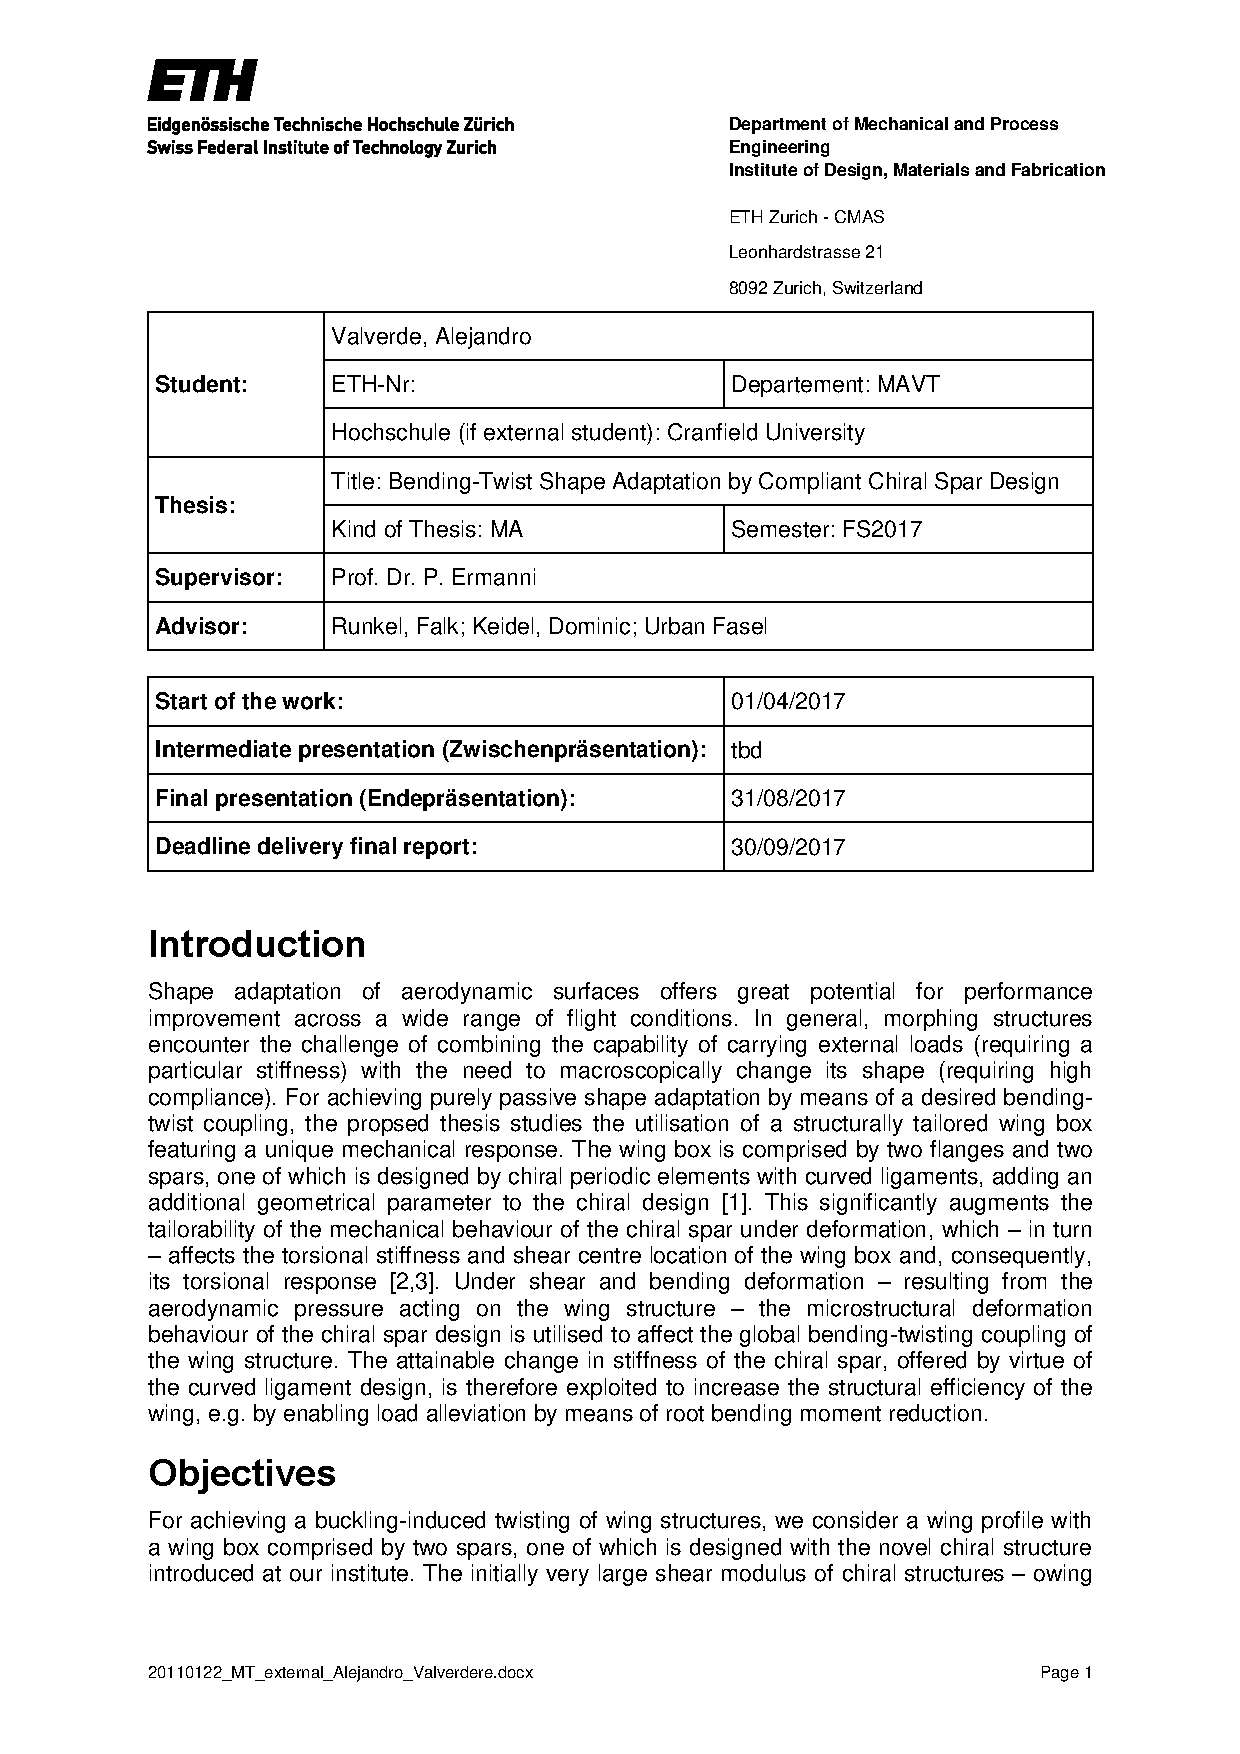
\includepdf[pages={-}]{pictures/Task_Assignement.pdf}

	%Declaration of originality
	\newpage
	\addcontentsline{toc}{section}{\protect\numberline{}{Declaration of Originality}}
	\markright{Declaration of Originality}
	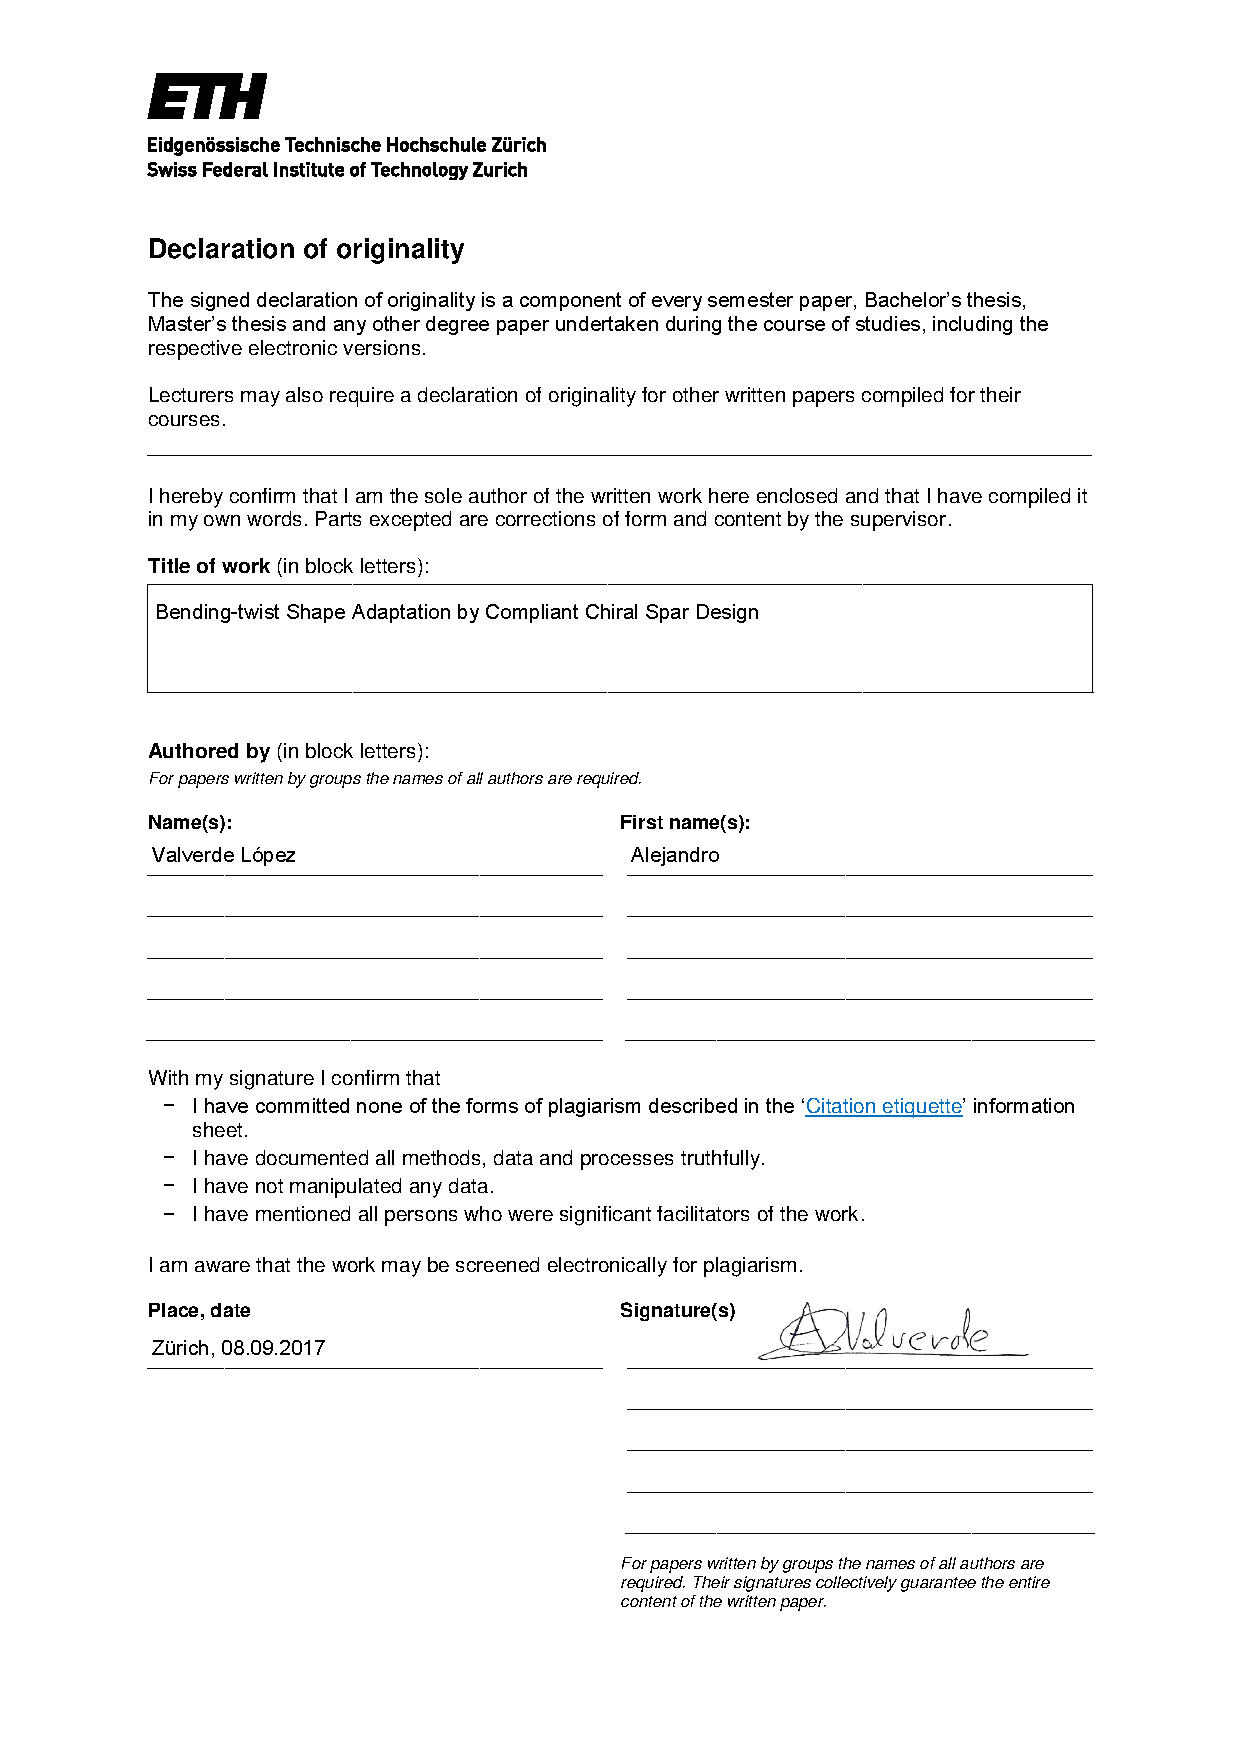
\includepdf[pages={-}]{pictures/Declaration_of_Originality.pdf}
	%ETH option
	}{\ifthenelse{\equal{\typeThesis}{CRANFIELD}}{
	%CRANFIELD option
	%CRANFILED option
	}}

%%%%%%%%% Lists %%%%%%%%%%%%%%%%%%
% Contents
\newpage
\thispagestyle{plain}
\tableofcontents
\thispagestyle{plain} %Now the plain style will be applied to all the pages of this section


% List of Figures
\newpage
\thispagestyle{plain}
\listoffigures
\thispagestyle{plain} %Now the plain style will be applied to all the pages of this section
\addcontentsline{toc}{section}{\protect\numberline{}{List of figures}}

% List of Tables
\newpage
\thispagestyle{plain}
\listoftables
\thispagestyle{plain} %Now the plain style will be applied to all the pages of this section
\addcontentsline{toc}{section}{\protect\numberline{}{List of tables}}


% Abbreviations
\newpage
\thispagestyle{plain}
%0.Nomenclature
% [a] -> For roman letters
% [b] -> For greek letters
% [c] -> For abbreviations
% [d] -> For configurations
% Example: \nomenclature[a]{$X$}{Force along x axis\nomunit{N}}
%           \nomenclature[b]{$\alpha$}{angle of attack of the aircraft \nomunit{deg}}
\nomenclature[a]{$A$}{Cross sectional area \nomunit{mm$^2$}} %Import nomenclature, no text is written
\printnomenclature[0.75in]
\addcontentsline{toc}{section}{\protect\numberline{}{List of symbols}}
\addtocontents{toc}{\vspace{.5\baselineskip}} %Small gap in the table of contents to separate entries
\thispagestyle{plain} %Now the plain style will be applied to all the pages of this section
% \section*{Abbreviation}
\label{cha:Nomenclature}
\begin{table*}[h]
\begin{tabular}{ll}
	Abbreviation & Explanations \\
\end{tabular}
\end{table*}
\newpage
\section*{List of symbols}
\renewcommand{\nomname}{}
\printnomenclature
%%Last but not least

\clearpage
\pagestyle{fancy}
\pagenumbering{arabic}

% Main part
\section{Introduction}
\label{cha:introduction}
Das ist ein Beispieltext der dauernd wiederholt wird um die Seite zu überprüfen.
Das ist ein Beispieltext der dauernd wiederholt wird um die Seite zu überprüfen.  Das ist ein Beispieltext der dauernd wiederholt wird um die Seite zu überprüfen. \footnote{test} Das ist ein Beispieltext der dauernd wiederholt wird um die Seite zu überprüfen. Das ist ein Beispieltext der dauernd wiederholt wird um die Seite zu überprüfen. \footnote{test} Das ist ein Beispieltext der dauernd wiederholt wird um die Seite zu überprüfen. Das ist ein Beispieltext der dauernd wiederholt wird um die Seite zu überprüfen. Das ist ein Beispieltext der dauernd wiederholt wird um die Seite zu überprüfen. Das ist ein Beispieltext der dauernd wiederholt wird um die Seite zu überprüfen. Das ist ein Beispieltext der dauernd wiederholt wird um die Seite zu überprüfen. Das ist ein Beispieltext der dauernd wiederholt wird um die Seite zu überprüfen. Das ist ein Beispieltext der dauernd wiederholt wird um die Seite zu überprüfen. Das ist ein Beispieltext der dauernd wiederholt wird um die Seite zu überprüfen. 
\begin{figure}[h]
	\centering
	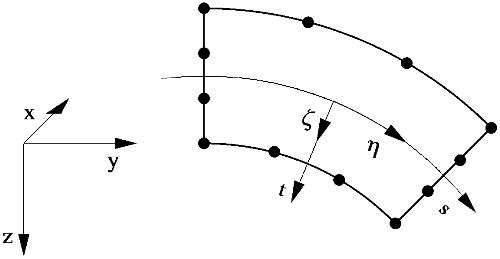
\includegraphics[width=0.6\textwidth]{pictures/ICCM20_Figure2.jpg}
	\caption{Definition of the coordinate system}
	\label{fig:arni}
\end{figure}
Das ist ein Beispieltext der dauernd wiederholt wird um die Seite zu überprüfen. Das ist ein Beispieltext der dauernd wiederholt wird um die Seite zu überprüfen. Das ist ein Beispieltext der dauernd wiederholt wird um die Seite zu überprüfen. Das ist ein Beispieltext der dauernd wiederholt wird um die Seite zu überprüfen. Das ist ein Beispieltext der dauernd wiederholt wird um die Seite zu überprüfen. Das ist ein Beispieltext der dauernd wiederholt wird um die Seite zu überprüfen. Das ist ein Beispieltext der dauernd wiederholt wird um die Seite zu überprüfen. Das ist ein Beispieltext der dauernd wiederholt wird um die Seite zu überprüfen. Das ist ein Beispieltext der dauernd wiederholt wird um die Seite zu überprüfen. Das ist ein Beispieltext der dauernd wiederholt wird um die Seite zu überprüfen. Das ist ein Beispieltext der dauernd wiederholt wird um die Seite zu überprüfen. Das ist ein Beispieltext der dauernd wiederholt wird um die Seite zu überprüfen. Das ist ein Beispieltext der dauernd wiederholt wird um die Seite zu überprüfen. Das ist ein Beispieltext der dauernd wiederholt wird um die Seite zu überprüfen. Das ist ein Beispieltext der dauernd wiederholt wird um die Seite zu überprüfen. Das ist ein Beispieltext der dauernd wiederholt wird um die Seite zu überprüfen. Das ist ein Beispieltext der dauernd wiederholt wird um die Seite zu überprüfen. Das ist ein Beispieltext der dauernd wiederholt wird um die Seite zu überprüfen. Das ist ein Beispieltext der dauernd wiederholt wird um die Seite zu überprüfen. Das ist ein Beispieltext der dauernd wiederholt wird um die Seite zu überprüfen. Das ist ein Beispieltext der dauernd wiederholt wird um die Seite zu überprüfen. Das ist ein Beispieltext der dauernd wiederholt wird um die Seite zu überprüfen. Das ist ein Beispieltext der dauernd wiederholt wird um die Seite zu überprüfen. Das ist ein Beispieltext der dauernd wiederholt wird um die Seite zu überprüfen. Das ist ein Beispieltext der dauernd wiederholt wird um die Seite zu überprüfen. Das ist ein Beispieltext der dauernd wiederholt wird um die Seite zu überprüfen. Das ist ein Beispieltext der dauernd wiederholt wird um die Seite zu überprüfen. Das ist ein Beispieltext der dauernd wiederholt wird um die Seite zu überprüfen. Das ist ein Beispieltext der dauernd wiederholt wird um die Seite zu überprüfen. Das ist ein Beispieltext der dauernd wiederholt wird um die Seite zu überprüfen. Das ist ein Beispieltext der dauernd wiederholt wird um die Seite zu überprüfen. Das ist ein Beispieltext der dauernd wiederholt wird um die Seite zu überprüfen. Das ist ein Beispieltext der dauernd wiederholt wird um die Seite zu überprüfen. Das ist ein Beispieltext der dauernd wiederholt wird um die Seite zu überprüfen. Das ist ein Beispieltext der dauernd wiederholt wird um die Seite zu überprüfen. Das ist ein Beispieltext der dauernd wiederholt wird um die Seite zu überprüfen. Das ist ein Beispieltext der dauernd wiederholt wird um die Seite zu b
\ClearDoublePageOrNot{\controlClearPage}
\chapter{State-of-the-art} \label{chap:State_of_the_art}

This chapter presents a review of the current technologies related to the topic of this work will be done. Different morphing wing technologies will be introduced. Secondly, a particular focus on the state-of-the-art of technology exploit in the current project will be presented.

\section{Morphing aircraft} \label{sec:Morphing_state}

  %A little bit of Wright Brothers
  Their concept of aircraft did not provide importance to built-in stability but absolute control of the aircraft by the pilot. For this reason, they deliberatively designed their first aircraft with anhedral wing that make it dynamically unstable to perturbations in sideslip but more maneuverable in the lateral direction. In order to achieve roll control, they decided to incorporate a mechanism that would allow the wings to twist by pulling from cables, as it can be seen in Figure \ref{fig:Wright}. This was the first ever use of morphing of an aerodynamic surface for aircraft control.

  \begin{figure}[!htpb]
    \centering
    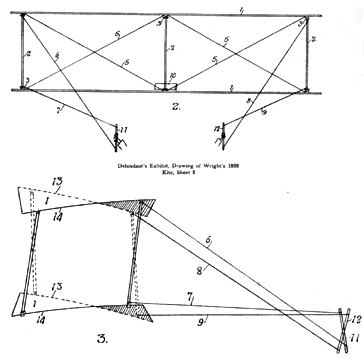
\includegraphics[width=0.5 \textwidth]{state-of-the-art/WrightBrothers1899Kite}
    \caption[Wright Brothers 1899 kite]{Wright Brothers 1899 kite: front and side views, with control sticks. Wing-warping is shown in lower view. \cite{Wright}}\label{fig:Wright}
  \end{figure}

  %Why now?
  New interest has raised in the recent years in aircraft morphing, mainly due to the appearance of new smart materials that allow more efficient mechanical design that do not necessarily incur in weight increments \cite{Lloyd2007}. Another reason that is pushing forward new aircraft morphing technologies is that missions today are in need of higher aircraft versatility to decrease operational costs in the commercial aviation field and aim to smaller and more distributed targets in the military field. For example, Airbus has recently patented a design of a downwardly foldable wing tip device applicable for a large passenger aircraft \cite{Boye2015}.

  %Different morphing projects - \cite{Barbarino}
  A general classification of different wing morphing concepts can be seen in Figure \ref{fig:morphingTypes}: planform modification through variation of sweep angle, span or chord; out-of-plane alteration involving twist, dihedral angle and spanwise bending, and airfoil adjustment achieved by modifications of the airfoil chamber and/or thickness. Under this classification, the morphing technology that is the focus of the work presented in this thesis is located under the out-of-plane branch and twist modification.

  \begin{figure}[!htpb]
    \centering
    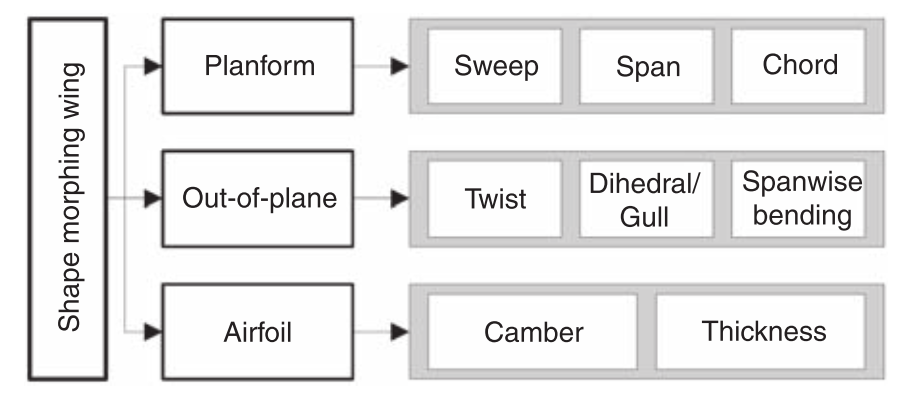
\includegraphics[width=0.8 \textwidth]{state-of-the-art/morphingTypes}
    \caption[Shape morphing wing classification]{Shape morphing wing classification. \cite{Barbarino2011}}\label{fig:morphingTypes}
  \end{figure}

  %NASA morphing proyect
  In the field of wing morphing through active aeroelastic concepts, the pioneer program of the Active Flexible Wing (AFW) was developed by Rockwell International in the 1980s \cite{Rockwell}. Under this program, a design of an aircraft where the wing aeroelastic twist was used to produce the required roll moments for control was generated. This enabled the aircraft to operate at dynamic pressures beyond those where convectional ailerons suffer from the appearance of reversal aeroelastic instabilities. Later, NASA continued with the AFW concept within their Active Aeroelastic Wing (AAW) project which used a modified F-18 fighter named X-53 to perform flight test and assess the viability of the proposed concept. A picture showing this aircraft can be seen in Figure \ref{fig:x-53}. The X-53 had its wings modified to reduce the torsional stiffness and had additional actuators added to operate the outboard leading-edge flaps separately from the inboard leading-edge surfaces \cite{NASA}. Rolling moment was obtained by aeroelastic twist of the wing using trailing-edge control surfaces and leading-edge flaps.

  \begin{figure}[!htpb]
    \centering
    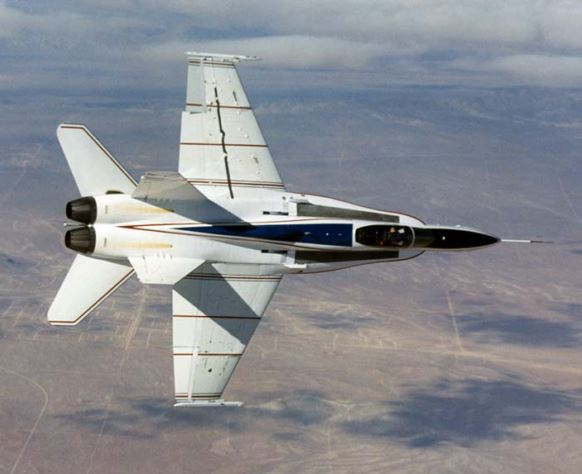
\includegraphics[width=0.6 \textwidth]{state-of-the-art/x-53}
    \caption[The X-53 performing a 360$^{\circ}$ roll to prove AAW technology]{The X-53 performing a 360$^{\circ}$ roll to prove AAW technology. \cite{NASA}}\label{fig:x-53}
  \end{figure}

  %Here, many more references can be included by looking at Barbarino2011, maybe later... \section{Wing twist morphing}
  Following that initial attempts , many additional research literature can be found for other approaches. Many of those, consisted in modifying the wing properties by active means, i.e.: incorporating actuators that introduce energy into the system. Among the vast available literature in this field, it is worth mentioning the advances made in \cite{Chen2000} by the development of a variable stiffness spar (VSS) concept to control the torsional stiffness as a function of the Mach number and the altitude. Also, in the investigation presented by \cite{Amprikidis2005}, the adaptive torsional stiffness for a vertical tail was achieved by a variable attachment point position. The work presented by \cite{Stanford2007} showed how roll control of a small aircraft could be achieved by actively twisting its flexible wing. The technology of the shape memory alloys (SMA) has been also exploit in the field of active wing twist morphing, as seen in \cite{Sanders2001} and \cite{Elzey2003}.

  However, wing twist morphing designs may also benefit from geometrically flexible structures if the aeroelastic energy from the airstream can be used to activate the shape changing mechanics. Such an approach may lead to passive morphings strategies that are always preferred since no additional energy is necessary to be introduced into the system and the usual weight penalties of morphing may be avoided if no additional actuators are needed. 

  In \cite{Arrieta2014}, a passively triggered system to reduce the lift increment that follows a gust encounter using multi-stable elements embedded into the airfoil is presented. Other examples of wing twist morphing by passive means are those presented in \cite{Bornengo2005}, \cite{Spadoni2007a} and \cite{Spadoni2007b}. In particular, the technology proposed in these works exploits the capabilities of the chiral structures that feature a negative Poisson's ratio for in-plane strains. A network of these chiral structure is embedded in the rib of the airfoil constituting the deformable part. These chiral structures will be extensively discussed in the next section.

  %%% Bending-Twist shape adaptation by compliant structural designs
  %Mention-> Falk's work, compare with the actual design proposal (chiral structure): Compliant Chiral Spar Design, 
  %
  % by designing structural components in which instability occurs in a deliberate way. For that purpose, a structural tailoring procedure providing a particular material anisotropy by varying fibre orientation and thickness of the component is introduced.
  % carbon fibre reinforced plastic (CFRP)
  %
  Also in the field of passive approaches to achieve wing twist morphing, W. Raither proposed in \cite{Raither2013a} a novel concept of adaptive aeroelastic tailoring by means of the wing-box torsional stiffness modification. In order to achieve this, the shear stiffness $G t$ of one of the webs that conform the wing-box beam is modified. This induces the section's shear centre shifting, which provides an additional torsional deformation for a constant load. This concept is later explained in Section \ref{sec:concept_Model} as the same working principle is used for the technology presented in this work.

  Implementation of the proposed principle requires a material with controllable in-plane shear modulus. A possible solution is proposed in \cite{Bergamini2006} and consisted in the use of electro-bonded laminates that vary its bending stiffness by means of electrostatic forces applied different at points of the structure. Another approach is presented in \cite{Raither2012}, and exploits the time-variable lamination in laminate composite shells provided by the temperature dependence of the elastic modulus of polymers in proximity of their glass transition. Therefore, the proposed concept consists on a semi-passive approach since some energy needs to be spent for the activation of the adaptive interfaces. In \cite{Raither2013} the demonstrator shown in Figure \ref{fig:raither-demonstrator} was built to show the viability of this last approach.

  \begin{figure}[!htpb]
    \centering
    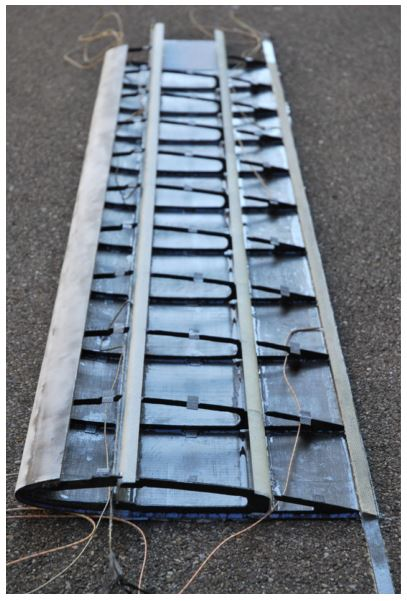
\includegraphics[width=0.6 \textwidth]{state-of-the-art/raither-demonstrator}
    \caption[Inner structure of the experimental wing build to test the concept of adaptive wing-box]{Inner structure of the experimental wing build to test the concept of adaptive wing-box. \cite{Raither2013}}\label{fig:raither-demonstrator}
  \end{figure}

  Finally, in \cite{Runkel2016} the variation of in-plane shear modulus is proposed that can be achieved by inducing elastic instabilities on one of the webs of the wing-box. The component is manufactured with a particular material anisotropy utilizing unidirectional CFRP. The appearance of plate buckling at the root on the specially designed web, as shown in Figure \ref{fig:plate-buckling}, induces the shear centre location shifting and the torsional stiffness of the structure, thus leading to a purely passive bending-twist coupling. In \cite{Andreas2015}, the mechanical response was investigated using FE simulations and experimental testing on a manufactured demonstrator of the concept.

  \begin{figure}[!htpb]
    \centering
    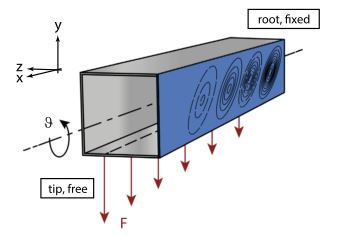
\includegraphics[width=0.7 \textwidth]{state-of-the-art/plate-buckling}
    \caption[Plate bucking on one of the webs of the wing-box beam]{Plate bucking on one of the webs of the wing-box beam. The drawing shows a qualitative view of the buckling field. \cite{Runkel2016}}\label{fig:plate-buckling}
  \end{figure}

\clearpage
\section{Compliant chiral structure} \label{sec:chiral_state}
  % \citeauthor{Lakes1991}
  % \citeauthor{Bornengo2005}
  % \citeauthor{Prall1997}

  As mentioned in the introduction, it is the interest of this work to use structures that have recently been of interest due to its capabilities as materials with negative Poisson's ratio. Such materials expand laterally when stretched and contract laterally when compressed. In \cite{Lakes1991}, R. Lakes proposed that negative Poisson's ratios can result from a hexagonal microstructure of rotable nodes and bendable ligaments such as the one shown in Figure \ref{fig:chiral}. Such structures are known as non-centrosymmetric, hemitropic, or chiral; they are distinguishable from their mirror image; that is, they cannot be superposed onto them and they are not isotropic.

  \begin{figure}[!htpb]
    \centering
    
\includegraphics[width=0.6 \textwidth]{state-of-the-art/chiral}
    \caption[Chiral structure of rotable nodes and bendable ligaments]{Chiral (noncentrosymmetric) hexagonal microstructure of rotable nodes and bendable ligaments. Poisson's ratio is negative. \cite{Lakes1991}}\label{fig:chiral}
  \end{figure}

  In \cite{Prall1997}, experimental results showed that the a honeycomb chiral structure exhibited a Poisson's ratio of -1 for deformations in-plane. Indeed, this behavior was maintained over a significant range of strain, as shown in Figure \ref{fig:experimentalPoisson}, and therefore verifying that Poisson's ratio is independent upon the strain, in agreement with theory. 
  \begin{figure}[!htpb]
    \centering
    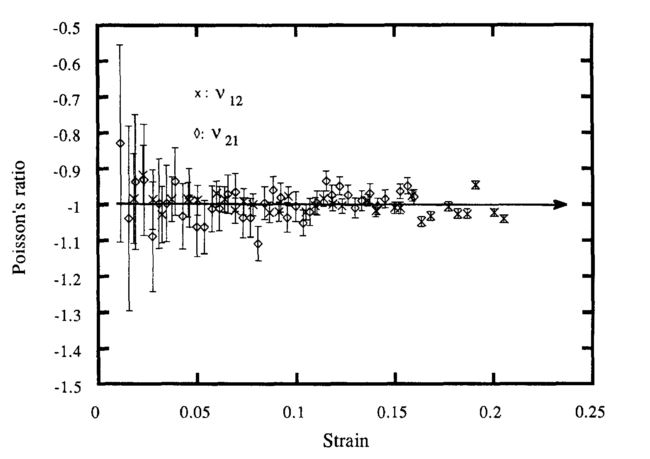
\includegraphics[width=0.8 \textwidth]{state-of-the-art/experimentalPoisson}
    \caption[Experimental Poisson's ratio $v$ as a function of axial compressive strain on a chiral honeycomb]{Experimental Poisson's ratio $\nu$ as a function of axial compressive strain on a chiral honeycomb. The error bars represent inaccuracies due to the measurement resolution. \cite{Prall1997}}\label{fig:experimentalPoisson}
  \end{figure}

  In \cite{Bettini2010} the properties of a chiral honeycomb are investigated, a manufacturing process using composite materials is proposed and the increase in the performance of using such materials is shown. Also, the experiments carried out allowed to characterize the possible failure modes of this structures and the nonlinear response when large displacements occur.

  Until that moment, most of the work was concentrated in studying the in-plane behavior of the chiral structures. Then, in \cite{Spadoni2005} the flatwise compression behavior of the chiral structures is investigated through FE modeling and simply analytical relations. This is the first consideration of buckling in a chiral structure in some way, in this case it was the out-of-plane buckling behavior based on the similar works presented in \cite{Zhang1992} and \cite{Gibson1999} for honeycomb structures. This research was extended by experimental studies in \cite{Scarpa2007} and an anelastic characterization of the buckling phenomena is presented in \cite{Miller2010}. The buckling response of chiral honeycombs under a general macroscopic in-plane stress state was more recently investigated from a theoretical point of view in \cite{Haghpanah2014}. 

  %Buckling - Reference to work done by Gilles
  Within the research undertaken at the Laboratory for Composite Materials and Adaptive Structures (CMAS) of the ETH Z\"urich in the field of variable stiffness structures, a novel chiral topology has recently been proposed. The chiral unit cell is modified by introducing transverse curvature into the ligaments, as shown in Figure \ref{fig:ramstein-curved}. Such design increases the bending stiffness of the ligament and thus of the entire periodic structure. Each ligament posses double eccentricity which changes orientation at the centerline of it, in compliance with a equivalent connection with the cylinders located at the extremes. In \cite{Ramstein2016} preliminary investigations of such structures were experimentally conducted on a conceptual level for a basic triangular chiral structure, as shown in Figure\ref{fig:basic-triangular-test}.

  \begin{figure}[!htpb]
    \centering
    \subfigure[Flat ligaments.]{\label{fig:ramstein-flat}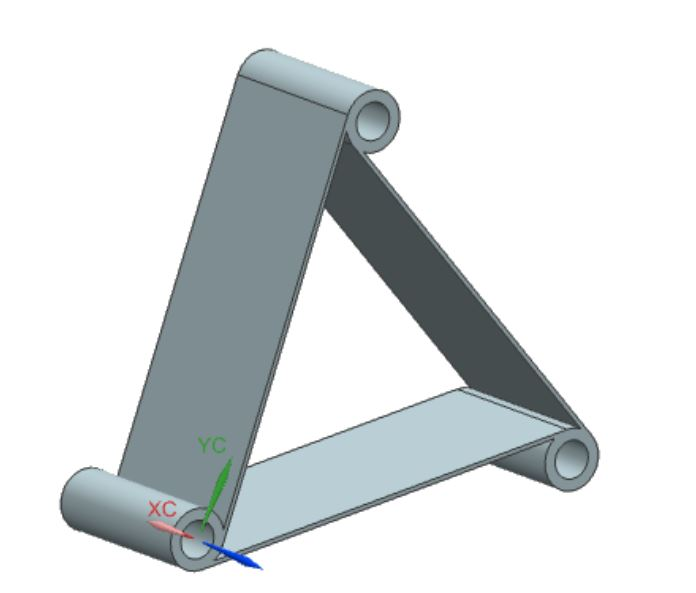
\includegraphics[width=0.4\textwidth]{state-of-the-art/flat-ligaments}} \qquad
    \subfigure[Curved ligaments.]{\label{fig:ramstein-curved}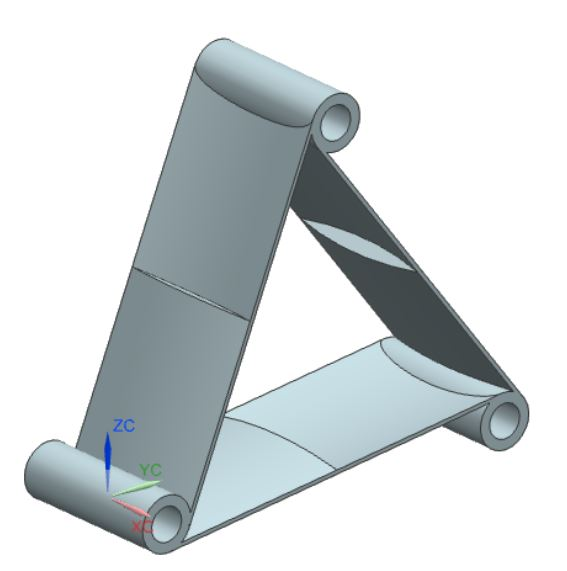
\includegraphics[width=0.35\textwidth]{state-of-the-art/curved-ligaments}}
    % \begin{subfigure}{0.5\textwidth}
    %   \centering
    %   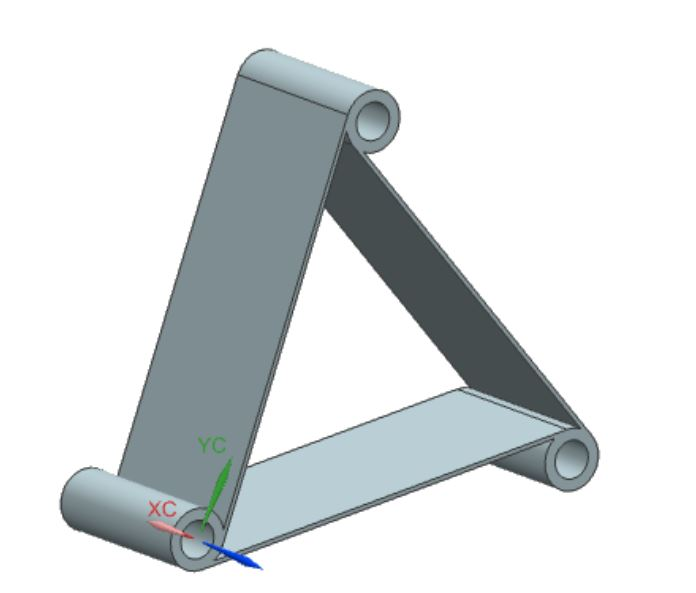
\includegraphics[width=0.4\linewidth]{state-of-the-art/flat-ligaments}
    %   \caption{Flat ligaments.}
    %   \label{fig:ramstein-flat}
    % \end{subfigure}%
    % \begin{subfigure}{0.5\textwidth}
    %   \centering
    %   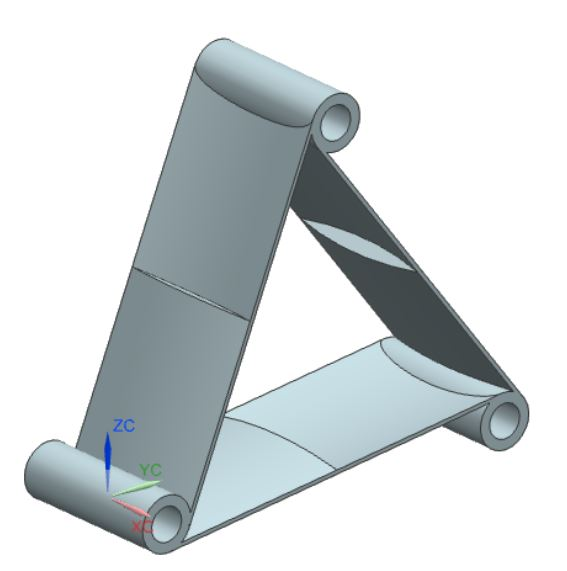
\includegraphics[width=0.4\linewidth]{state-of-the-art/curved-ligaments}
    %   \caption{Curved ligaments.}
    %   \label{fig:ramstein-curved}
    % \end{subfigure}
    \caption[Chiral cell elements showing different ligaments curvatures]{Chiral cell elements showing different ligaments curvatures. \cite{Ramstein2016}}
    \label{fig:ramstein}
  \end{figure}

  \begin{figure}[!htpb]
    \centering
    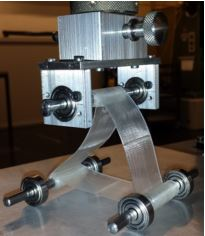
\includegraphics[width=0.5 \textwidth]{state-of-the-art/basic-triangular-test}
    \caption[Compression load test on a basic triangular chiral structure]{Compression load test on a basic triangular chiral structure. \cite{Ramstein2016}}\label{fig:basic-triangular-test}
  \end{figure}

  This new design of the ligaments will provide additional tailorability over the buckling phenomena occurring on the lattice ligaments. This configuration is the one chosen for the chiral structure that is used in the concept presented in this work.

  Different approaches has been followed to exploit the particular characteristics of chiral structures under in-plane strain, on aerodynamic elements such as airfoils. In \cite{Bornengo2005} a truss-core configuration such as the one shown in Figure \ref{fig:truss-core-airfoil}(a) with chiral topology was utilized to design an airfoil for automotive competitions. The concept exploits the elastic deformation of the chiral lattice to modify the airfoil mean chamber line and thus modifying the pressure distribution as required for the current desired performance of the car. In \cite{Spadoni2007a}, a similar configuration was investigated by weakly coupled structural and CFD models, and the local and global deformations were characterized by consideration of the macroscopic chiral configuration. A prototype of the proposed design, as shown in Figure \ref{fig:truss-core-prototype}, was manufactured and tested in \cite{Spadoni2007b}. Results showed a remarkable tailoring of the chamber morphing performance by means of a limited number of parameters which define the core geometry. The dynamic properties of such chiral truss-core assemblies were investigated in \cite{Spadoni2006}.

  \begin{figure}[!htpb]
    \centering
    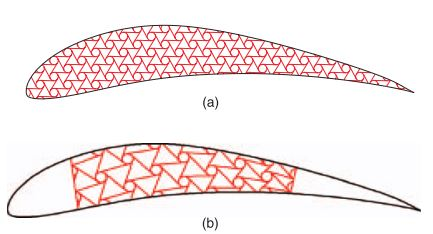
\includegraphics[width=0.7 \textwidth]{state-of-the-art/truss-core-airfoils}
    \caption[Investigated configurations for the truss-core of chiral topology]{Investigated configurations for the truss-core of chiral topology. \cite{Spadoni2007a}}\label{fig:truss-core-airfoil}
  \end{figure}

  \begin{figure}[!htpb]
    \centering
    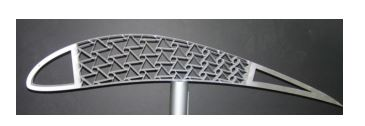
\includegraphics[width=0.8 \textwidth]{state-of-the-art/truss-core-prototype}
    \caption[Manufactured prototype of a truss-core airfoil with chiral topology]{Manufactured prototype of a truss-core airfoil with chiral topology. They were manufacture in aluminum, using water-jet cutting techniques. \cite{Spadoni2007b}}\label{fig:truss-core-prototype}
  \end{figure}

  Recently, A. Airoldi developed the ``chiral sail'' concept in \cite{Airoldi2012} which exploits the chiral topology of a chiral network embedded into the airfoil rib. The pressure difference between the upper and lower parts of the airfoil promotes the chamber variation as shown in Figure \ref{fig:chiral-sail} and amplifying the lift when the angle of attack increases. This concept was implemented and validated by testing a demonstrator in \cite{Airoldi2015a}. The experimental side of this work showed the difficulties of manufacturing such complex structures.

  \begin{figure}[!htpb]
    \centering
    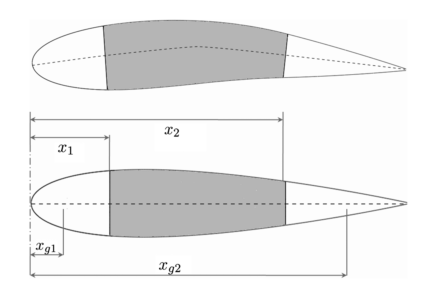
\includegraphics[width=0.8 \textwidth]{state-of-the-art/chiral-sail}
    \caption[Chiral sail concept]{Chiral sail concept. The rib of the airfoil is constituted of a network of chiral unit cells. \cite{Airoldi2012}}\label{fig:chiral-sail}
  \end{figure}  

\clearpage
\section{Rationale for the thesis} \label{sec:rationale_state}

  This thesis is part of the current research that it is been carried out at CMAS in seek of wing twist morphing achieved through variable stiffness wing-box structures that acquire this property undergoing elastic instabilities. 

  As shown in the topic review presented in \cite{Hu2015} and \cite{Reis2015}, the use of buckling-induced technologies is a promising technique to achieve the desired behavior in recent developments of smart structures. Traditionally, elastic instabilities were avoided in the structural designs due to the significant loss of load-carrying capacity and the large deformations occurring as a consequence of such an event. However, in the scope of the so called motion-related applications of buckling-induced technologies, the capability of small perturbations to generate sudden snapping behavior in elastic elements enables the structure to dynamically change its configuration, being this beneficial for applications such the one considered in the present work. Also, the possibility of minimizing the actuation force required during shape recovery due to the elastic state of the structure becomes interesting.

  In parallel, when it comes to the bending-twist shape adaptation by compliant structural designs, some of the solutions already introduced in this chapter are able to modify the wing-box torsional stiffness for a pre-defined shape variation or are optimized for a given actuation lay-out, whereas the adoption of a structural concept such as a chiral lattice offers a wide range of possibilities in terms of tailoring. In particular, the chiral structures that posses curved ligaments are the design option for the concept proposed in this work. This novel characteristic is expected to provide additional control over the buckling appearance and evolution. This design of chiral structure was already manufactured and tested in another project completed at CMAS \cite{Vincenz2017}.

  Thereby, for the approach presented in this work, the working principle introduced by \cite{Raither2013a} is combined with the buckling capabilities of the chiral structures exposed in Section \ref{sec:chiral_state} to conform the proposed principle. 

  In the scope of this thesis, a full model of the whole wing-box with the compliant variable-stiffness spar is studied. It is the intention to look at the buckling characteristics of the lattice of chiral structures that conforms the spar and the response in twist of the whole assembly. It is expected to see buckling occurring on several ligaments at the same time at of those located close to the root of the wing-box. Also, it is envisioned that the buckling phenomena activates a sudden change in the twist of the wing-box. Also, the modification of internal parameters of the chiral structure is expected to show promising tailorability capabilities on the force-displacement curve.

  It is expected that the proposed technology will be suitable for environments where a rapid shape adaptation is required. Such applications may include to increase the critical speed for load alleviation purposes.

  In order to achieve verification of the previous premises, a numerical and analytical model model will be built of the whole wing-box assembly. The evolution of the buckling phenomena for in the structure will be characterized and the effect of the different design parameters on the structure pre-buckling and post-buckling response will be assessed. The aim is to provided a suitable computational environment to achieve in-deep understanding of the proposed working principle and assist the manufacture of a future demonstrator.

\ClearDoublePageOrNot{\controlClearPage}
\chapter{Wing-box model} \label{chap:Model}

\section{Introduction} \label{sec:intro_Model}

  In the present chapter the model used for the wing-box design is presented. On first place, the working principle of the technology that it is the topic of this work is presented.

  Next, the two different models developed to provide fully understanding of the structure response are presented. Firstly, a simple analytical model is presented to provide fast insight of the role of each of the parameters that characterize the ideal beam configuration of a beam with a web featuring variable stiffness properties. Important relevance is given to the section's shear centre $y_{\mathrm{SC}}$ shifting as this variable determinate the magnitude of the resulting torsional moment action on the beam as a result of a load acting on the beam's transversal plane.

  Secondly, the computational model is introduced. The different constituting elements are explained together with the boundary conditions, loads and mesh that are used in the simulations 

  Finally, the program used to carry out automatic parametric studies is presented, together with its methodology.

\section{Concept} \label{sec:concept_Model}
  %
  % Explanation of the concept
  % -> Bending-twist coupling
  % -> Shiftable shear centre location
  % -> A web with variable-stiffness capability
  %
  % Figure: Fig. 1 Raither ?, Geometry and system of coordinates.
  % Figure: Fig. 2 Raither ?, Schematic of the working principle.
  %
  %Chiral structure
  %View Airoldi (2012)
  %
  % -> Buckling phenomena
  % Figure: Schematic representation buckling phenomena

  As it was already introduced in last chapter, the proposed technology to achieve twist morphing through a variable torsional stiffness wing-box is based on the working principle presented in \cite{Raither2013a} and exploits the buckling characteristics of a lattice of chiral ligaments as a way of varying the stiffness on the adaptive spar of the wing-box.

  The basic working principle consisted on employing profile beams in which the shear centre is shifted as a result of the variable-stiffness capability of one of the webs. An schematic view of the working principle is shown in Figure \ref{fig:adaptive-beam-concept} where an adaptive beam is displayed. In Figure \ref{fig:adaptive-beam-concept}(a), the four webs that constitute the rectangular profile of the beam have the same shear stiffness $G_2 t_2 = G_1 t_1$. The double symmetry characteristic of such a configuration indicates that the shear centre is located at the point where the two symmetry axes intersect. For this case, under a load applied on the shear centre, the beam experiences bending deformation with null twist. On the other hand, when considering the situation shown in Figure \ref{fig:adaptive-beam-concept}(b) where $G_1 t_1 > G_2 t_2$, the reduced shear stiffness of the adaptive web produces that shear centre moves along the $y$ direction and towards positive values of $y$. In this case, if the load is maintained in the same application point as before, the beam experiences bending deformation and negative twist. Correspondingly, for the case shown in Figure \ref{fig:adaptive-beam-concept}(b) where $G_2 t_2 > G_1 t_1$, the shifting of the shear centre is towards negative values of $y$ and the beam experiences a positive twisting under the prescribed load.

  \begin{figure}[!htpb]
    \centering
    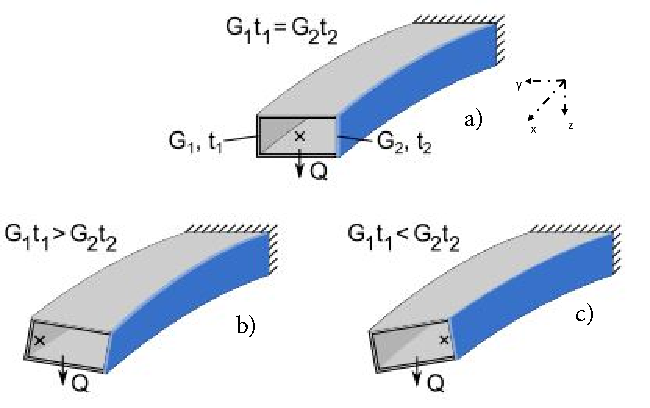
\includegraphics[width=0.7 \textwidth]{state-of-the-art/adaptive-beam-concept}
    \caption[Working principle for the adaptive beam]{Working principle for the adaptive beam. \cite{Raither2013}}\label{fig:adaptive-beam-concept}
  \end{figure}

  The bending-twist coupling of the beam can therefore be controlled by the variable-stiffness web. The properties of the web can be modified by either adjusting the shear modulus $G_2$ or the thickness $t_2$ of the web. 

  In the technology presented in this work, the adaptive web is constituted of a lattice of chiral structures. On these elements, elastic buckling is intentionally induced and the resulting consequence is the reduction of the overall shear modulus $G_2$ effectively introducing an effective shear modulus $G_{2,\mathrm{eff}} < G_1$. An example of the chiral structure undergoing buckling instabilities can be seen in Figure \ref{fig:bucklingChiral}.

  \begin{figure}[!htpb]
    \centering
    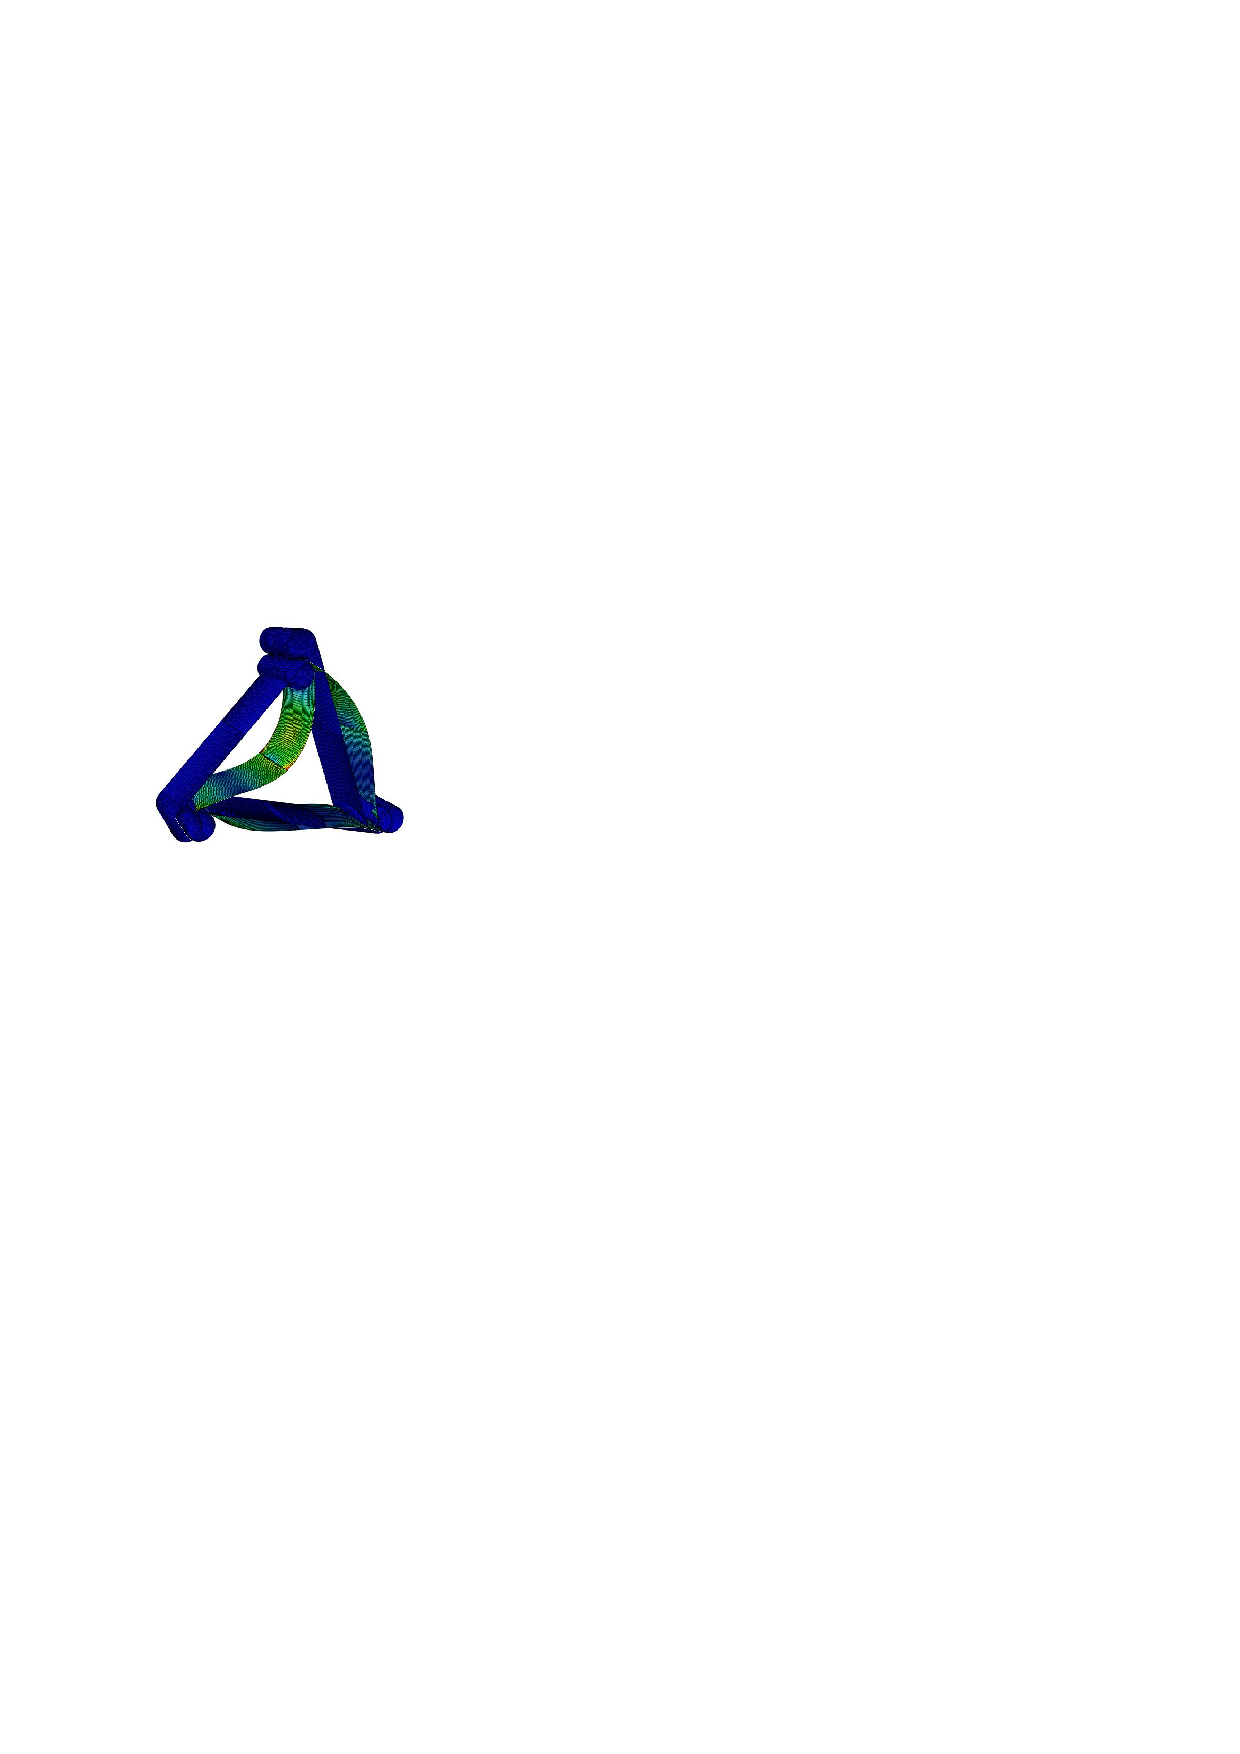
\includegraphics[width=0.5 \textwidth]{state-of-the-art/bucklingChiral}
    \caption[Chiral unit cell undergoing buckling instabilities]{Chiral unit cell undergoing buckling instabilities. \cite{Ramstein2016}}\label{fig:bucklingChiral}
  \end{figure}

  % wHAT'S THE ROLE OF ALL THIS IF BUCKLING IS NOW USED????
  % As shown in Section \ref{sec:chiral_state}, the negative Poisson’s ratio behavior leads to unique deformation patterns, and corresponds to a very high in-plane shear modulus $G$, as shown in Equation \ref{eq:shearModulus} for values of Poisson's ratio $\nu \to -1$:
  % %
  % \begin{equation}\label{eq:shearModulus}
  %   G = \frac{E}{2 (1 - \nu)},
  % \end{equation}
  % %
  % where $E$ is the Young's modulus. 

\section{Analytical model} \label{sec::analytical_Model}
  %
  %% Analytical apprach description
  % An analytical model of the Wing Box will be build.
  % Shear centre calculation
  % The twist of the beam will be calculated
  %
  %Figure of analytical model

  The analytical model of the wing-box is presented in the present section. An schematic view of the section of the beam can be seen in Figure \ref{fig:analyticalBox}. The main dimensions for the section are given by the height $H$ and the width $B$. Such a structure if characterized by having three elements with identical thickness $t_1$, shear modulus $G_1$ and Young's modulus $E_1$. For the element on the right, the adaptive web, the same parameters are $t_2$, $G_2$ and $E_2$, respectively. 

  \begin{figure}[!htpb]
    \centering
    
\includegraphics[width=0.7 \textwidth]{model/analyticalBox2}
    \caption[Schematic view of the beam closed section]{Schematic view of the beam closed section. The dimensions are given by the width $B$ and the height $H$. For the upper, lower and left elements, the wall thickness, shear modulus and the Young's modulus are given by $t_1$, $G_1$ and $E_1$, respectively. For the right element, the same parameters are given by $t_2$, $G_2$ and $E_2$.}\label{fig:analyticalBox}
  \end{figure}

  As explained in Section \ref{sec:concept_Model}, the shear stiffness $G t$ of the adaptive web can be modified by varying either thickness $t$ or shear modulus $G$. For the remaining, it is assumed that $t_1 = t_2 = t$ and therefore the thickness $t$ will not be considered as a modifiable parameter on the adaptive web.

  Now the bending-twisting coupling of the structure is investigated using well-know equation to describe the elastic behaviour of thin-wall beam elements. Based on the analytical approach to the problem of a beam bending-twisting coupling followed in \cite{Raither2013a}, it is known that warping can be neglected for a configuration like the one presented in this section.

  The bending displacement of the structure is therefore given by Equation \ref{eq:wb} which a solution of the well-know Bernoulli-Euler equation for a beam:

  \begin{equation}\label{eq:wb}
    w_b = \frac{Q L^3}{6 \Phi_y} \left( -\frac{x^3}{L^3} + \frac{3 x^2}{L^2} \right),
  \end{equation}
  %
  where $w_b$ is the displacement along the $z$ direction and $\Phi_y$ is the flexural stiffness given by Equation \ref{eq:flexuralStiffness}:
  %
  \begin{equation}\label{eq:flexuralStiffness}
    \Phi_y = \int \int E(y,z) z^2 \mathrm{d}y \mathrm{d}z.
  \end{equation}

  %Twist
  On the other hand, the twist of a beam with closed section can be obtained from the St. Venant expression for the specific twist $\vartheta$, which is shown in Equation \ref{eq:specificTwist}:
  %
  \begin{equation}\label{eq:specificTwist}
    \vartheta = \frac{\mathrm{d} \phi}{\mathrm{d} x} = \frac{M_t}{4 A_0^2} \oint \frac{\mathrm{d} s}{Gt},
  \end{equation}
  %
  where $A_0$ represent the area enclosed by the profile's wall midline, $\phi$ is the twist of the beam and $M_t$ is the torsional moment applied. Additionally, the torsional stiffness for the closed section under study is given by the Equation \ref{eq:torStiff}:
  %
  \begin{equation}\label{eq:torStiff}
    G I_t = \frac{4 A_0^2}{\oint \frac{\mathrm{d} s}{G(s) t(s)}}.
  \end{equation}

  In order to calculate the specific twist $\vartheta$ , it is necessary to evaluate the shear centre position $y_{\mathrm{SC}}$ for a given configuration. In order to achieve this, evaluation of the shear flow distribution in the section also needs to be undertaken. To calculate the shear flow $q(s)$, the profile can be considered to be cut at one point, resulting on a opened section. The shear flow $q_{\parallel}(s)$ for this case can be calculated using Equation \ref{eq:shearFlowEquation}. The corresponding shear flow for a closed section can be obtained using the Equation \ref{eq:shearFlowDescomposition}:
  %
  \begin{equation}\label{eq:shearFlowEquation}
    q_{\parallel}(s) = - \frac{Q_z}{\Phi_y} S_{E_y}(s),
  \end{equation}
  %
  \begin{equation}\label{eq:shearFlowDescomposition}
    q_\mathrm{C}(s) = q_\parallel(s) + q_0,
  \end{equation}
  %
  where $Q_z$ is the force applied in the z direction and $S_{E_y}$ is the so called static moment or first moment of area, which is calculated through the integral shown in Equation \ref{eq:staticMoment}. Also, the variable $q_0$ represents the shear flow at the boundary that results from the torsion of the beam and can be calculated using the Equation \ref{eq:constantShearFlow}:
  %
  \begin{equation}\label{eq:staticMoment}
    S_{E_y}(s) = \int_0^s E(s) t(s) z(s) \mathrm{d}s,
  \end{equation}
  %
  \begin{equation}\label{eq:constantShearFlow}
    q_0 = \frac{Q_z}{\Phi_y} \frac{ \oint_s \frac{S_{E_y}(s)}{G(s) t(s)} \mathrm{d}s }{ \oint_s \frac{1}{G(s) t(s)} \mathrm{d}s }.
  \end{equation}

  Now, the shear centre position in the beam transversal section will be calculated for the case of open section. Given that beam mechanical properties and geometrical dimensions are symmetric around y axis, the shear centre position in the z axis will be $z_{\mathrm{SC}} = 0$. On the other hand, the shear centre position in the y axis will be given by the Equation \ref{eq:shearCentrePosition}:
  %
  \begin{equation}\label{eq:shearCentrePosition}
    y_{\mathrm{SC,open}} = \frac{1}{Q_z} \oint_s q_\mathrm{C}(s) r(s) \mathrm{d}s,
  \end{equation}
  %
  where $r$ represents the perpendicular distance to the coordinate origin.

  Now, it is necessary that equilibrium exists between the torsional moment due to the shift of the shear centre (caused during the opening of the profile) and the moment due to the torsional shear flow of the closed profile. This condition can be mathematically expressed through Equation \ref{eq:shearCentrePositionMoment}:
  %
  \begin{eqnarray}\label{eq:shearCentrePositionMoment}
  % \nonumber % Remove numbering (before each equation)
    M_\mathrm{t} &=& Q_\mathrm{z} (y_{\mathrm{SC,open}} - y_{\mathrm{SC,closed}}) \nonumber \\
    &=& 2 A_0 q_0.
  \end{eqnarray}
  %
  %where it has been considered that a positive moment $M_\mathrm{t}$ along the x direction produces a constant shear flow distribution which has negative sign given the shear flow distribution definition in the present text.

  Finally, the total shear flow $q(s)$ results from the superposition of the shear flow of the open profile $q_\mathrm{C}$ and the constant shear flow due to torsion $q_0$, as shown in the Equation \ref{eq:totalShearFlow}:
  %
  \begin{equation}\label{eq:totalShearFlow}
    q(s) = q_\mathrm{C}(s) - q_0. %before it was: q_\mathrm{C}(s) - q_\mathrm{M}
  \end{equation}

\section{Computational model} \label{sec:computationalModel}
  %
  % Description of the model
  %   Include all the parts of the model: C-box shape, inner box, chiral lattice
  %   Figure of the model
  % Parameters included
  %
  % Subsections:
  % - Sub-parts and parametrization of the model, include main dimensions and parameters. Sketch and Abaqus model screenshot
  %     - Lattice
  %     - Lattice nodes with tyre part
  %     - C-box
  %     - Ribs
  % - Attachment points modeling
  % - Parametric study method

  The computational model of the wing box was built using Abaqus CAE commercial software. It consisted on three main elements: the wing-box with C-profile, the lattice constituted of the chiral elements, a closed rib at the tip of the box and a closed rib at the root of the box. A general overview of the assembly of the different parts can be seen in Figure \ref{fig:all-assembly}.

  \begin{figure}[!htpb]
    \centering
    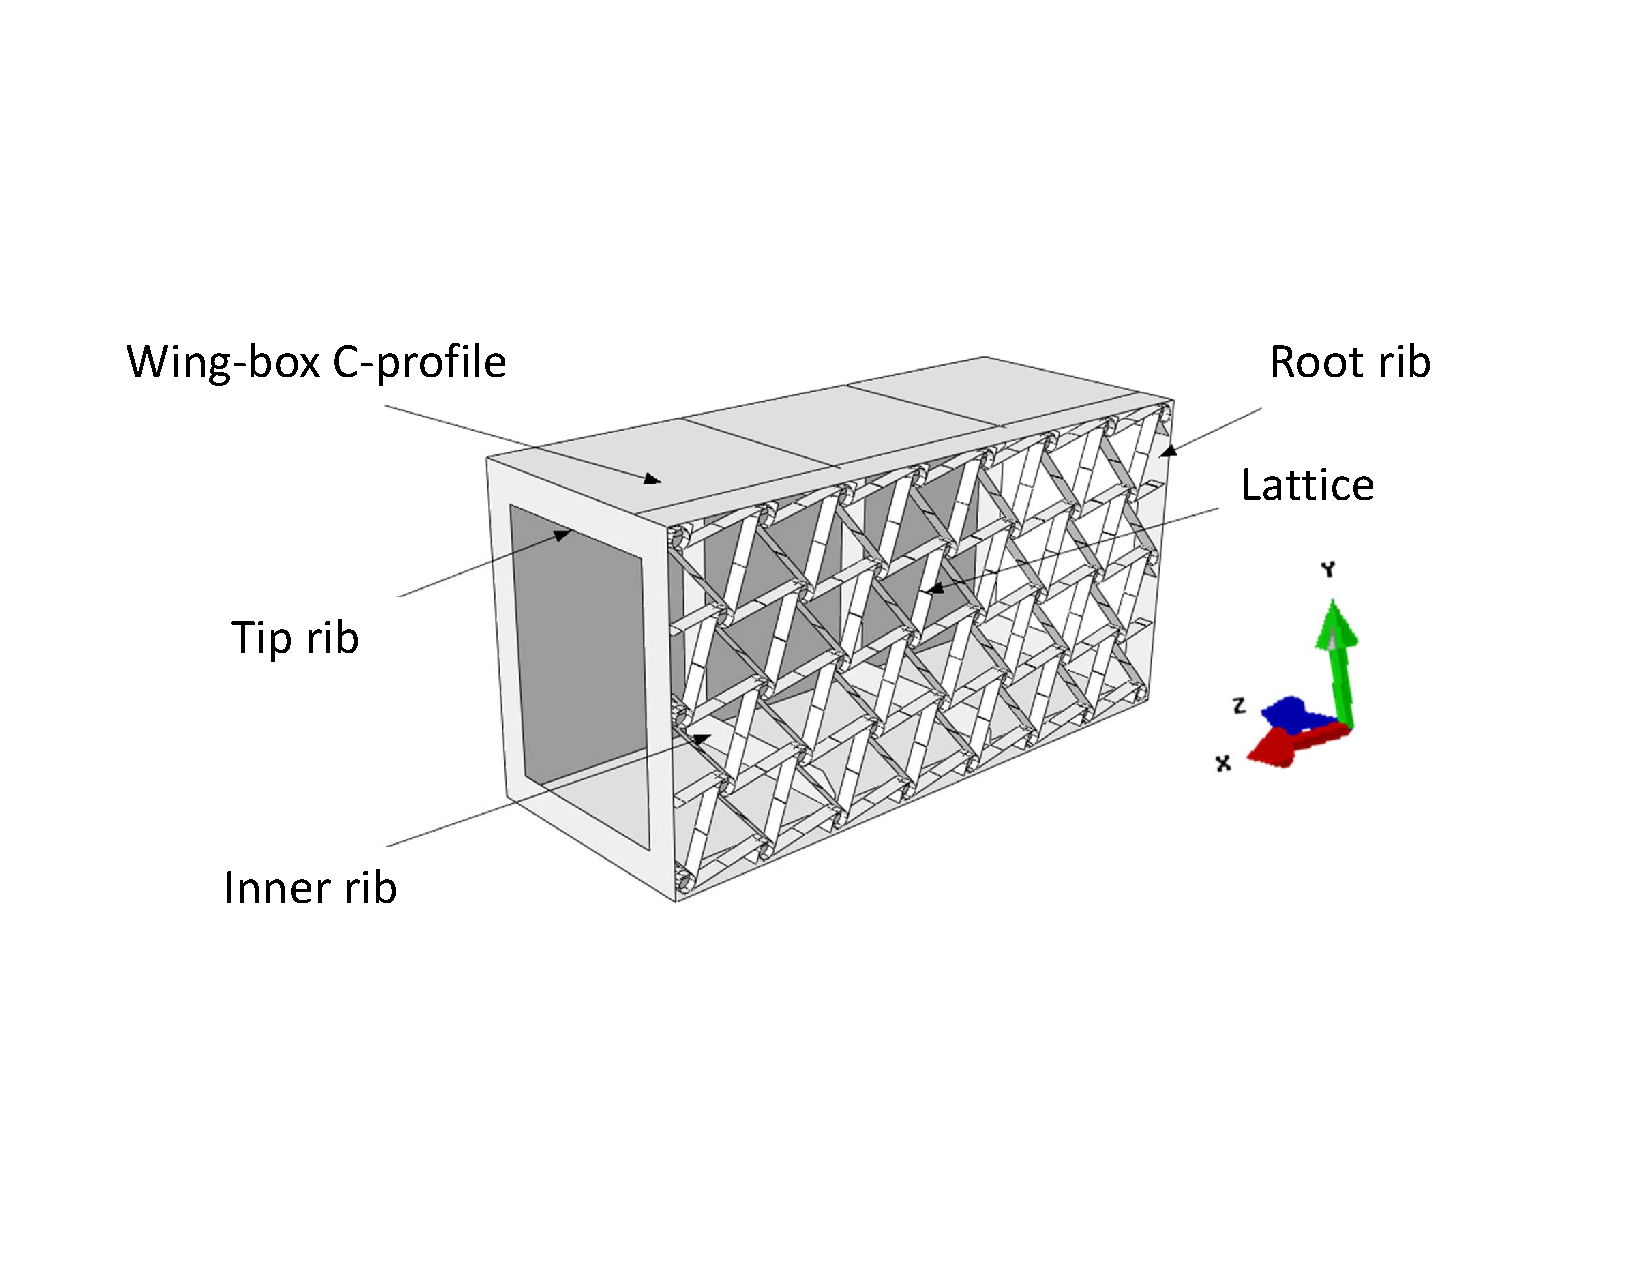
\includegraphics[width=0.8 \textwidth]{model/all-assembly}
    \caption[General assembly configuration for the computational model]{General assembly configuration for the computational model. The different parts for the general configuration include the wing-box profile, the lattice and the pair of ribs located at the tip and the root of the wing-box.}\label{fig:all-assembly}
  \end{figure}

  The discretization of the structural element was done using continuum shell elements as the basic constituting part. An sketch of a continuum shell element as defined in Abaqus can be seen in Figure \ref{fig:shellElement}.

  \begin{figure}[!htpb]
    \centering
    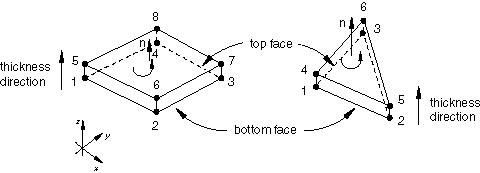
\includegraphics[width=0.8 \textwidth]{model/eshell-scon-normal-nls}
    \caption[Default normals and thickness direction for continuum shell elements in Abaqus]{Default normals and thickness direction for continuum shell elements in Abaqus. \cite{Abaqus}}\label{fig:shellElement}
  \end{figure}

  \subsection{Sub-parts and parametrization of the model} \label{subsec:parametrization_Model}

    \subsubsection{Lattice of chiral elements} \label{subsubsec:lattice_Parametrization}

    The model of the lattice structure is constituted of a series of interconnected lattices and nodes. An overview of the corresponding part can be seen in Figure \ref{fig:lattice}. The lattice structure is divided in an integer number of unit cells in the longitudinal (spanwise) and transversal directions. These parameters are identified with the variables $N$ and $M$ for the longitudinal and transversal directions, respectively. In Figure \ref{fig:lattice-NandM}, an sketch of the internal division for $N = 8$ and $M = 3$ is shown. It displays a set of horizontal rectangles that represent each of the transversal $M$ divisions while the set of vertical rectangles correspond to each of the $N$ longitudinal divisions.

    Furthermore, the internal geometry in the chiral lattices is determined by a number of parameters: the thickness $t_{\mathrm{chiral}}$, the ligament eccentricity $e_{\mathrm{chiral}}$, the ligament half length $L_{\mathrm{chiral}}$, the lattice node depth $B_{\mathrm{chiral}}$ and the lattice node radius $r_{\mathrm{chiral}}$. The geometrical meaning of these variables can be seen in Figure \ref{fig:lattice-internalParameters}. The thickness $t_{\mathrm{chiral}}$ applies for both the ligaments and the lattice nodes geometries. The eccentricity $e_{\mathrm{chiral}}$ will be expressed as the dimensionless parameter $\hat{e}_{\mathrm{chiral}}$ which is obtained from $\hat{e}_{\mathrm{chiral}} = e_{\mathrm{chiral}} / B_{\mathrm{chiral}}$.

    In the sketch shown in Figure \ref{fig:lattice-internalParameters} an additional dimension variable appears, the ligament eccentricity radius $R_{\mathrm{chiral}}$ which is dependent on the ligament eccentricity $e_{\mathrm{chiral}}$ and the lattice node depth $B_{\mathrm{chiral}}$ as shown in Equation \ref{eq:RforLattice}.

    A summary of all the parameters introduced to characterize the chiral lattice structure together with their units and nominal values is shown in Table \ref{tab:parameters_lattice}.

    \begin{equation}\label{eq:RforLattice}
      R = \frac{e_{\mathrm{chiral}}^2 + \frac{B_{\mathrm{chiral}}^2}{4}}{2e_{\mathrm{chiral}}}
    \end{equation}

    \begin{figure}[!htpb]
      \centering
      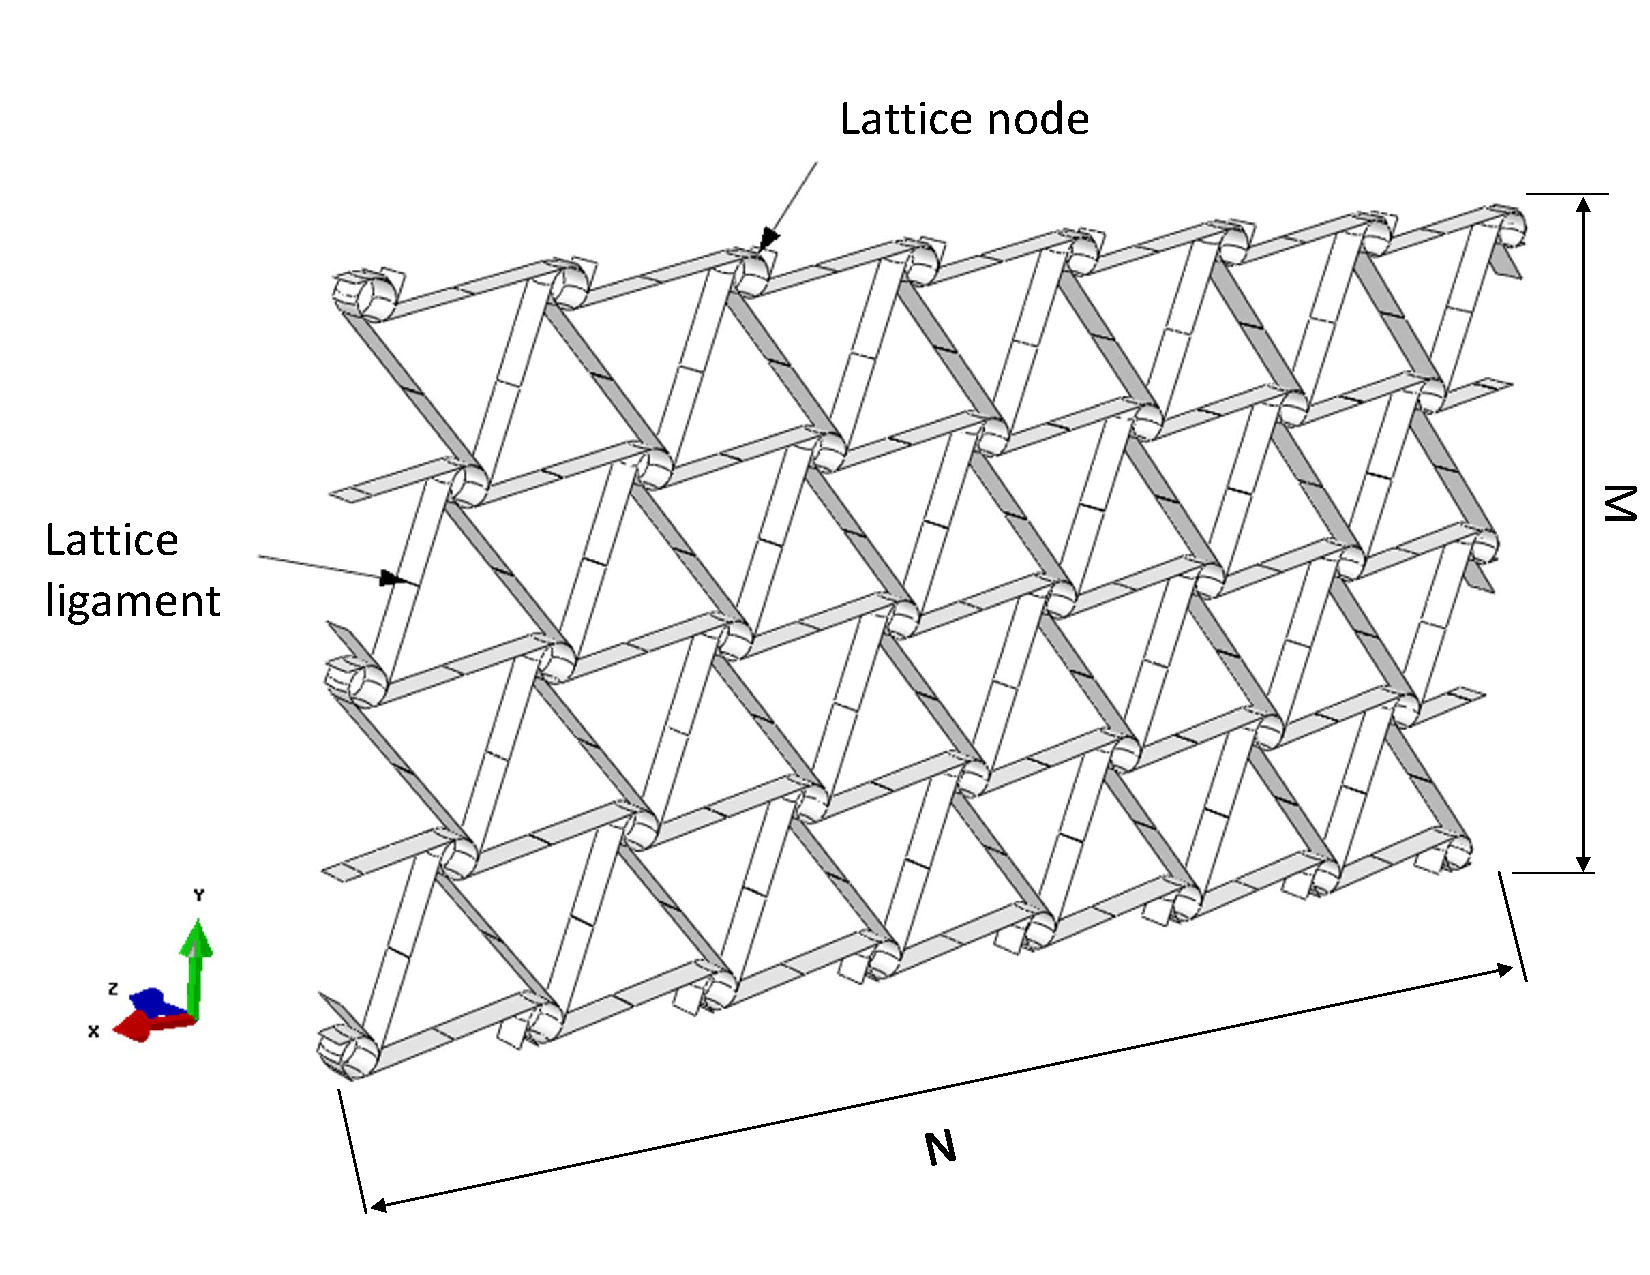
\includegraphics[width=0.8 \textwidth]{model/lattice}
      \caption[Overview of the chiral lattice part]{Overview of the chiral lattice part. The parameters $N$ and $M$ represent the number of unit cells in the longitudinal (spanwise) and transversal directions, respectively.}\label{fig:lattice}
    \end{figure}

    \begin{figure}[!htpb]
      \centering
      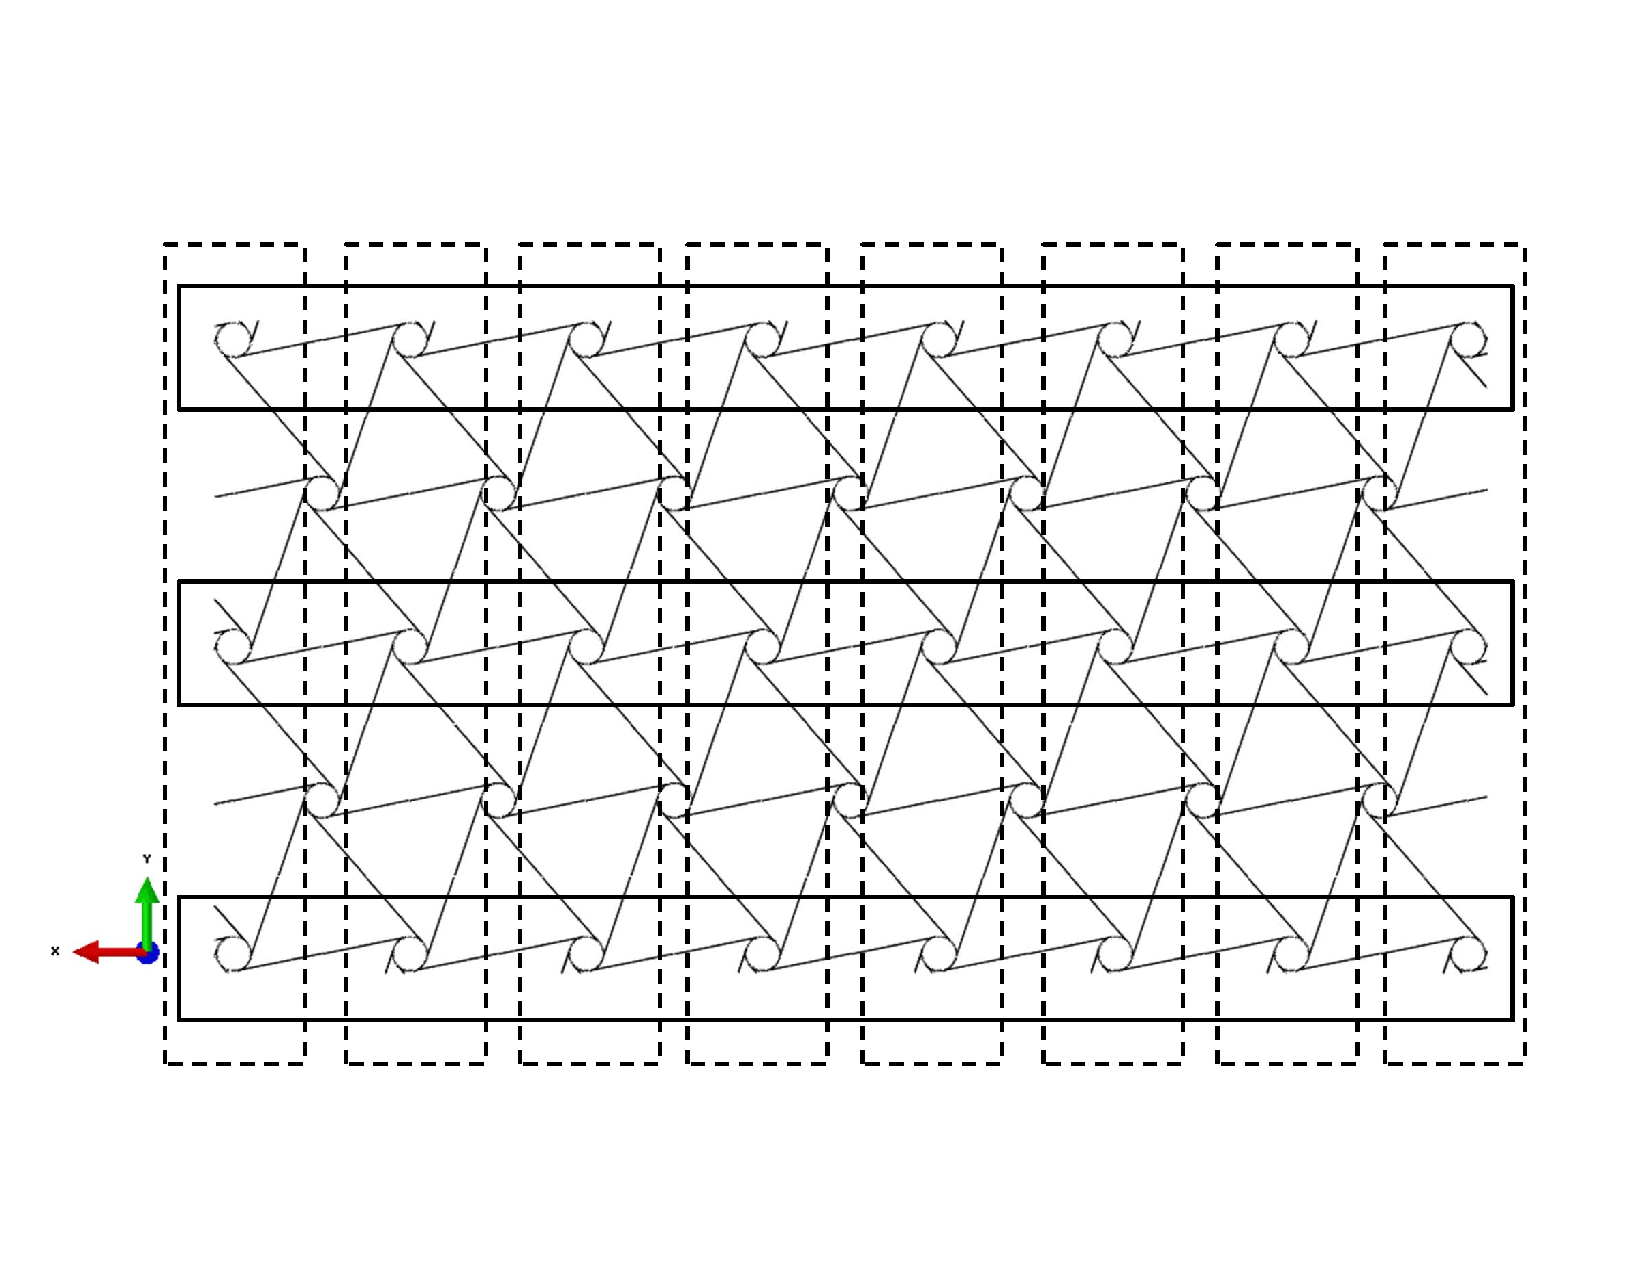
\includegraphics[width=0.8 \textwidth]{model/lattice-NandM}
      \caption[Division of the lattice structure in cell units]{Division of the lattice structure in cell units. The sketch shows a lattice with $N = 8$ and $M = 3$. The set of horizontal rectangles represent each of the transversal $M$ divisions while the set of vertical rectangles correspond to each of the $N$ longitudinal divisions.}\label{fig:lattice-NandM}
    \end{figure}

    \begin{figure}[!htpb]
      \centering
      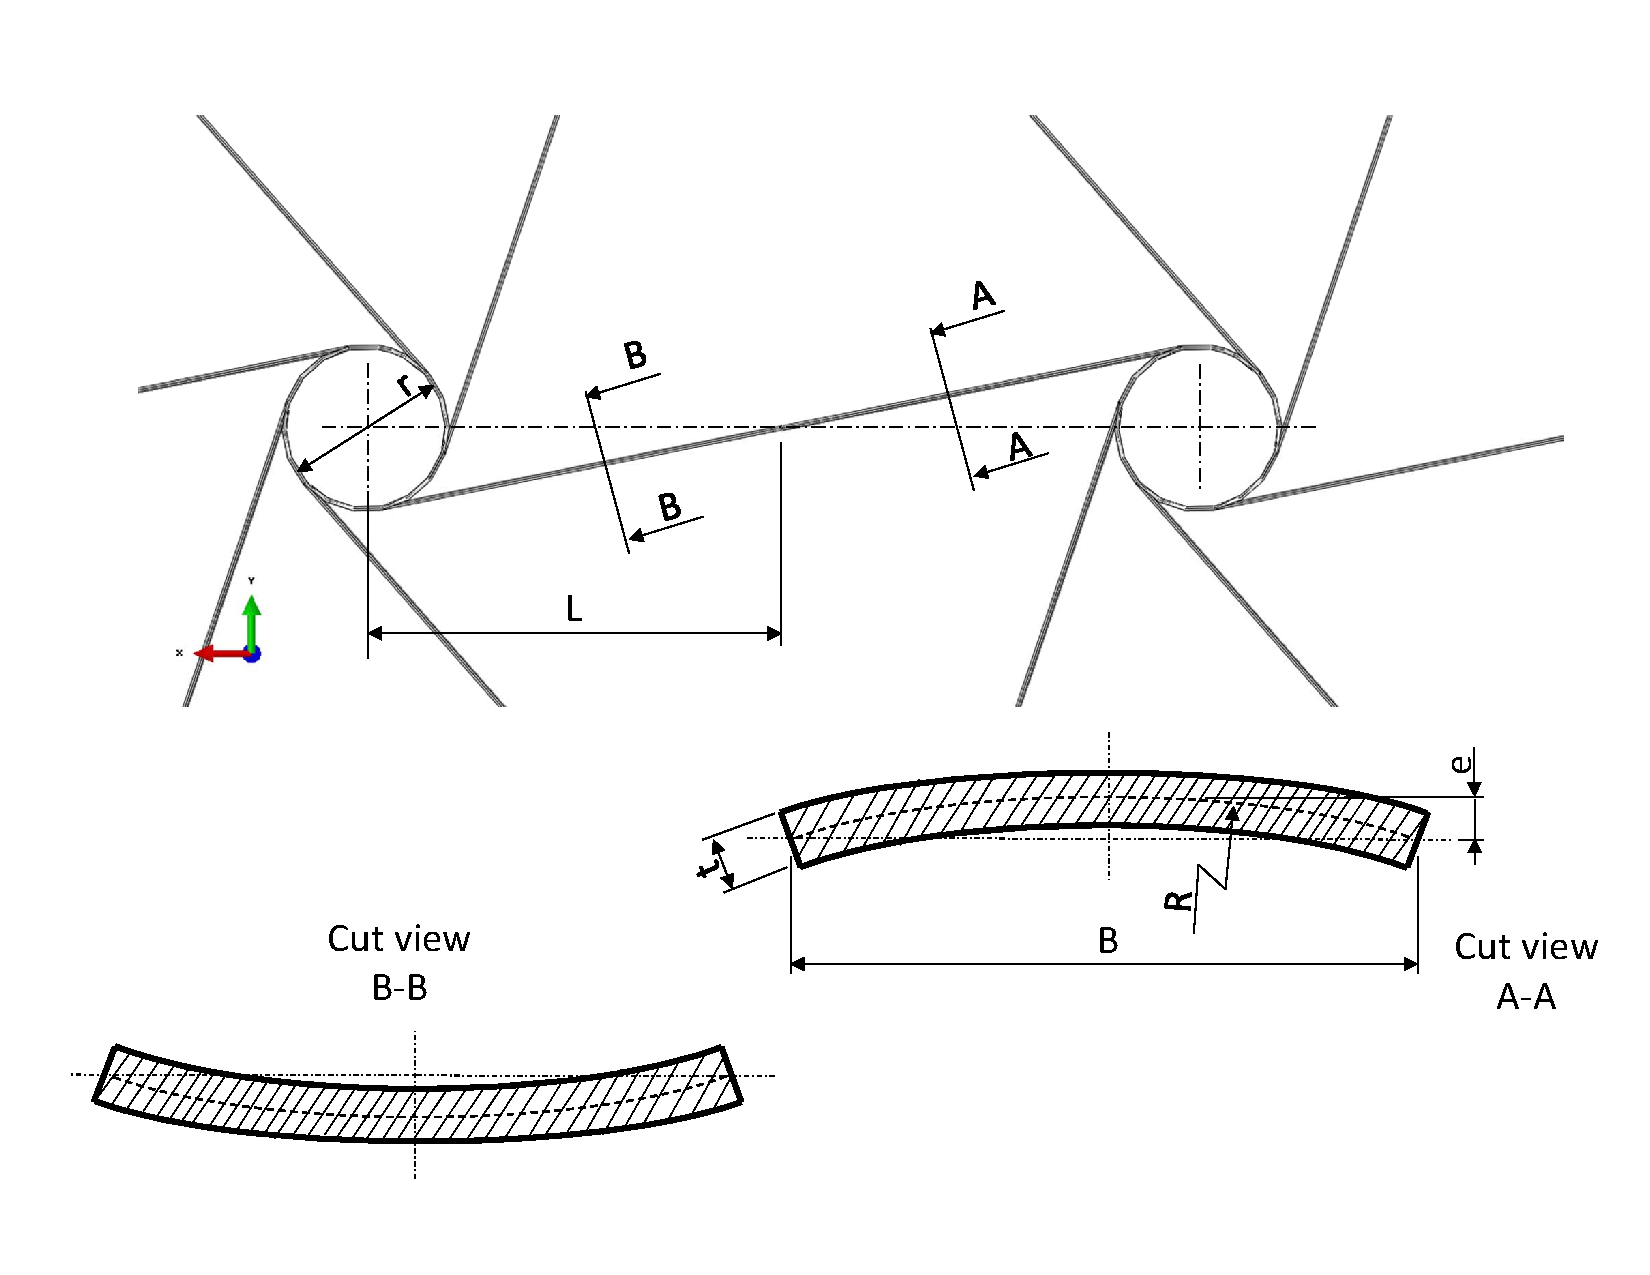
\includegraphics[width=0.8 \textwidth]{model/lattice-internalParameters}
      \caption[Internal parameters of the chiral lattice structure]{Internal parameters of the chiral lattice structure. The geometry is characterized by the the ligament eccentricity $e_{\mathrm{chiral}}$, the ligament half length $L_{\mathrm{chiral}}$, the lattice node depth $B_{\mathrm{chiral}}$, the lattice node radius $r_{\mathrm{chiral}}$ and the thickness $t_{\mathrm{chiral}}$. The ligament eccentricity radius $R_{\mathrm{chiral}}$ which is dependent on the ligament eccentricity $e_{\mathrm{chiral}}$ and the lattice node depth $B_{\mathrm{chiral}}$, as shown in Equation \ref{eq:RforLattice}}\label{fig:lattice-internalParameters}
    \end{figure}

    \begin{table}[!htpb]
    \centering
    \begin{tabular}{|l|lll|}
    \hline
    \textbf{Parameter} & \multicolumn{1}{l|}{\textbf{Symbol}} & \multicolumn{1}{l|}{\textbf{Units}} & \textbf{Nominal value} \\ \hline \hline
    {\textbf{Dimensions}} &  &  &  \\ \hline
    Number of unit cells in spanwise direction & \multicolumn{1}{l|}{$N$} & \multicolumn{1}{l|}{} & 8 \\ \hline
    Number of unit cells in transversal direction & \multicolumn{1}{l|}{$M$} & \multicolumn{1}{l|}{} & 3 \\ \hline
    Dimensionless ligament eccentricity (e/B) & \multicolumn{1}{l|}{$\hat{e}_{\mathrm{chiral}}$} & \multicolumn{1}{l|}{} & 0.01 \\ \hline
    Node radius & \multicolumn{1}{l|}{$r_{\mathrm{chiral}}$} & \multicolumn{1}{l|}{mm} & 10 \\ \hline
    Node depth & \multicolumn{1}{l|}{$B_{\mathrm{chiral}}$} & \multicolumn{1}{l|}{mm} & 20 \\ \hline
    Ligament eccentricity radius & \multicolumn{1}{l|}{$R_{\mathrm{chiral}}$} & \multicolumn{1}{l|}{mm} & 250.1 \\ \hline
    Ligament half length & \multicolumn{1}{l|}{$L_{\mathrm{chiral}}$} & \multicolumn{1}{l|}{mm} & 50 \\ \hline
    Thickness & \multicolumn{1}{l|}{$t_{\mathrm{chiral}}$} & \multicolumn{1}{l|}{mm} & 0.5 \\ \hline \hline
    {\textbf{Material (ABS)}} &  &  &  \\ \hline
    Young's modulus & \multicolumn{1}{l|}{$E_{\mathrm{chiral}}$} & \multicolumn{1}{l|}{N/mm$^2$} & 3100 \\ \hline
    Poisson's ratio & \multicolumn{1}{l|}{$\nu_{\mathrm{chiral}}$} & \multicolumn{1}{l|}{} & 0.3 \\ \hline
    \end{tabular}
    \caption[Parameters used for the lattice model]{Parameters used for the lattice model. The mechanical properties of the material used correspond to ABS, which is a common thermoplastic polymer.}
    \label{tab:parameters_lattice}
    \end{table}

    %This is like if it was a new section inside of this section
    \clearpage
    \subsubsection{Lattice nodes rigid body modeling} \label{subsubsec:latticeNodesRigid_Parametrization}

    The lattice nodes is one of the essential parts of the lattice of chiral elements. These are allow to freely rotate around its own axis. For the modeling, they are assumed to behave like a rigid body. In Figure \ref{fig:closeLookToLatticeNodes}, a closer look to the chiral nodes can be seen, showing two different approaches to manufacture a node that would behave like a rigid body compared with the rest of the structure.

    \begin{figure}[!htpb]
      \centering
      \includegraphics[width=0.8 \textwidth]{model/closeLookToLatticeNodes}
      \caption[Pictured of the manufactured chiral lattice nodes]{Pictured of the manufactured chiral lattice nodes. The figures shows two different approaches followed to manufacture the nodes. The one on the right was the standard one showing a cylinder with a thickness bigger than the thickness of the chiral ligaments $t_{\mathrm{node}} \gg t_{\mathrm{ligaments}}$. On the left, an alternative approach is followed in order to allow the assembly of the chiral lattice that is not manufactured as a unique piece. \cite{Vincenz2017}}\label{fig:closeLookToLatticeNodes}
    \end{figure}

    In the Abaqus model, different approaches were followed to create this element of the chiral lattice. The first one was to create a coupling condition using Abaqus corresponding module. In particular, a kinematic coupling was establish. A kinematic coupling constrains the motion of one or more coupling nodes, also called slave node or nodes, to the rigid body motion of a reference node, also called master node. They are imposed by eliminating degrees of freedom at the coupling nodes. In Figure \ref{fig:kinematicCoupling}, an example of a kinematic coupling can be seen.

    \begin{figure}[!htpb]
      \centering
      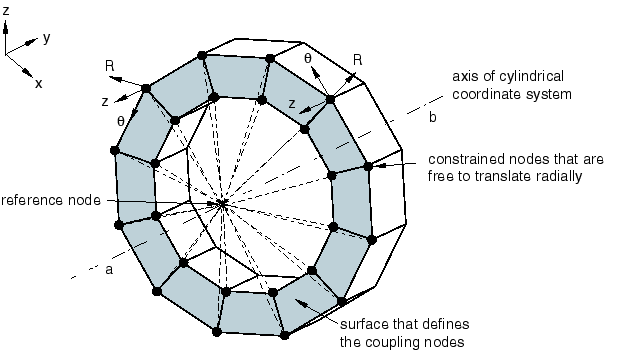
\includegraphics[width=0.8 \textwidth]{model/pcoupling-kinematic}
      \caption[Kinematic coupling constraint]{Kinematic coupling constraint. The sketch illustrates the use of a kinematic coupling constraint to prescribe a twisting motion to a model without constraining the radial motion. In this case, a local cylindrical reference system is used and the constrained nodes have two degrees of freedom coupled to those of the reference node, the angular position $\theta$ and the position along the $z$ axis. The coupling nodes are therefore free to translate radially, varying $R$. \cite{Abaqus}}\label{fig:kinematicCoupling}
    \end{figure}

    For the considered case, the coupling nodes are those mesh nodes located faces of the lattice node and the master node is the reference point located in the center of the lattice node. In order to achieve the rigid solid behavior, all the degrees of freedom were coupled except from the translation displacements in the plane where the chiral lattice is contained, i.e. the translational displacement $U_1$ and $U_2$ of the plane $X-Y$. In Figure \ref{fig:couplingThroughRF} an overview of this coupling condition can be viewed.

    \begin{figure}[!htpb]
      \centering
      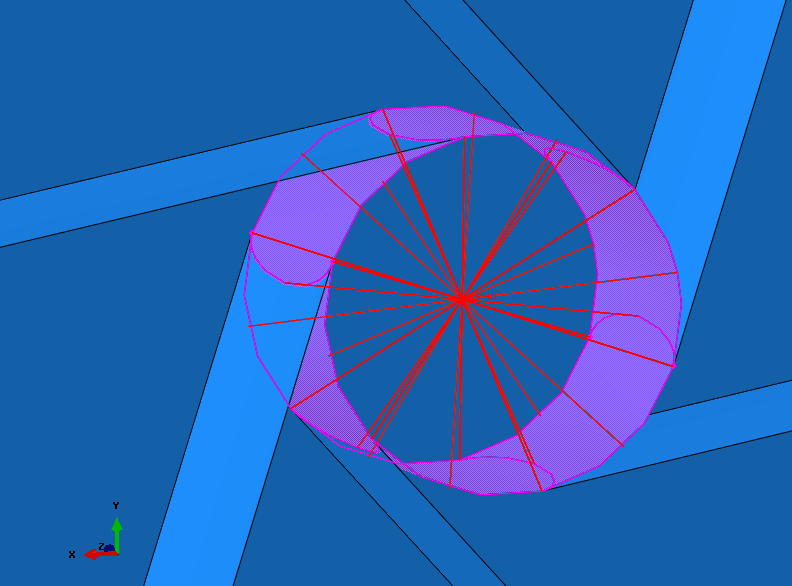
\includegraphics[width=0.8 \textwidth]{model/couplingThroughRF}
      \caption[Overview of the elements that are involved in the coupling condition at the lattice nodes]{Overview of the elements that are involved in the coupling condition at the lattice nodes. The coupling condition was defined in between the mesh nodes located in the faces of the lattince node and a reference point located in the middle. All the degrees of fredom were linked except from the translation displacements in the plane where the chiral lattice is contained, i.e. the translational displacement $U_1$ and $U_2$ of the plane $X-Y$.}\label{fig:couplingThroughRF}
    \end{figure}

    Another approach consisted in inserting an addition part inside the lattice nodes to add rigidity to the element. The proposed design of such a part, which will be referred as tyre from now on, can be seen in Figure \ref{fig:tyre-part}. The internal dimensions of this element are shown in Figure \ref{fig:tyre-internalParameters}. This dimensions were dependent on parameters of the chiral lattice. In other words, the thickness of the tyre was equal to that of the chiral lattice $r_{\mathrm{tyre}} = r_{\mathrm{chiral}}$ and the same occurred for the height $B_{\mathrm{tyre}}$ and the radius $r_{\mathrm{tyre}}$ which were $r_{\mathrm{tyre}} = r_{\mathrm{chiral}}$ and $B_{\mathrm{tyre}} = B_{\mathrm{chiral}}$. The added rigidity was obtained as a result of considering a different material for the tyre such that the Young's modulus of the two parts verify the condition $E_{\mathrm{tyre}} \gg E_{\mathrm{chiral}}$. Once, the connection was completed, the resulting merged part looked as shown in Figure \ref{fig:tyre-connection}.

    \begin{figure}[!htpb]
      \centering
      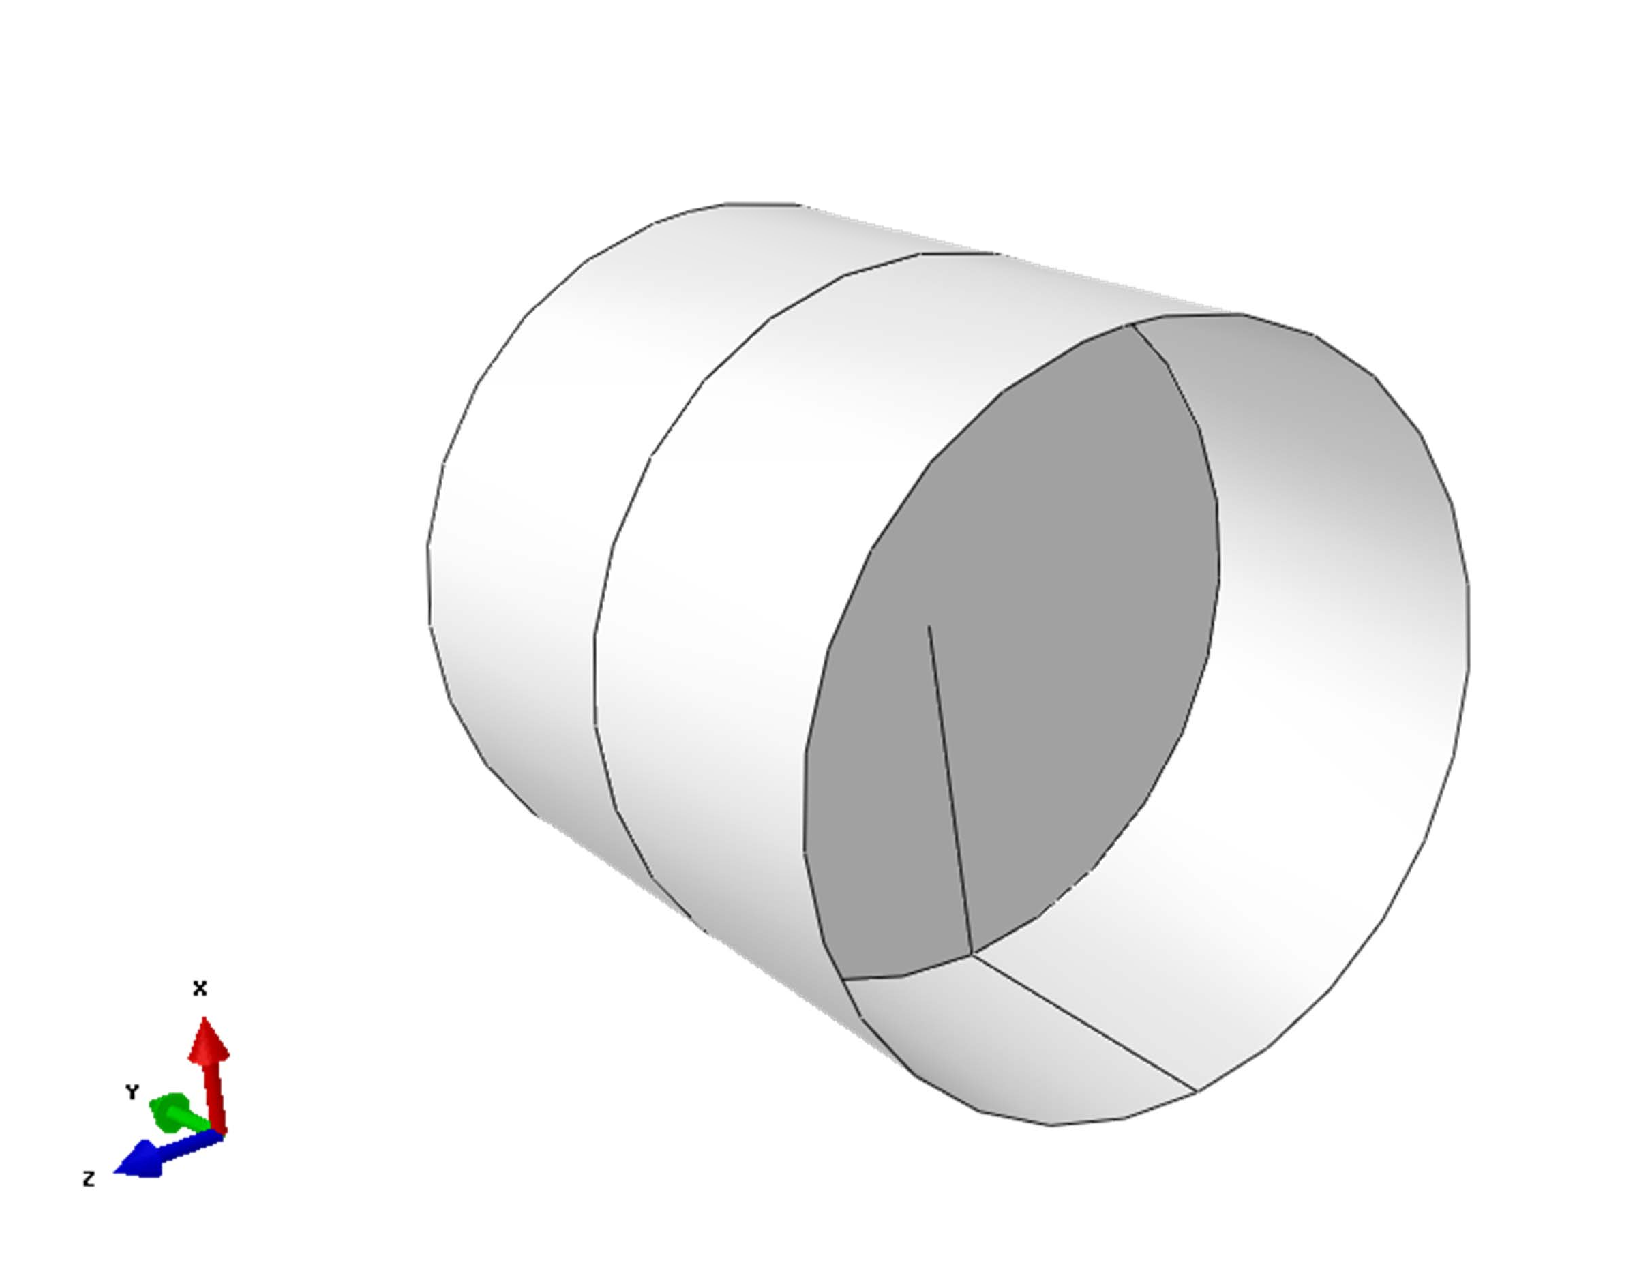
\includegraphics[width=0.8 \textwidth]{model/tyre-part}
      \caption[Overview of the tyre part]{Overview of the tyre part.}\label{fig:tyre-part}
    \end{figure}

    \begin{figure}[!htpb]
      \centering
      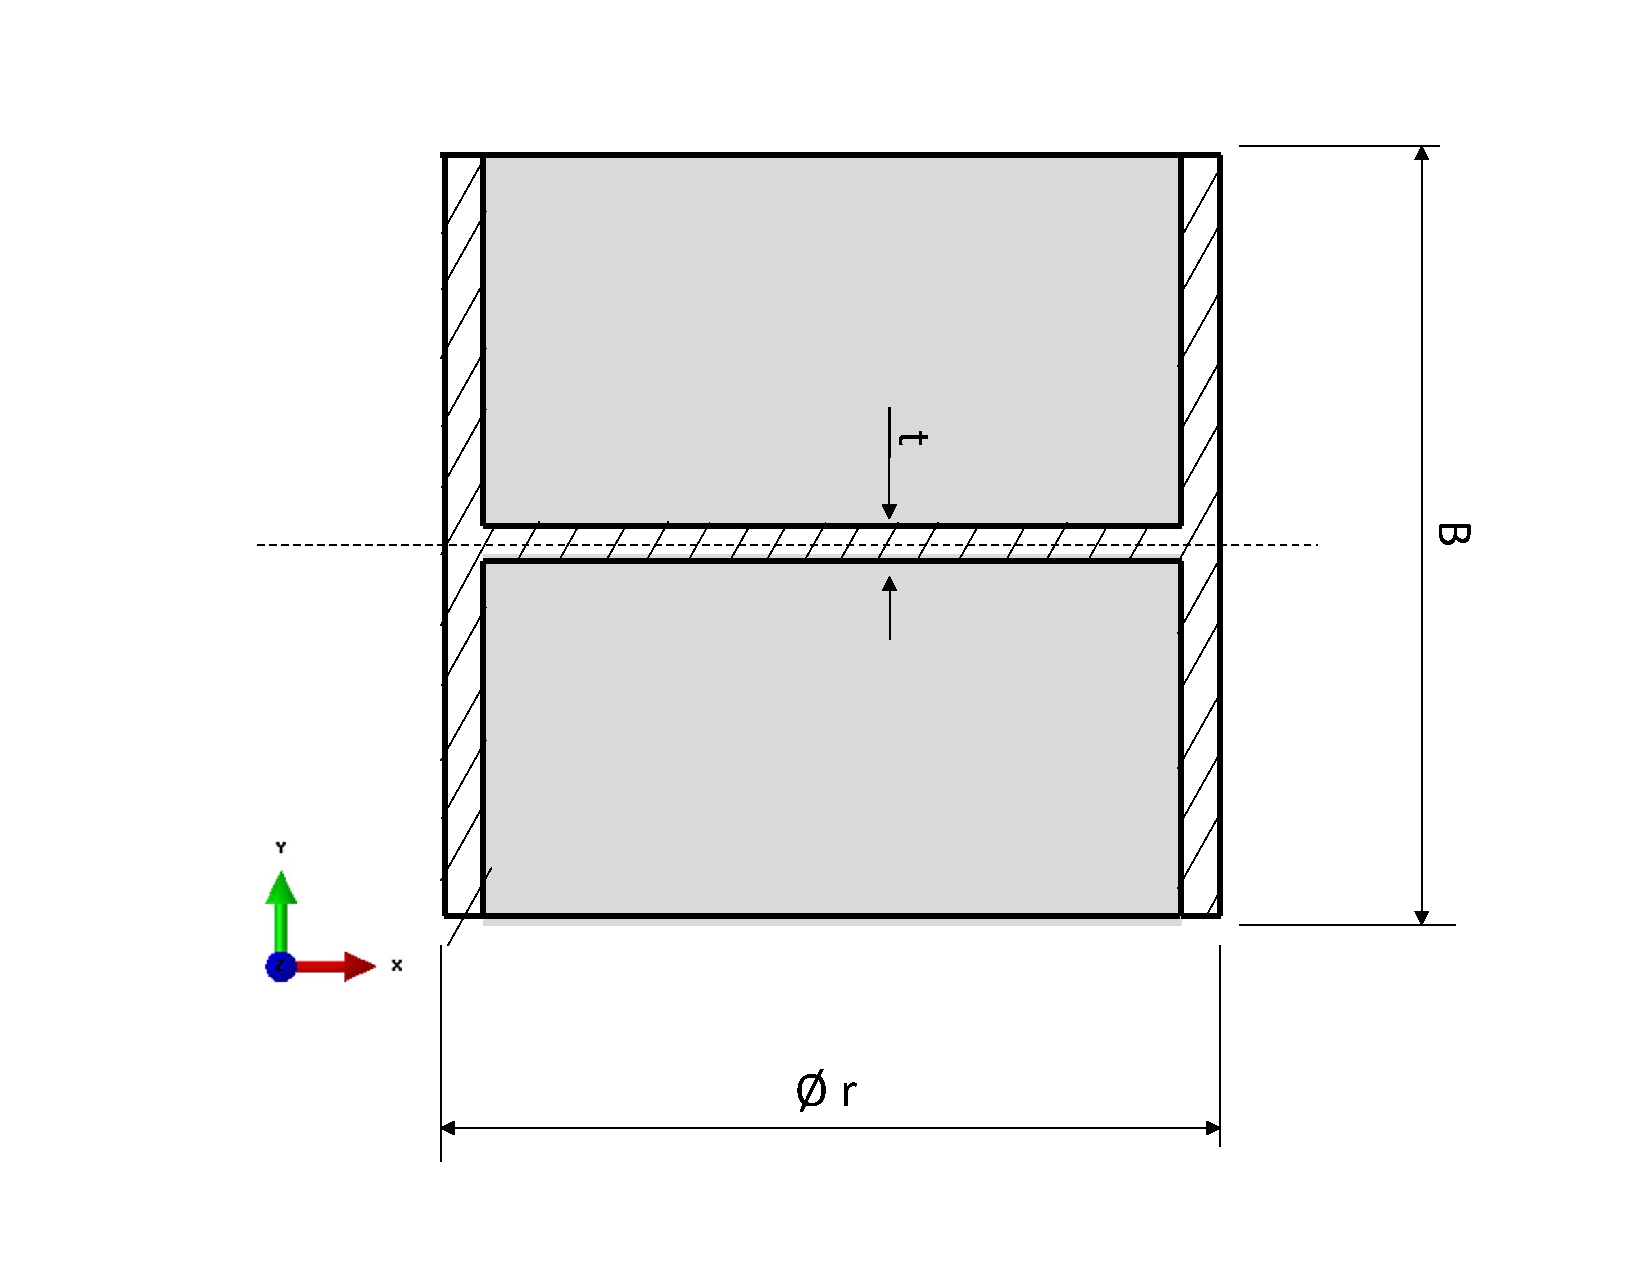
\includegraphics[width=0.8 \textwidth]{model/tyre-internalParameters}
      \caption[Internal parameters of the tyre part]{Internal parameters of the tyre part. The sketch shows a transversal cut to the part. The tyre is characterized by the radius $r_{\mathrm{tyre}}$, the height $B_{\mathrm{tyre}}$ and the thickness $t_{\mathrm{tyre}}$. All this parameters were equal to the corresponding ones in the lattice nodes, therefore: $r_{\mathrm{tyre}} = r_{\mathrm{chiral}}$, $B_{\mathrm{tyre}} = B_{\mathrm{chiral}}$ and $t_{\mathrm{tyre}} = t_{\mathrm{chiral}}$.}\label{fig:tyre-internalParameters}
    \end{figure}

    \begin{figure}[!htpb]
      \centering
      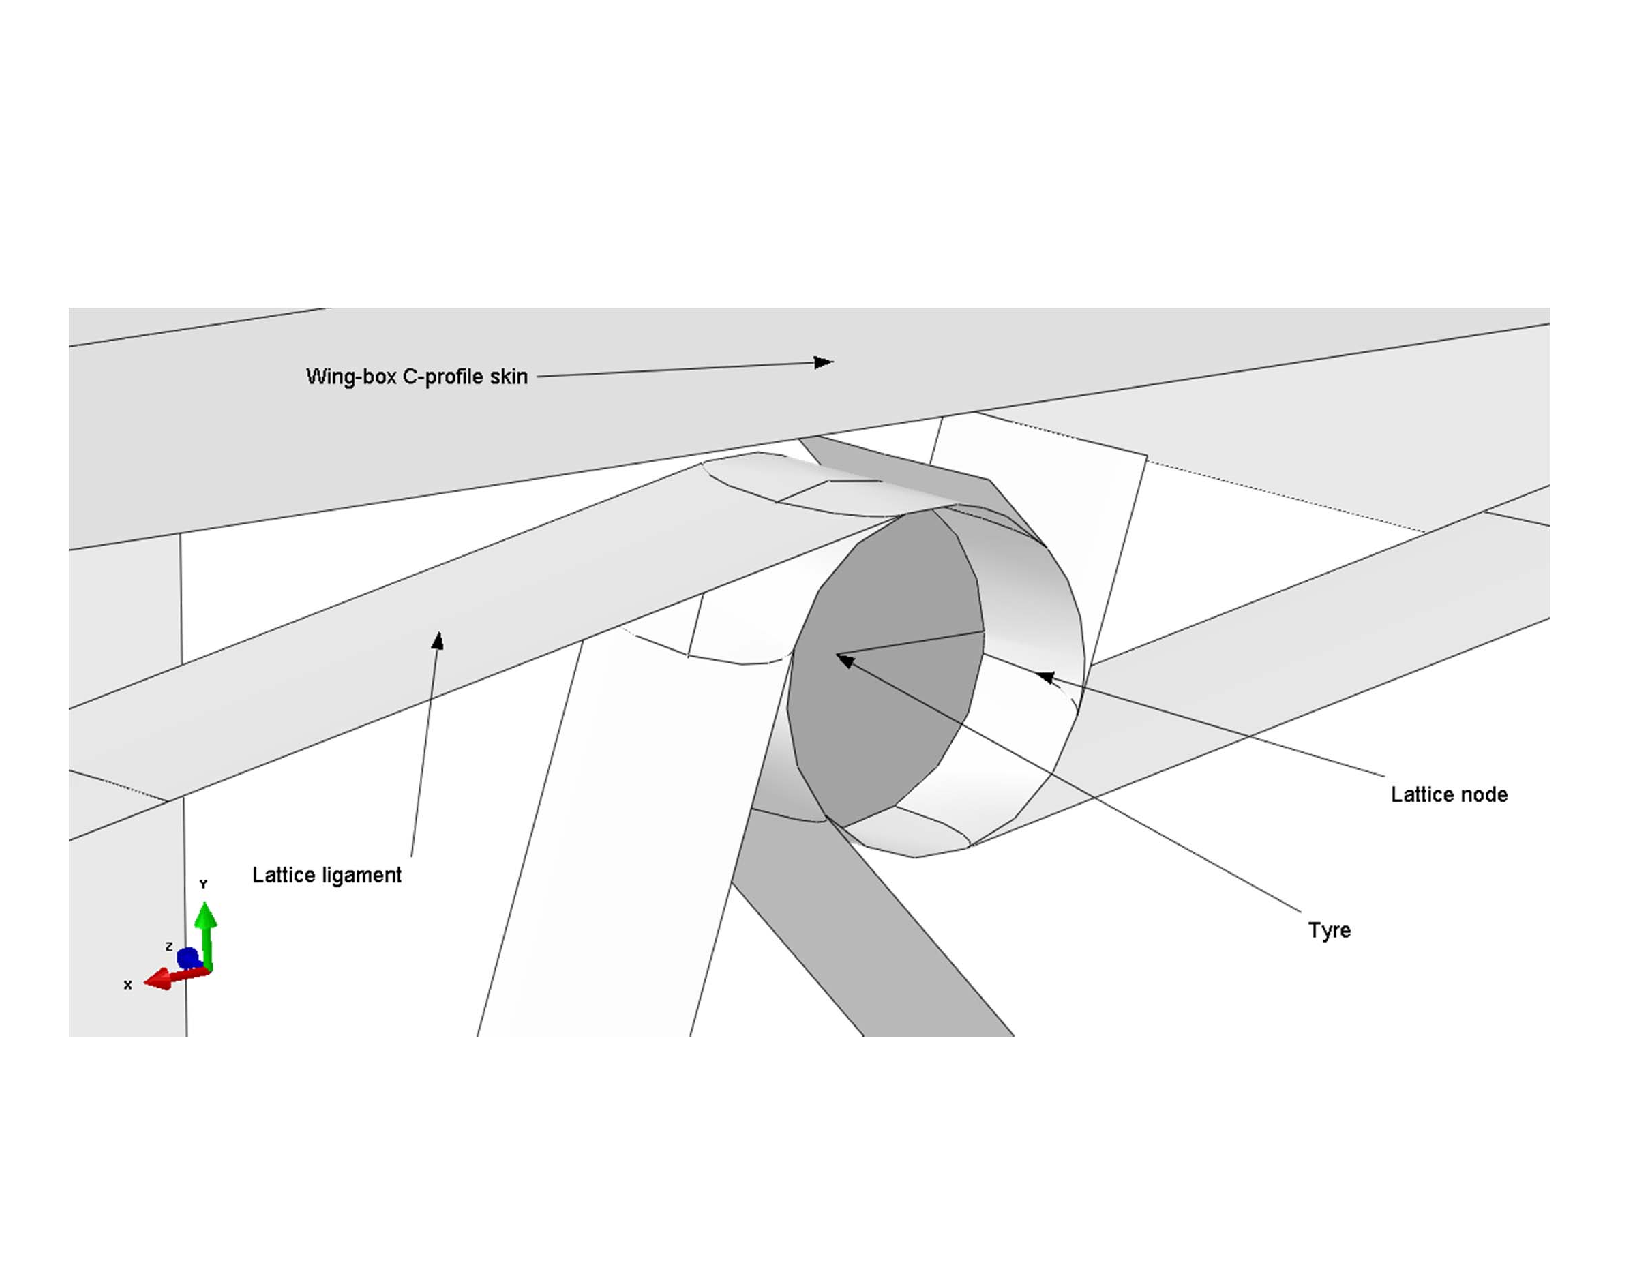
\includegraphics[width=0.8 \textwidth]{model/tyre-connection}
      \caption[Overview of the connection between tyre and lattice node]{Overview of the connection between tyre and lattice node. The tyre will be embed inside the lattice node.}\label{fig:tyre-connection}
    \end{figure}

    \clearpage
    \subsubsection{Wing-box in C-profile} \label{subsubsec:wingBox_Parametrization}

    %Description of the wing box
    The model of the wing-box consisted on a beam with open C profile. The length $L_{\mathrm{box}}$ and height $H_{\mathrm{box}}$ of the part were determined from those of the lattice of chiral elements. Therefore, the tailorable parameters for this part are the width $W_{\mathrm{box}}$, the thickness $t_{\mathrm{box}}$ and the mechanical properties $E_{\mathrm{box}}$ and $\nu_{\mathrm{box}}$ of the material used. The value of the Wing-box height $H_{\mathrm{box}}$ and the wing-box length $L_{\mathrm{box}}$ are not independent but are calculated based on the transversal and longitudinal dimensions of the chiral lattice structure, respectively.

    \begin{figure}[!htpb]
      \centering
      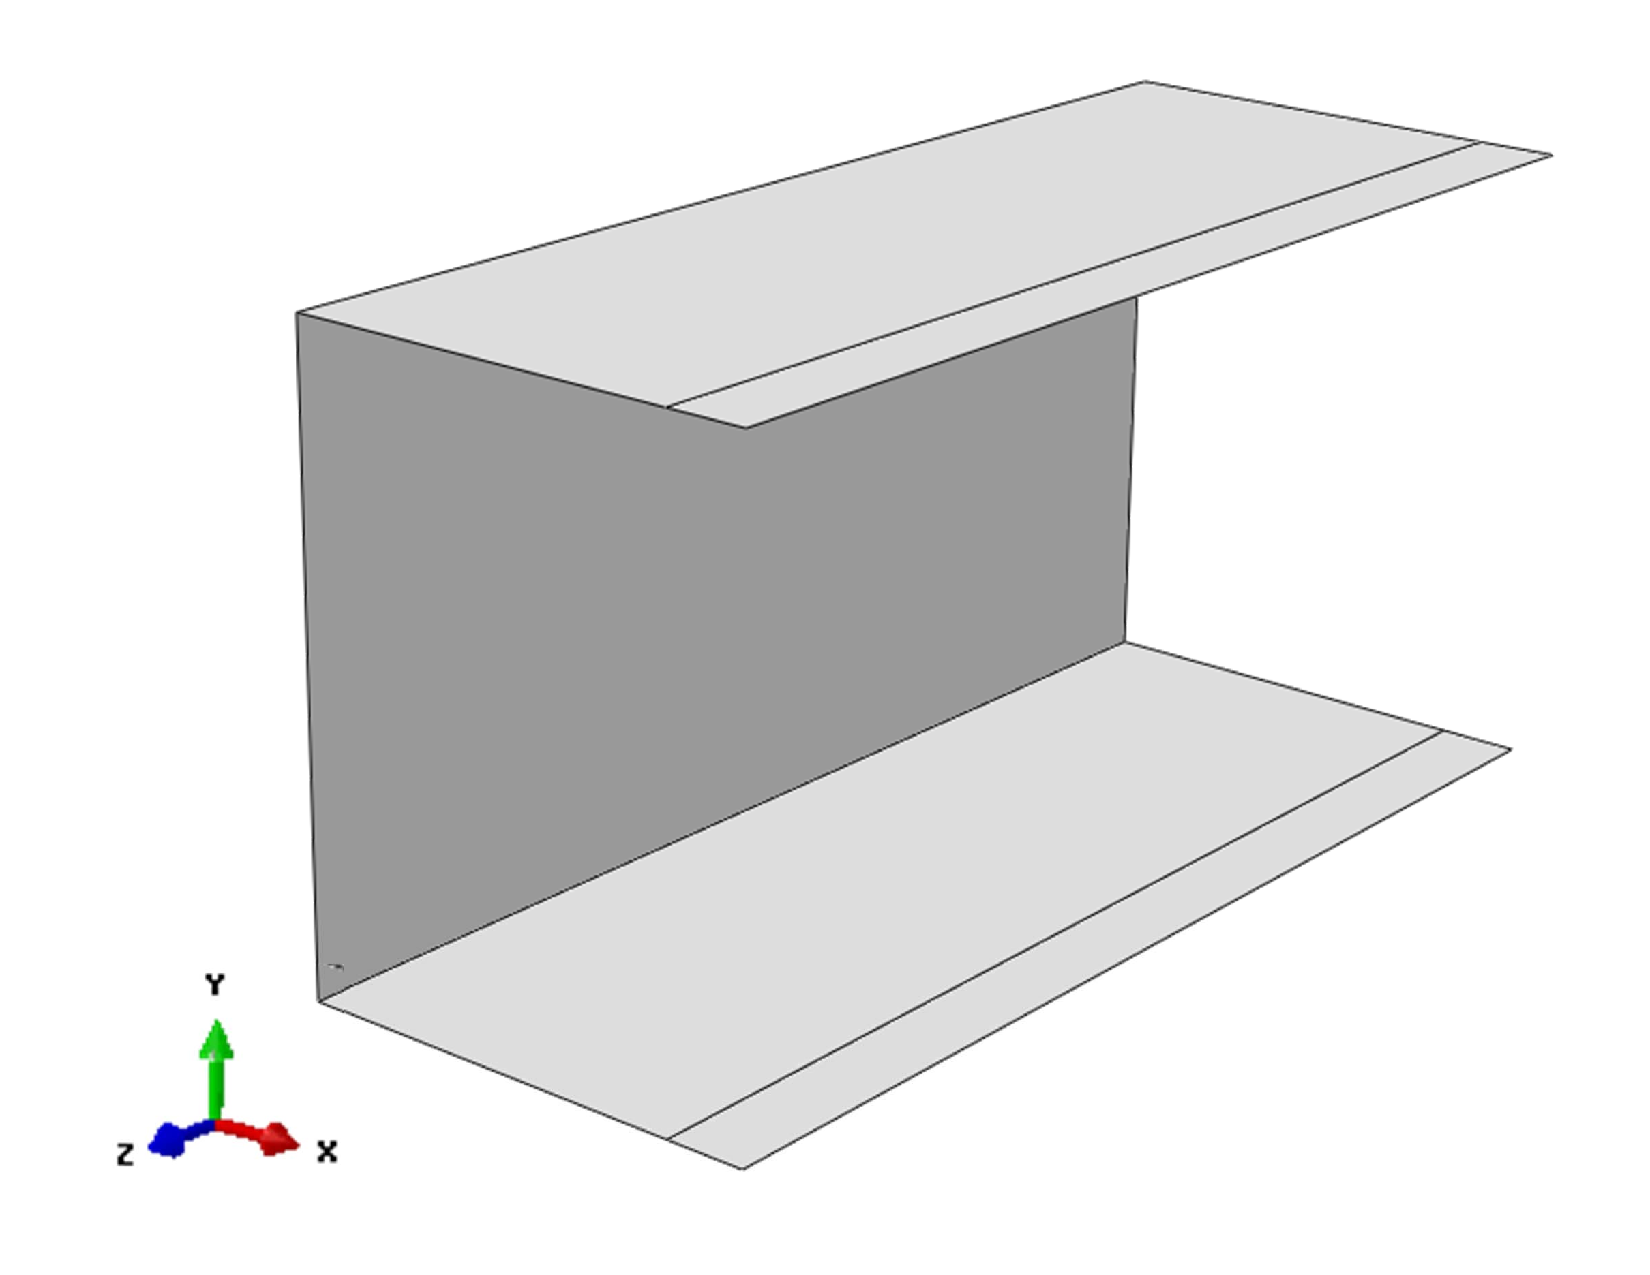
\includegraphics[width=0.8 \textwidth]{model/wing-box}
      \caption[Overview of the wing-box in C-profile part]{Overview of the wing-box in C-profile part}\label{fig:wing-box}
    \end{figure}

    In the sketch shown in Figure \ref{fig:wing-box-internalParameters} it is possible see the geometrical meaning of the parameters introduced in the previous paragraph. Additionally, the Table \ref{tab:parameters_wing-box} shows its units and nominal values.

    \begin{figure}[!htpb]
      \centering
      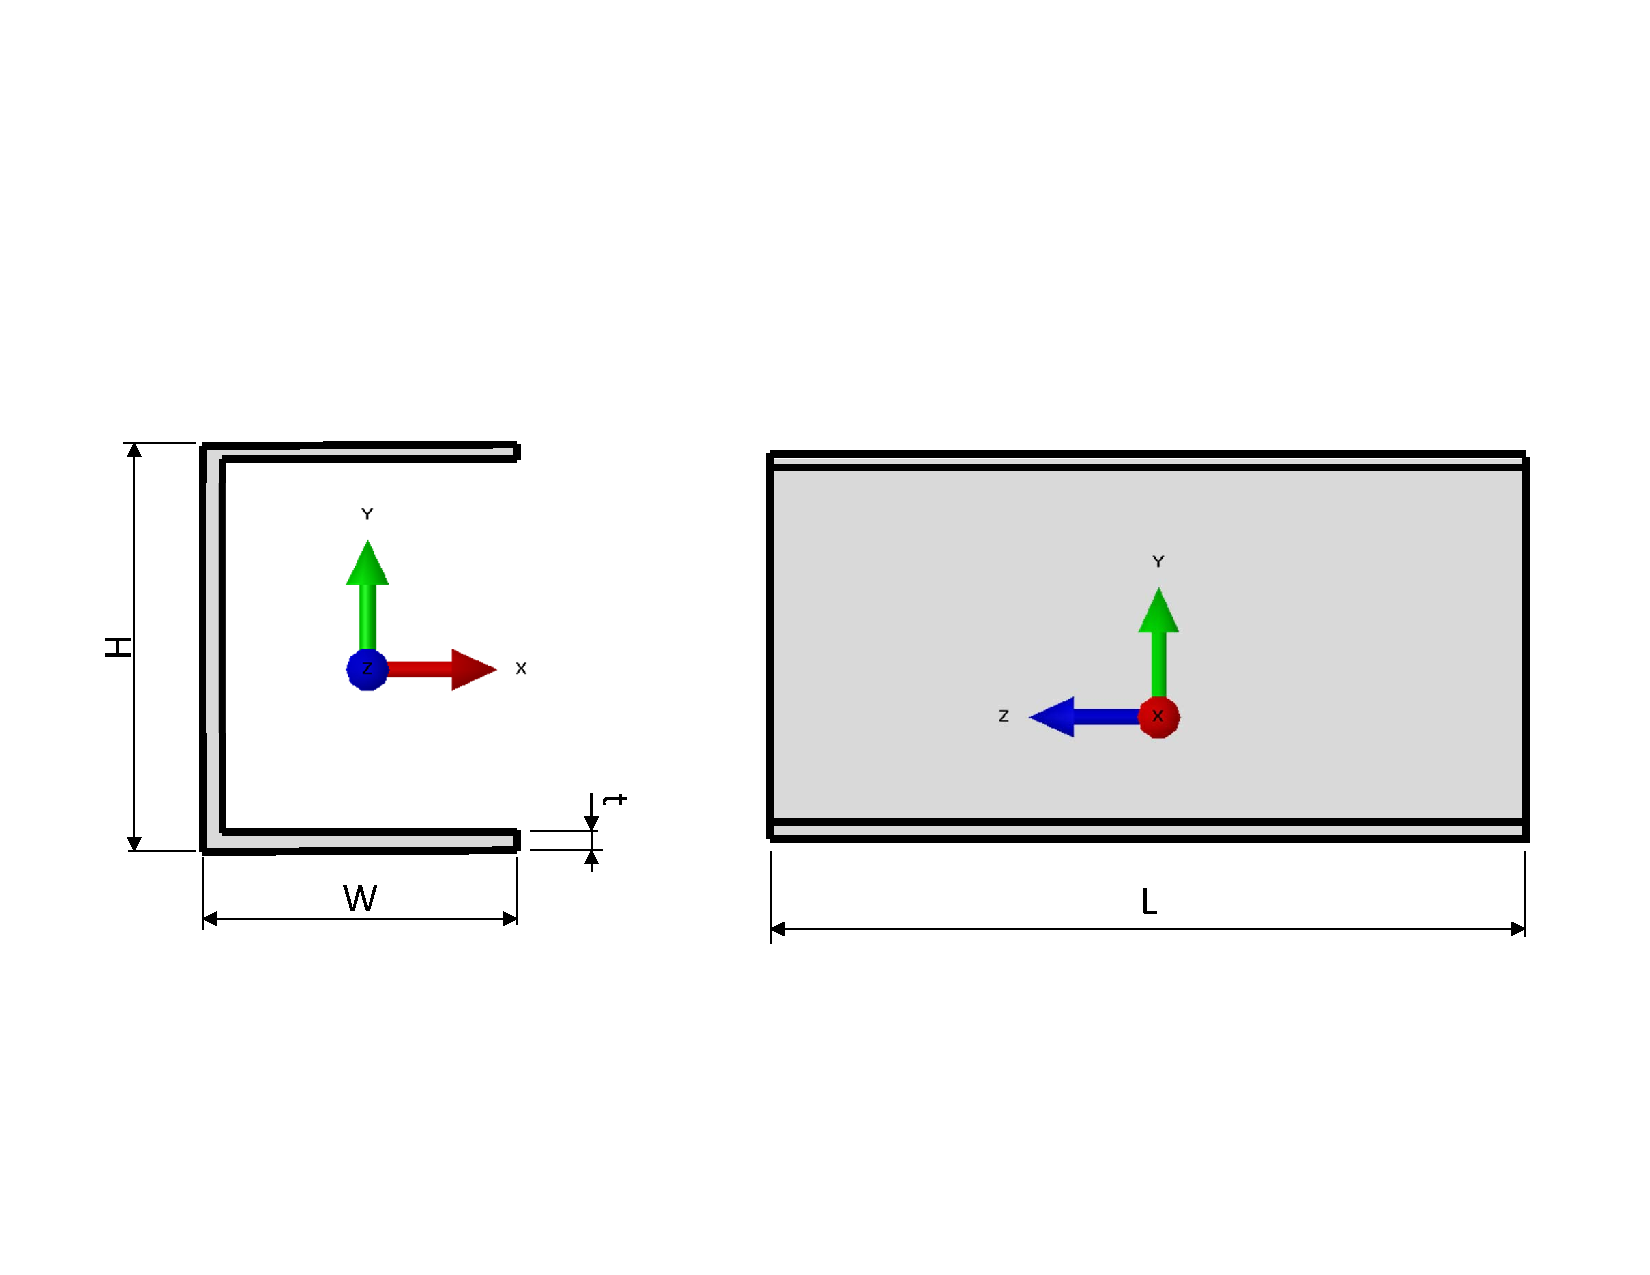
\includegraphics[width=0.8 \textwidth]{model/wing-box-internalParameters}
      \caption[Internal parameters of the wing-box in C-profile part]{Internal parameters of the wing-box C-profile part. The geometry of the part is determined by the length $L_{\mathrm{box}}$, height $H_{\mathrm{box}}$ and the width $W_{\mathrm{box}}$. Additionally, the thickness $t_{\mathrm{box}}$ is measured in the $z$ direction.}\label{fig:wing-box-internalParameters}
    \end{figure}

    \begin{table}[!htpb]
    \centering
    \begin{tabular}{|l|lll|}
    \hline
    \textbf{Parameter} & \multicolumn{1}{l|}{\textbf{Symbol}} & \multicolumn{1}{l|}{\textbf{Units}} & \textbf{Nominal value} \\ \hline \hline
    {\textbf{Dimensions}} &  &  &  \\ \hline
    Wing-box height & \multicolumn{1}{l|}{$H_{\mathrm{box}}$} & \multicolumn{1}{l|}{mm} & 383.27 \\ \hline
    Wing-box length & \multicolumn{1}{l|}{$L_{\mathrm{box}}$} & \multicolumn{1}{l|}{mm} & 743.86 \\ \hline
    Wing-box width & \multicolumn{1}{l|}{$W_{\mathrm{box}}$} & \multicolumn{1}{l|}{mm} & 300 \\ \hline
    Wing-box thickness & \multicolumn{1}{l|}{$t_{\mathrm{box}}$} & \multicolumn{1}{l|}{mm} & 0.8 \\ \hline \hline
    {\textbf{Material (Aluminum)}} &  &  &  \\ \hline
    Young's modulus & \multicolumn{1}{l|}{$E_{\mathrm{box}}$} & \multicolumn{1}{l|}{N/mm$^2$} & 69000 \\ \hline
    Poisson's ratio & \multicolumn{1}{l|}{$\nu_{\mathrm{box}}$} & \multicolumn{1}{l|}{} & 0.3269 \\ \hline
    \end{tabular}
    \caption[Parameters used for the wing-box in C-profile model]{Parameters used for the wing-box in C-profile model. The mechanical properties of the material used correspond to standard aluminum. The value of the wing-box height $H_{\mathrm{box}}$ and the wing-box length $L_{\mathrm{box}}$ are not independent but are calculated based on the transversal and longitudinal dimensions of the chiral lattice structure, respectively.}
    \label{tab:parameters_wing-box}
    \end{table}

    \clearpage
    \subsubsection{Ribs} \label{subsubsec:Ribs_Parametrization}

    As it was shown in Figure \ref{fig:all-assembly}, there are two possible ribs that can be added to the model assembly. This will add rigidity to the wing-box. The ribs located at the tip and at the root will have a closed section, similar to a frame with width $A_{\mathrm{rib}}$. The width $W_{\mathrm{rib,close}}$ and the height $H_{\mathrm{rib}}$ will be equal to the wing-box width $W_{\mathrm{box}}$ and to the chiral lattice structure height, respectively. The thickness will be $t_{\mathrm{rib}}$.

    The inner ribs will present an open section with same height $H_{\mathrm{rib}}$ and thickness $t_{\mathrm{rib}}$ as the closed configuration but different width $W_{\mathrm{rib,open}}$. The value of $W_{\mathrm{rib,open}}$ is calculated as follows:
    $$
    W_{\mathrm{rib,open}} = B_{\mathrm{chiral}} + W_{\mathrm{rib,close}} + d_{\mathrm{chiral-rib}}
    $$
    where $d_{\mathrm{chiral-rib}}$ represents the gap between the right edges of the inner rib and the lattice chiral structure. This gap ensures that there are not any interferences in between the rib and the lattice chiral structure. The value of this parameter was set to $d_{\mathrm{chiral-rib}} = 20$mm.

    \begin{figure}[!htpb]
      \centering
      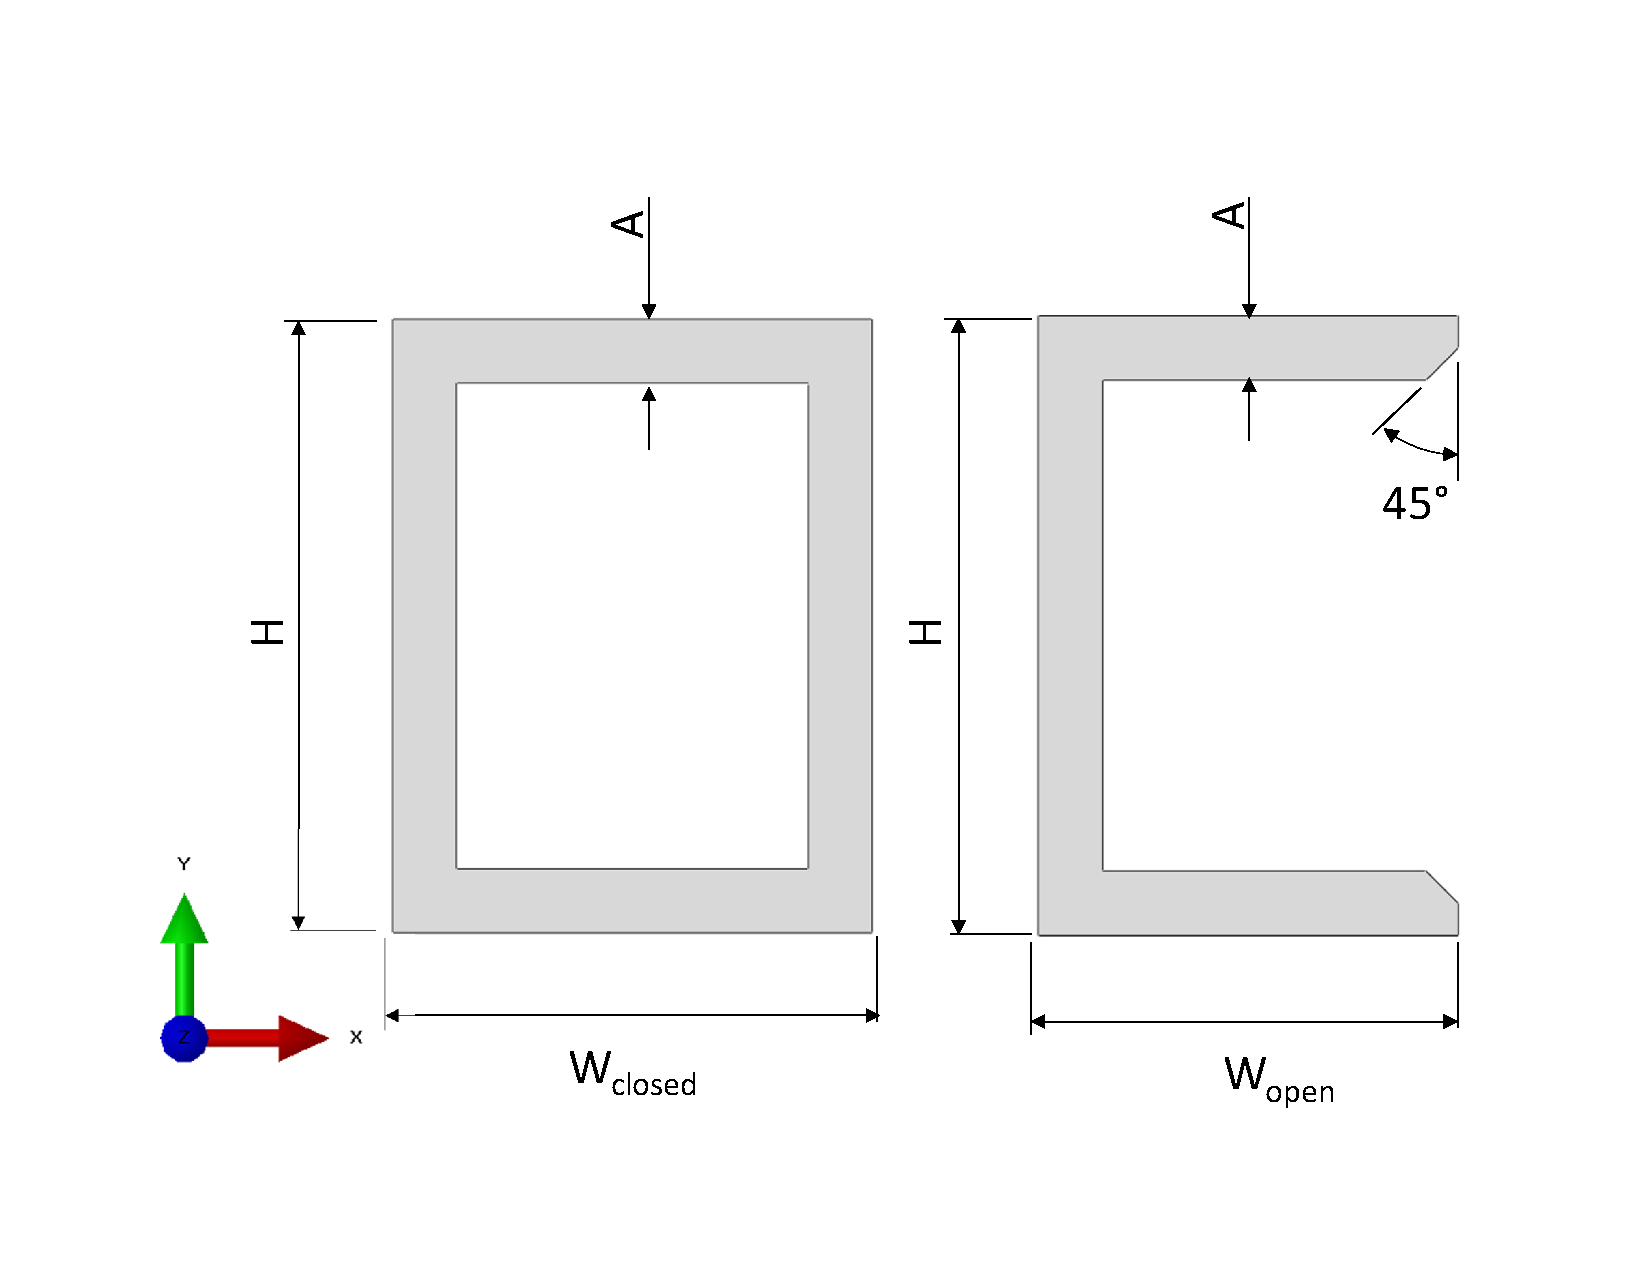
\includegraphics[width=0.8 \textwidth]{model/rib-internalParameters}
      \caption[Internal parameters of the two different ribs parts]{Internal parameters of the two different ribs parts.}\label{fig:rib-internalParameters}
    \end{figure}

    Therefore, the only tailorable parameters for the ribs configurations are the thickness $t_{\mathrm{rib}}$ and the frame width $A_{\mathrm{rib}}$. The nominal value and units of these two parameters together with the nominal value and units of the remaining dependent parameters can be read in Table \ref{tab:parameters_rib}. The Young's modulus was increase one order of magnitude in comparison of that of the wing-box in order to ensure no out-of-plane deformation of the rib.

    \begin{table}[!htpb]
    \centering
    \begin{tabular}{|l|lll|}
    \hline
    \textbf{Parameter} & \multicolumn{1}{l|}{\textbf{Symbol}} & \multicolumn{1}{l|}{\textbf{Units}} & \textbf{Nominal value} \\ \hline \hline
    {\textbf{Dimensions}} &  &  &  \\ \hline
    Rib height & \multicolumn{1}{l|}{$H_{\mathrm{rib}}$} & \multicolumn{1}{l|}{mm} & 383.27 \\ \hline
    Closed rib width & \multicolumn{1}{l|}{$W_{\mathrm{rib,close}}$} & \multicolumn{1}{l|}{mm} & 300 \\ \hline
    Frame width & \multicolumn{1}{l|}{$A_{\mathrm{rib}}$} & \multicolumn{1}{l|}{mm} & 30 \\ \hline
    Rib thickness & \multicolumn{1}{l|}{$t_{\mathrm{rib}}$} & \multicolumn{1}{l|}{mm} & 2 \\ \hline \hline
    {\textbf{Material (Aluminum, 10xE)}} &  &  &  \\ \hline
    Young's modulus & \multicolumn{1}{l|}{$E_{\mathrm{rib}}$} & \multicolumn{1}{l|}{N/mm$^2$} & 690000 \\ \hline
    Poisson's ratio & \multicolumn{1}{l|}{$\nu_{\mathrm{rib}}$} & \multicolumn{1}{l|}{} & 0.3269 \\ \hline
    \end{tabular}
    \caption[Parameters used for the ribs model]{Parameters used for the ribs model. The Young's modulus was increase one order of magnitude in comparison of that of the wing-box in order to ensure no out-of-plane deformation of the rib. The value of the rib width $W_{\mathrm{rib,close}}$ and the height $H_{\mathrm{rib}}$ will be equal to the wing-box width $W_{\mathrm{box}}$ and to the chiral lattice structure height, respectively.}
    \label{tab:parameters_rib}
    \end{table}

  \clearpage
  \subsection{Model mesh} \label{subsec:mesh_computationalModel}

    In the present section, the mesh used in the model will be presented. The mesh was unstructured and it was auto-generated by Abaqus CAE for the whole assembly. The elements were a combination of quadratic and tetrahedral with 4 and 3 nodes, respectively. Different mesh elements size were assigned to different parts of the model depending of the stress complexity expected.

    In Figure \ref{fig:mesh}, it is possible to distinguish two regions that were assigned with different mesh size: the lattice structure and near region of the wing-box skin was assigned with a fine mesh size while the remaining model was assigned with a course mesh, typically one order of magnitude greater. This introduces two new parameters that are used to modify the mesh size of the different regions:

    \begin{itemize}
      \item $S_{\mathrm{f}}$: Fine mesh size
      \item $S_{\mathrm{c}}$: Course mesh size
    \end{itemize}

    \begin{figure}[!htpb]
      \centering
      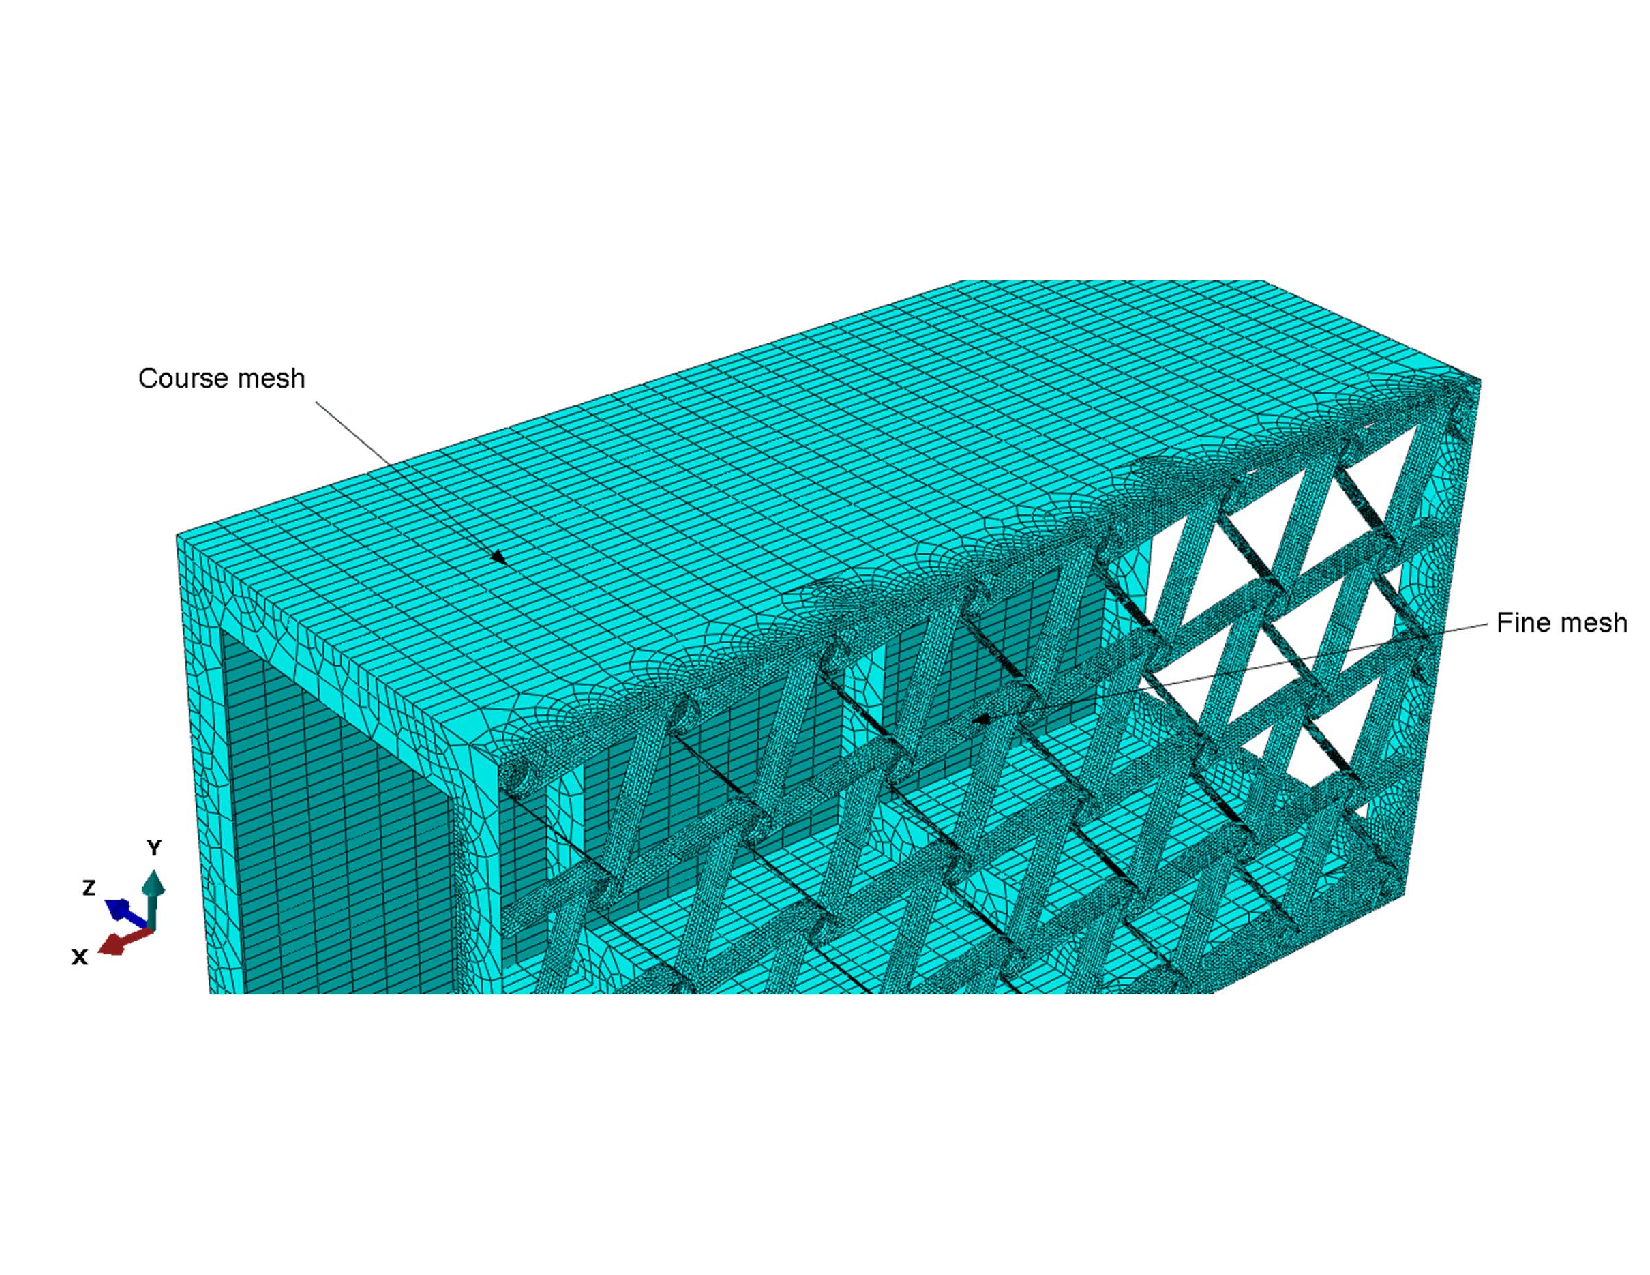
\includegraphics[width=0.8 \textwidth]{model/mesh}
      \caption[Internal parameters of the two different ribs parts]{Internal parameters of the two different ribs parts. Different mesh elements size were assigned to different parts of the model. The lattice structure was assigned with a fine mesh element size while the wing-box was assigned with a course mesh element size.}\label{fig:mesh}
    \end{figure}

  \clearpage
  \subsection{Attachment points modeling} \label{subsec:connections_computationalModel}

    %General thoughts:
    % - Necessity of applying condition node to node
    %
    %Equation contrainsts issues:
    % - Slow down simulations
    %
    %Coupling constrainsts:
    %
    %
    In the present subsection, the FEM modeling of the connection between the lattice nodes and the wing box is presented. This is an unavoidable transition from the lattice structure of nodes and ligaments to the skin of the wing box. Loads are transmitted to the lattice through this attachment points that is why its design results crucial.

    There will be three different configurations that were studied:

    \begin{description}
      \item[Blocked translation and rotation] The lattice nodes have all its degrees of freedom restrained
      \item[Blocked translation and free rotation] The lattice nodes are free to rotate around its own axis but the translation the direction parallel to the skin is restrained. An sketch showing this connection can be viewed in Figure \ref{fig:connectionModeling1}. This configuration was the one chosen for the demonstrator built in the Figure \ref{fig:connectionLatticeNodesToSkin}.
      \item[Free translation and rotation] Now the lattice nodes is allowed to translate parallel to the skin. This configuration is schematically represented in Figure \ref{fig:connectionModeling2}.
    \end{description}

    \begin{figure}[!htpb]
      \centering
      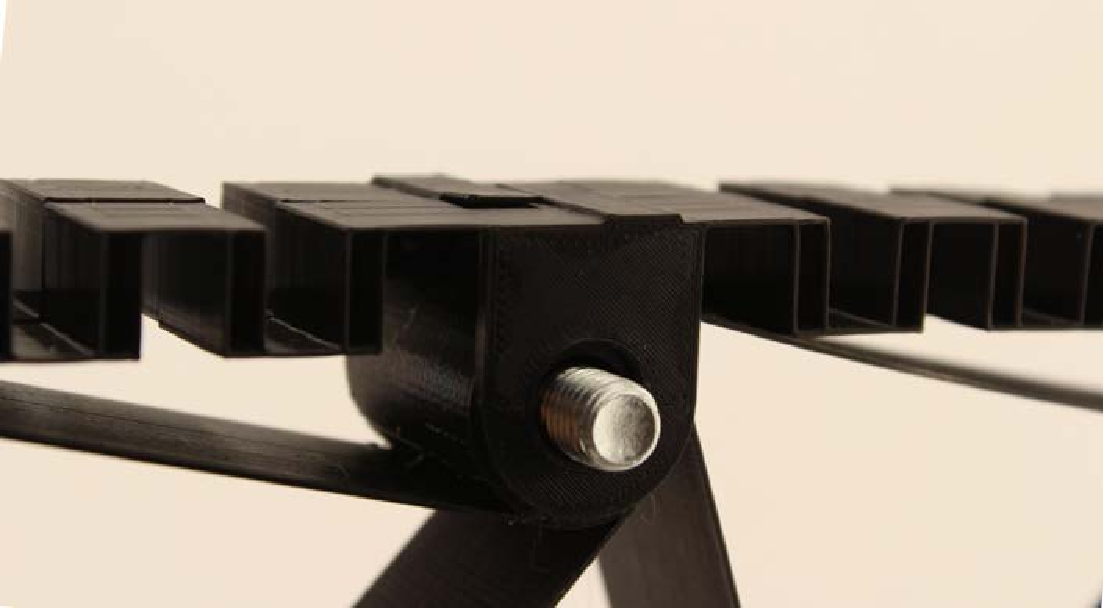
\includegraphics[width=0.8 \textwidth]{model/connectionLatticeNodesToSkin}
      \caption[Detail of the connection between the lattice nodes and the skin]{Detail of the connection between the lattice nodes and the skin. The picture shows the type of connection chosen for the manufactured demonstrator of the lattice. The lattice nodes is allowed to rotate around its own axis but cannot translate parallel to the skin. \cite{Vincenz2017}}\label{fig:connectionLatticeNodesToSkin}
    \end{figure}

    \begin{figure}[!htpb]
      \centering
      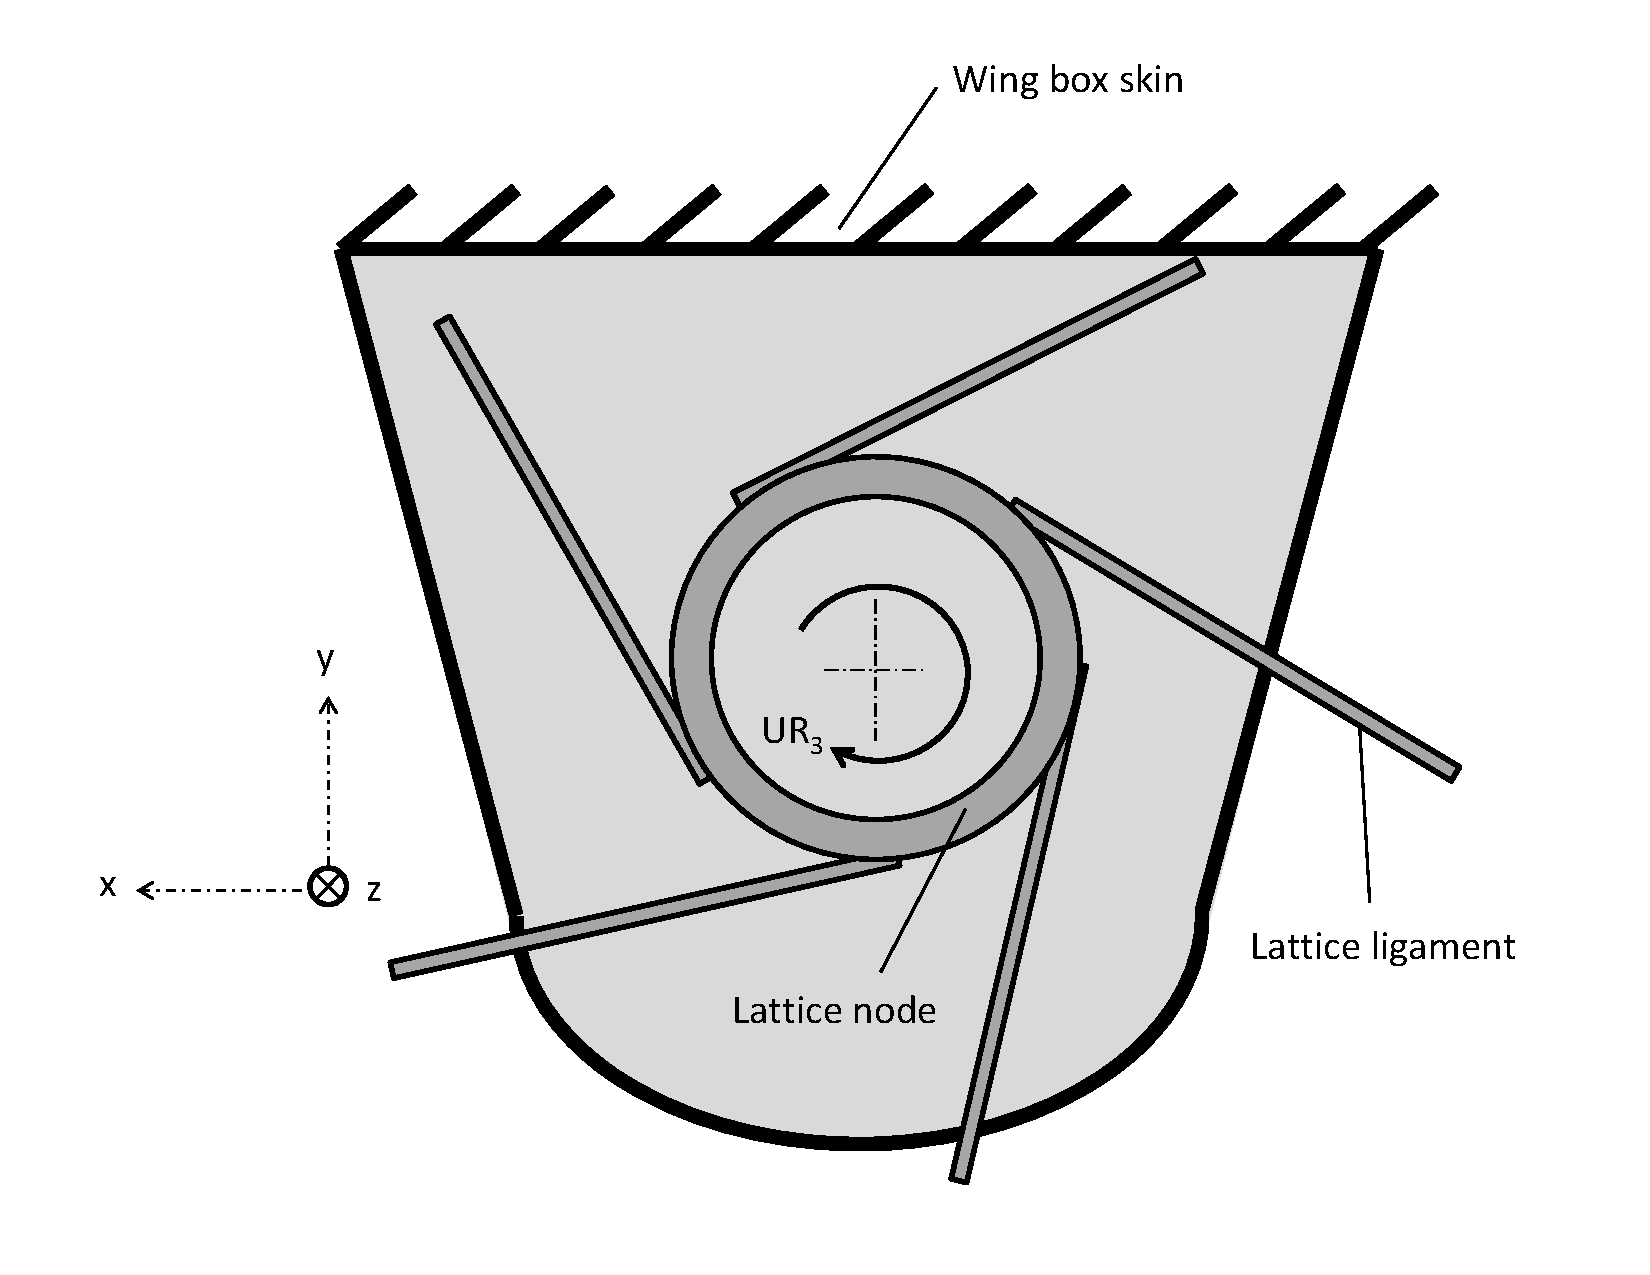
\includegraphics[width=0.8 \textwidth]{model/connectionModeling1}
      \caption[Blocked translation and free rotation connection between the lattice nodes and the skin]{Blocked translation and free rotation connection between the lattice nodes and the skin. In this case, the only degree of freedom of the lattice node that it is not restrained the rotation around its own axis, that is the rotation $UR_3$ around the direction $z$.}\label{fig:connectionModeling1}
    \end{figure}

    \begin{figure}[!htpb]
      \centering
      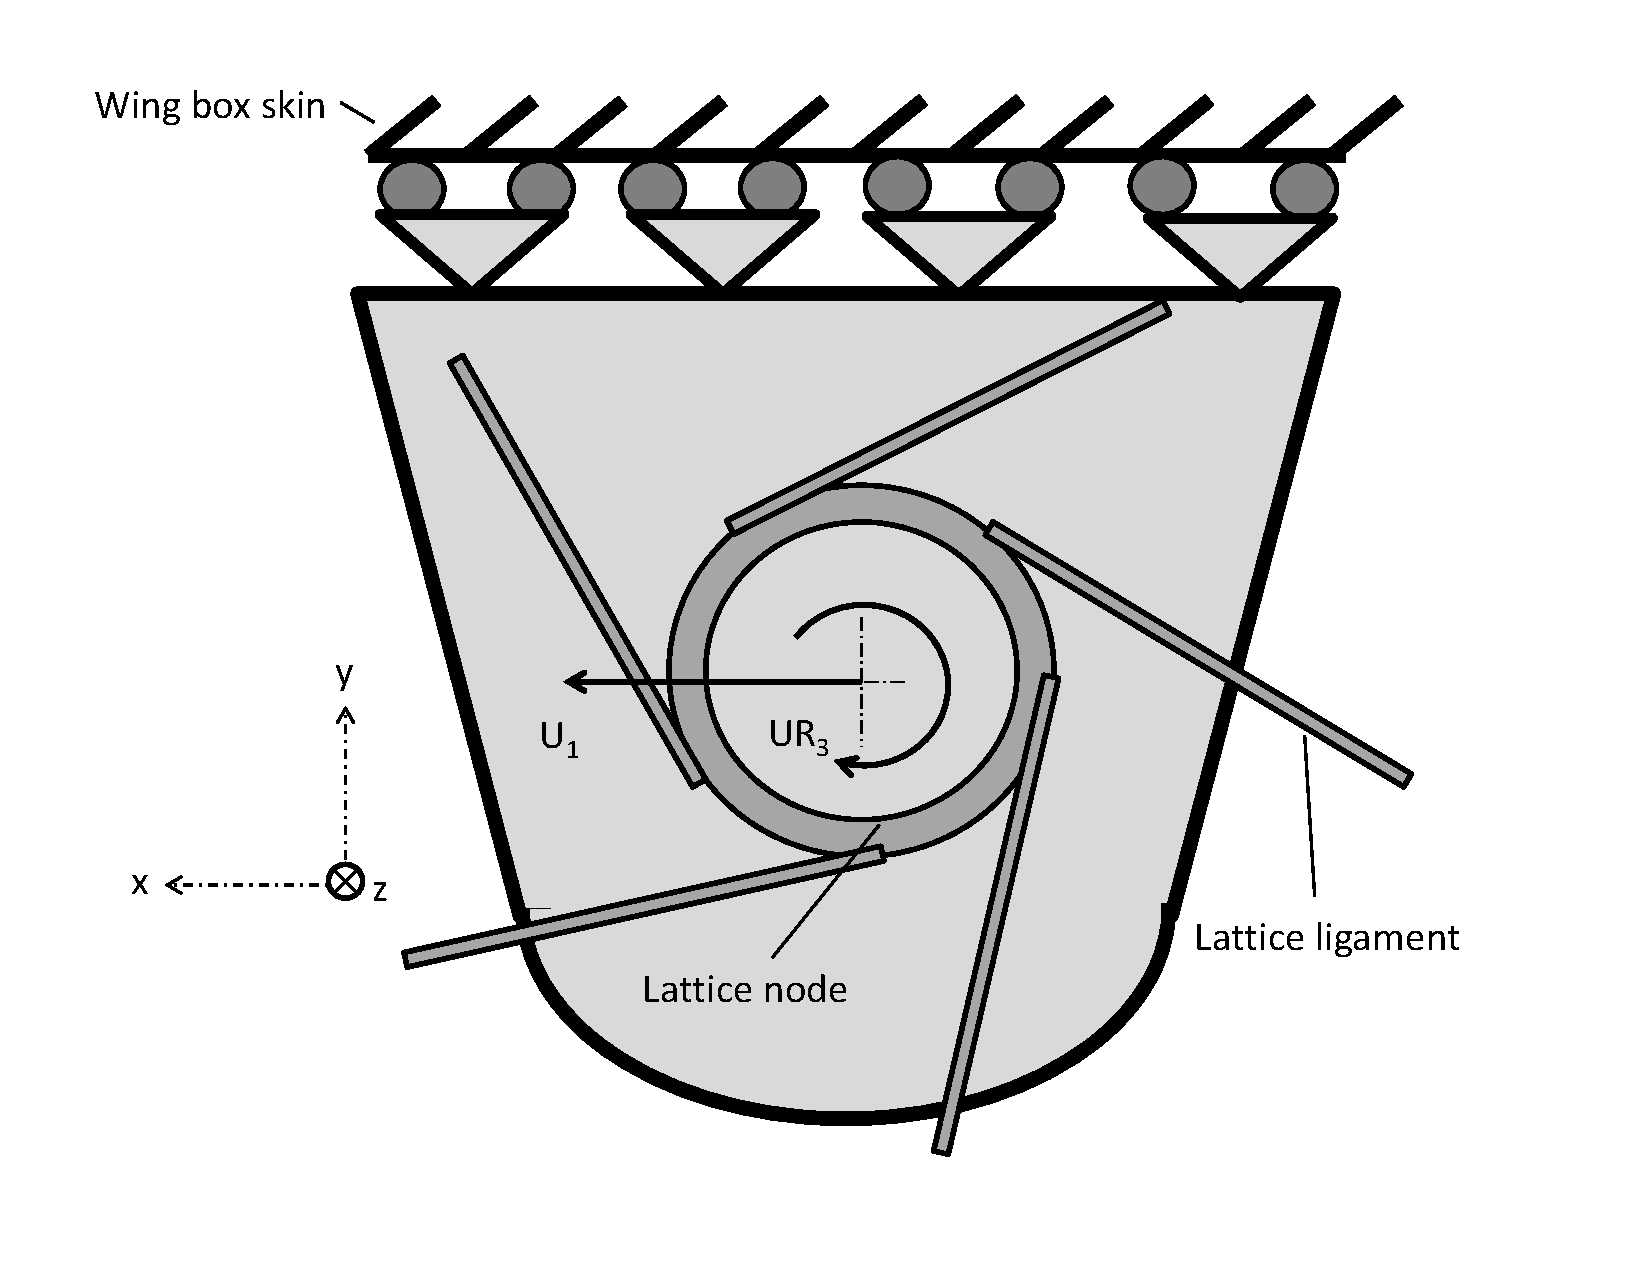
\includegraphics[width=0.8 \textwidth]{model/connectionModeling2}
      \caption[Free translation and rotation connection between the lattice nodes and the skin]{Free translation and rotation connection between the lattice nodes and the skin. For this case, the unrestrained degrees of freedom of the lattice nodes are the rotation the rotation $UR_3$ around its own axis, i.e.: the direction $z$; and the displacement $U_1$ parallel to the wing-box wall, i.e.: along the direction $x$.}\label{fig:connectionModeling2}
    \end{figure}

    In the FEM model, the three connections where modeled using different approaches. Since the lattice of chiral elements and the skin of the wing box were not physical connected by any element, it was necessary to use of the interaction modules provided by Abaqus CAE. There a different options available to constrain the degrees of freedom of a particular set of mesh nodes to another set of mesh nodes. Some of these modules were already explored in Subsection \ref{subsec:parametrization_Model} when investigating how to model the lattice nodes rigid body behavior.

    \subsubsection{Coupling through tyre part}

    This approach consisted in using the tyre part that was described in Subsection \ref{subsec:parametrization_Model}. In each of the lattice nodes located at the border of the lattice structure, a tyre part was created and embed into the lattice node, as it was shown in Figure \ref{fig:tyre-connection}. Then, a coupling constraint is establish between a mesh node in the middle of the tyre and a mesh node located on the wing-box skin just above the tyre, as shown in Figure \ref{fig:connection-tyre}.

    \begin{figure}[!htpb]
      \centering
      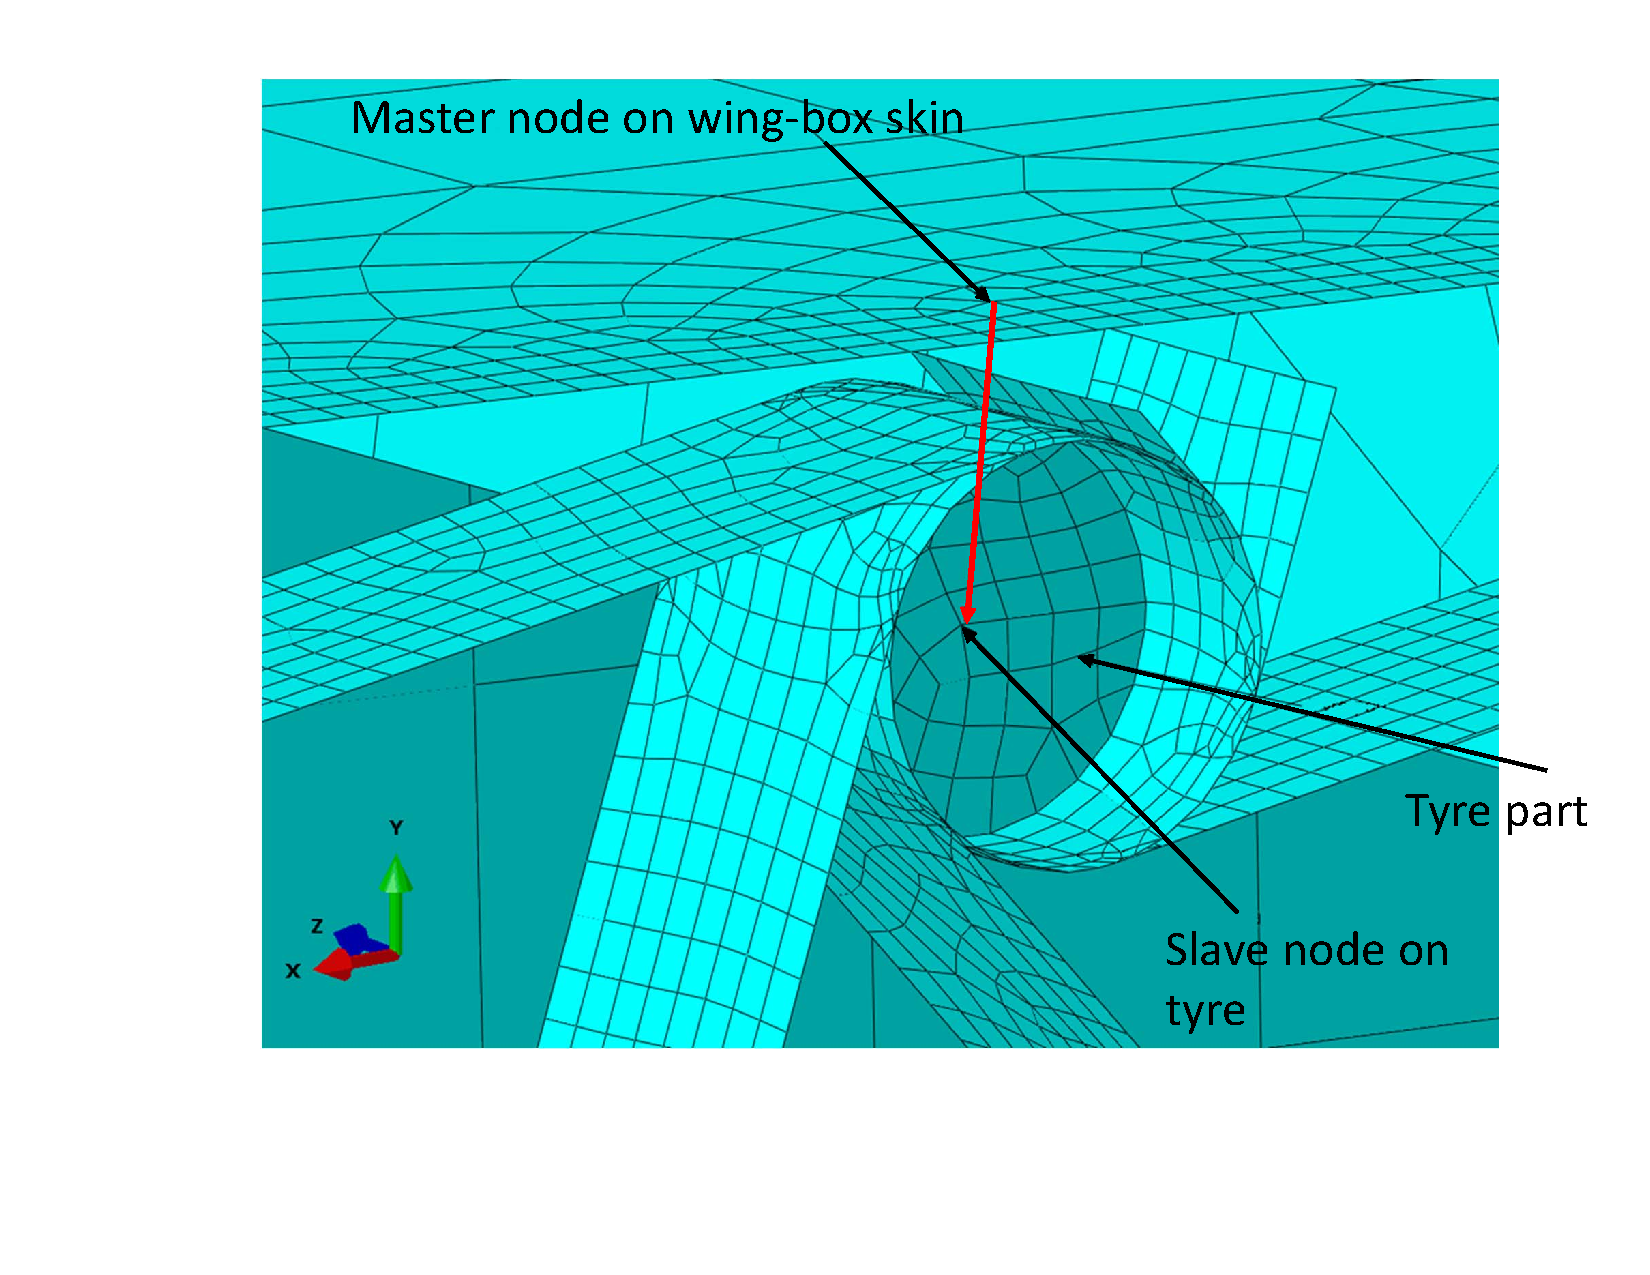
\includegraphics[width=0.8 \textwidth]{model/connection-tyre}
      \caption[Coupling condition between the lattice node and the wing-box skin through tyre]{Coupling condition between the lattice node and the wing-box skin through tyre. The coupling condition is establish between a mesh node located in the wing-box skin that acts as a master node and a mesh node in the middle of the tyre that becomes the coupling node.}\label{fig:connection-tyre}
    \end{figure}

    Depending on the type of connection considered, there will be different degrees of freedom the ones that are coupled. For the most restrictive case, in which the connection between the lattice structure and the wing-box is rigid, not allowing any displacement, the six degrees of freedom will be coupled between the mesh nodes mentioned on the previous paragraph.

    For the other connection types, rotation of the lattice node is allowed around its own axis. This allowance is implemented by not constraining the rotation $UR_3$ around the $z$ direction in the coupling constraint definition. Finally, the last connection type explained at the beginning of the present subsection allowed the displacement of the lattice node parallel to the wing-box skin. For this case, the translation $U_1$ along the $x$ direction is be left uncoupled.

    The rigid body motion imposed to the mesh node located at the center of the tyre is translated to the mesh nodes located in the faces of the lattice node because they are physically connected.

    \subsubsection{Coupling through local cylindrical reference system}

    In this case, the rigid body characteristic provided by the tyre installation is substituted by an additional coupling condition that is establish in a local cylindrical reference system located at each of the lattice nodes. This new reference system substitutes the global Cartesian coordinates system and its origin is a reference point located in the centre of the lattice node,  at $z=B/2$mm. The position of a point in the lattice node face will be determined by the radial distance $r$ to the origin, the angular position $\theta$ and the position $z$ along the node rotation axis. An sketch of this reference system is shown in Figure \ref{fig:connection-localSYS1}. In order to ensure the

    In the mentioned local reference system, a kinematic coupling constrain link the rigid body motion of the radial position $r$ and the position $z$ of a reference point to those of a set of mesh nodes located on the lattice node faces. In the coupling definition, the reference point is the master node and the mesh nodes found in the faces of the lattice node are the slave nodes. This condition is visualized in Abaqus as shown in Figure \ref{fig:connection-localSYS2}.

    Then, an additional coupling constrain is necessary to be establish in between the reference node that acts as the origin of the local cylindrical reference system and the wing-box skin. This is the same one that was previously establish when using a tyre part and shown in Figure \ref{fig:connection-tyre}. The only difference is that for this case the slave node is the reference point instead of a mesh node located in the center of the tyre.

    \begin{figure}[!htpb]
      \centering
      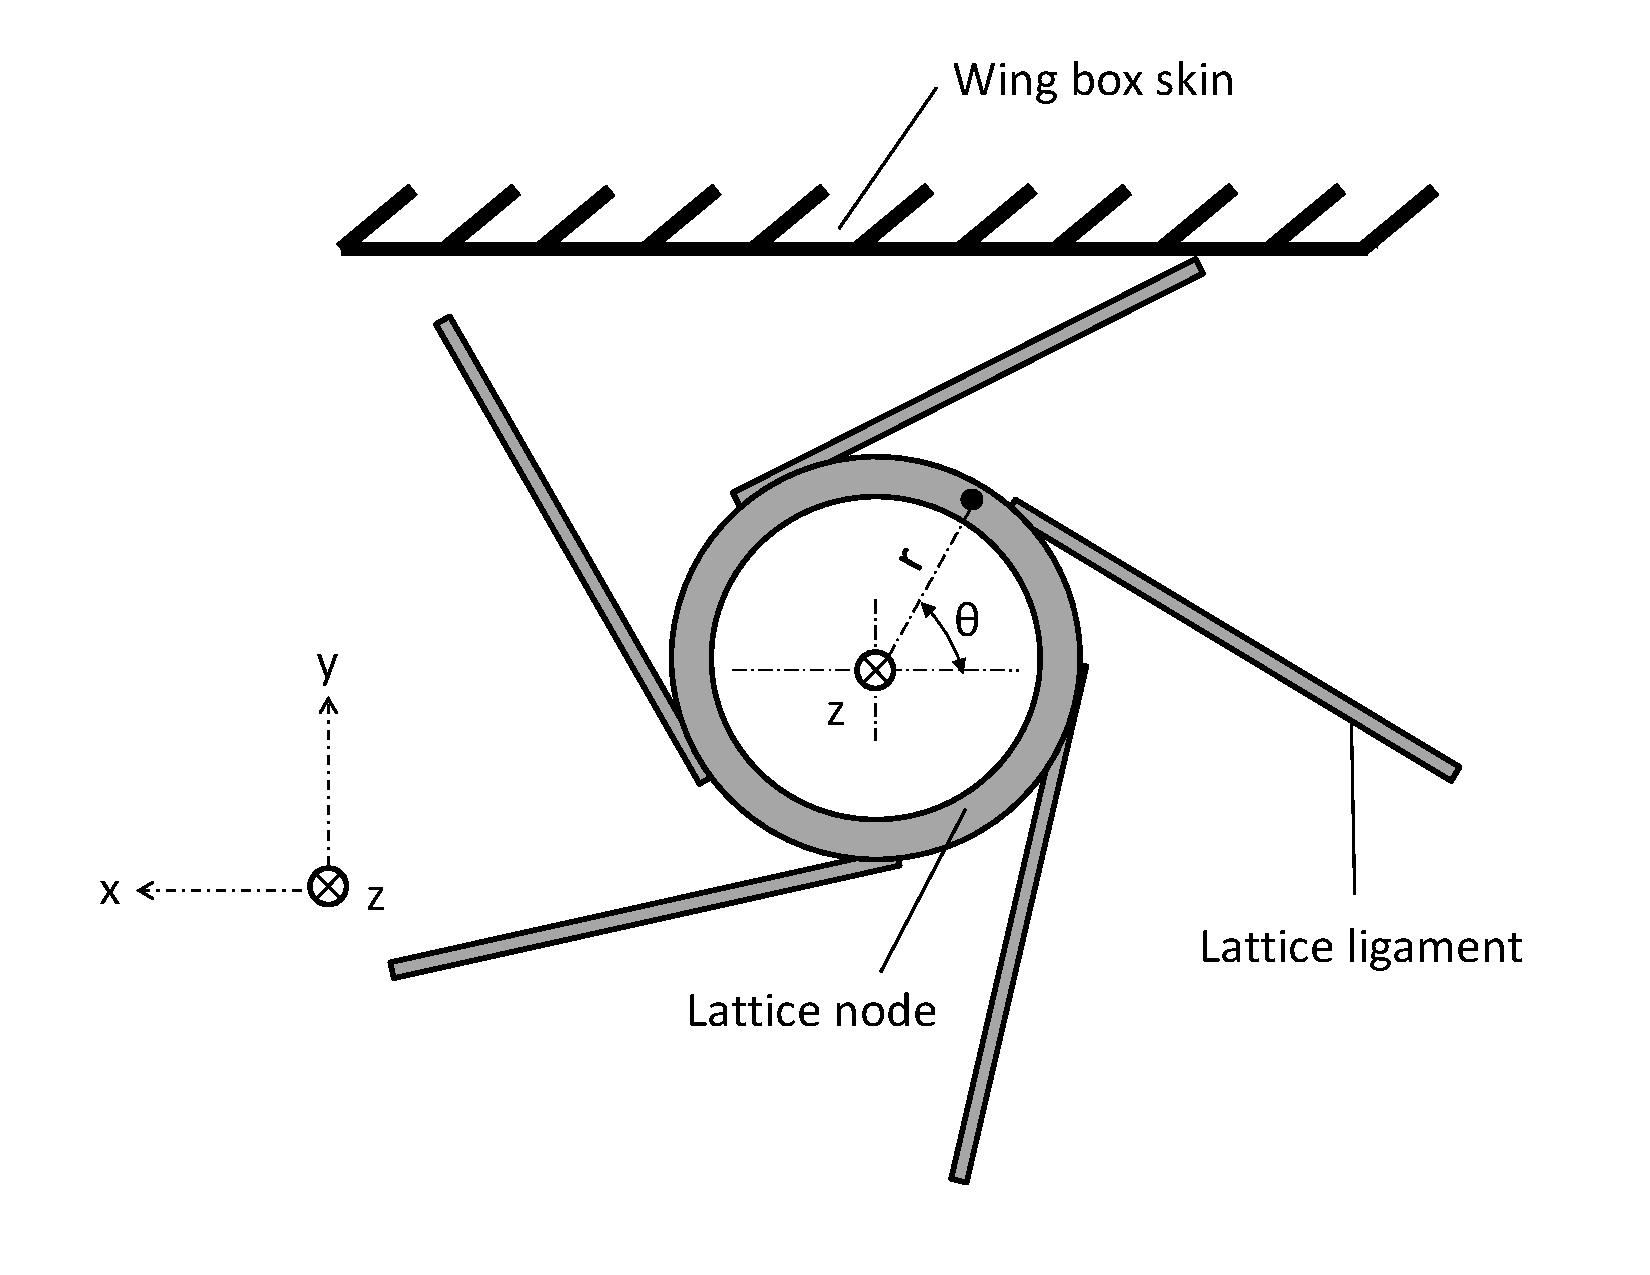
\includegraphics[width=0.8 \textwidth]{model/connection-SYS1}
      \caption[Local reference system at the lattice nodes]{Local reference system at the lattice nodes. The position of point in the lattice node faces will be determined by the radial distance $r$ to the origin, the angular position $\theta$ and the position $z$ along the node rotation axis.}\label{fig:connection-localSYS1}
    \end{figure}

    \begin{figure}[!htpb]
      \centering
      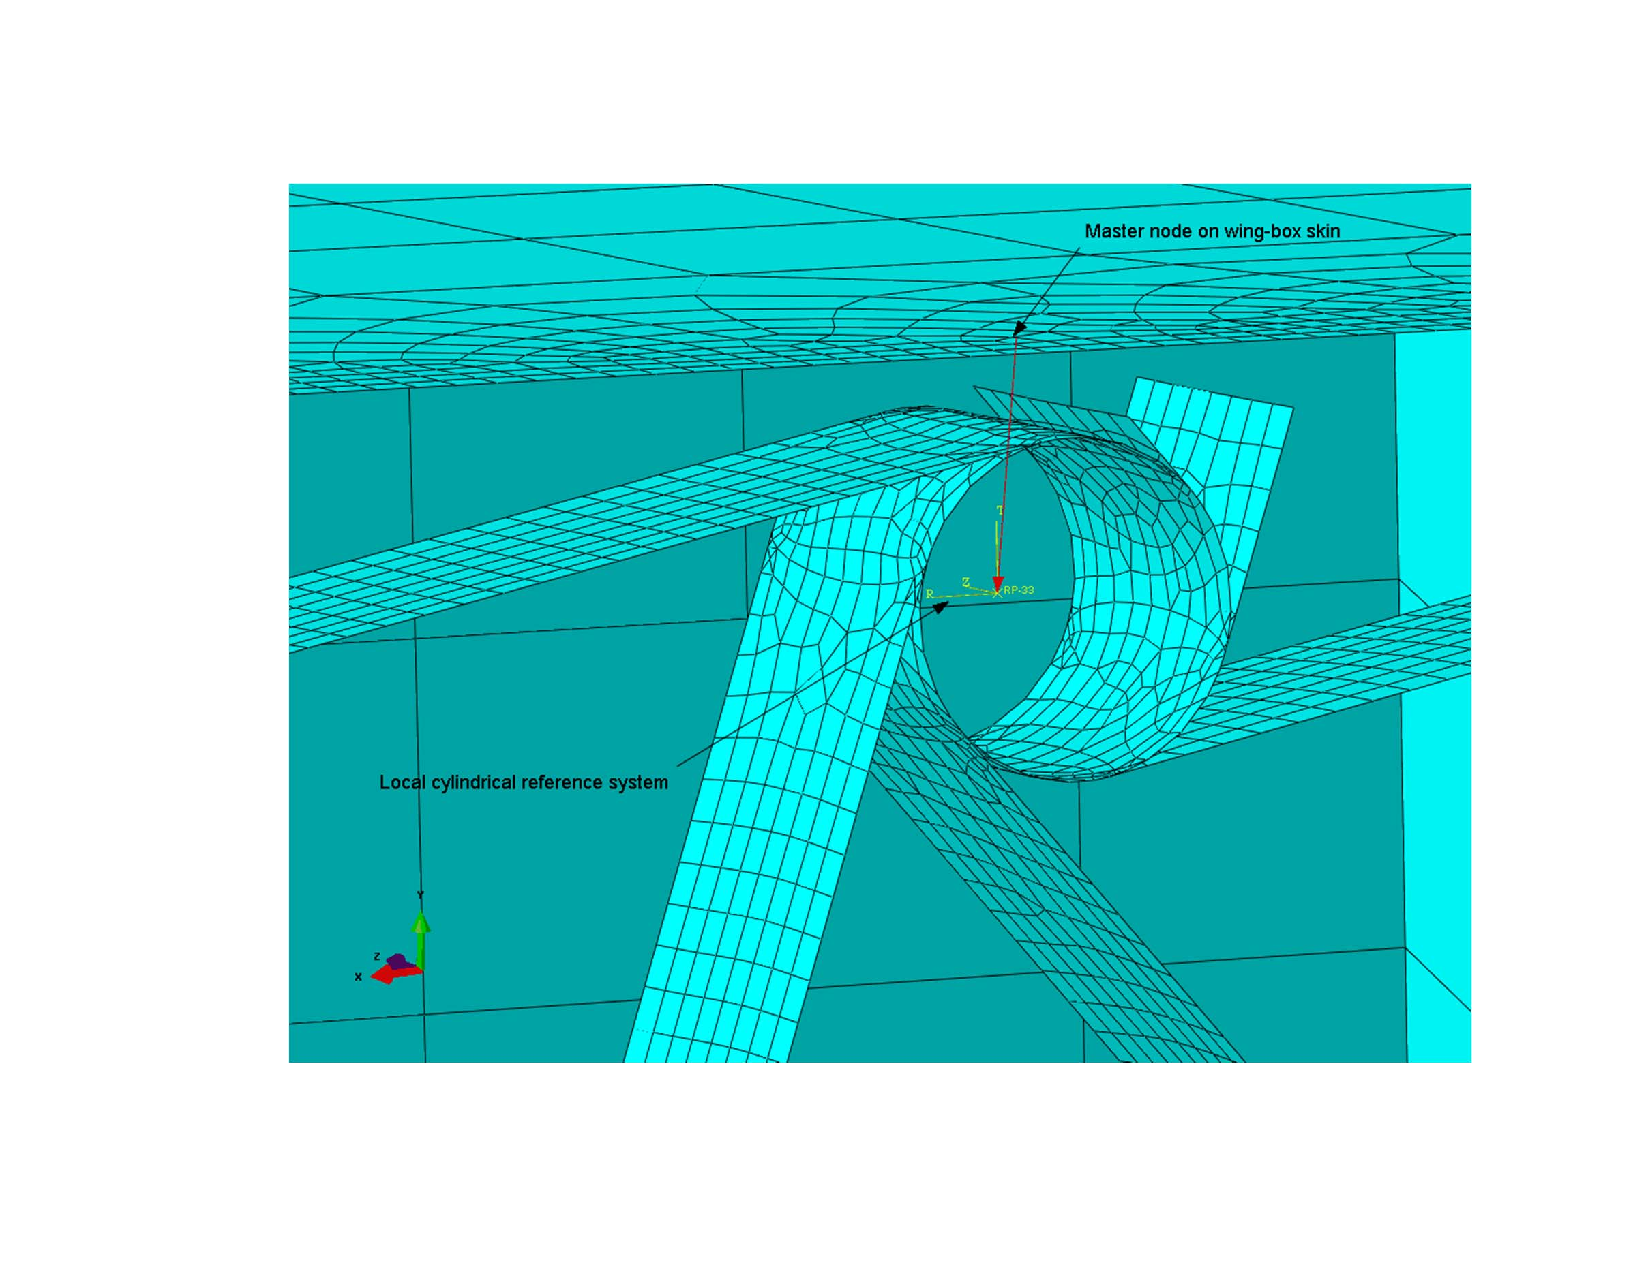
\includegraphics[width=0.8 \textwidth]{model/connection-SYS2}
      \caption[Coupling condition between the lattice node and the wing-box skin through a local reference system]{Coupling condition between the lattice node and the wing-box skin through a local reference system. }\label{fig:connection-localSYS2}
    \end{figure}

  \clearpage
  \subsection{Parametric study method} \label{subsec:parametricStudy_computationalModel}

    The model was described in the previous subsections was implemented in a Python program that was read by the FEM software, Abaqus. This enables the possibility of executing different simulations for different values of the parameters introduced previously. An schematic characterization of the program execution is shown the flow chart represented in Figure \ref{fig:flowChart}.

    \begin{figure}[!htpb]
      \centering
      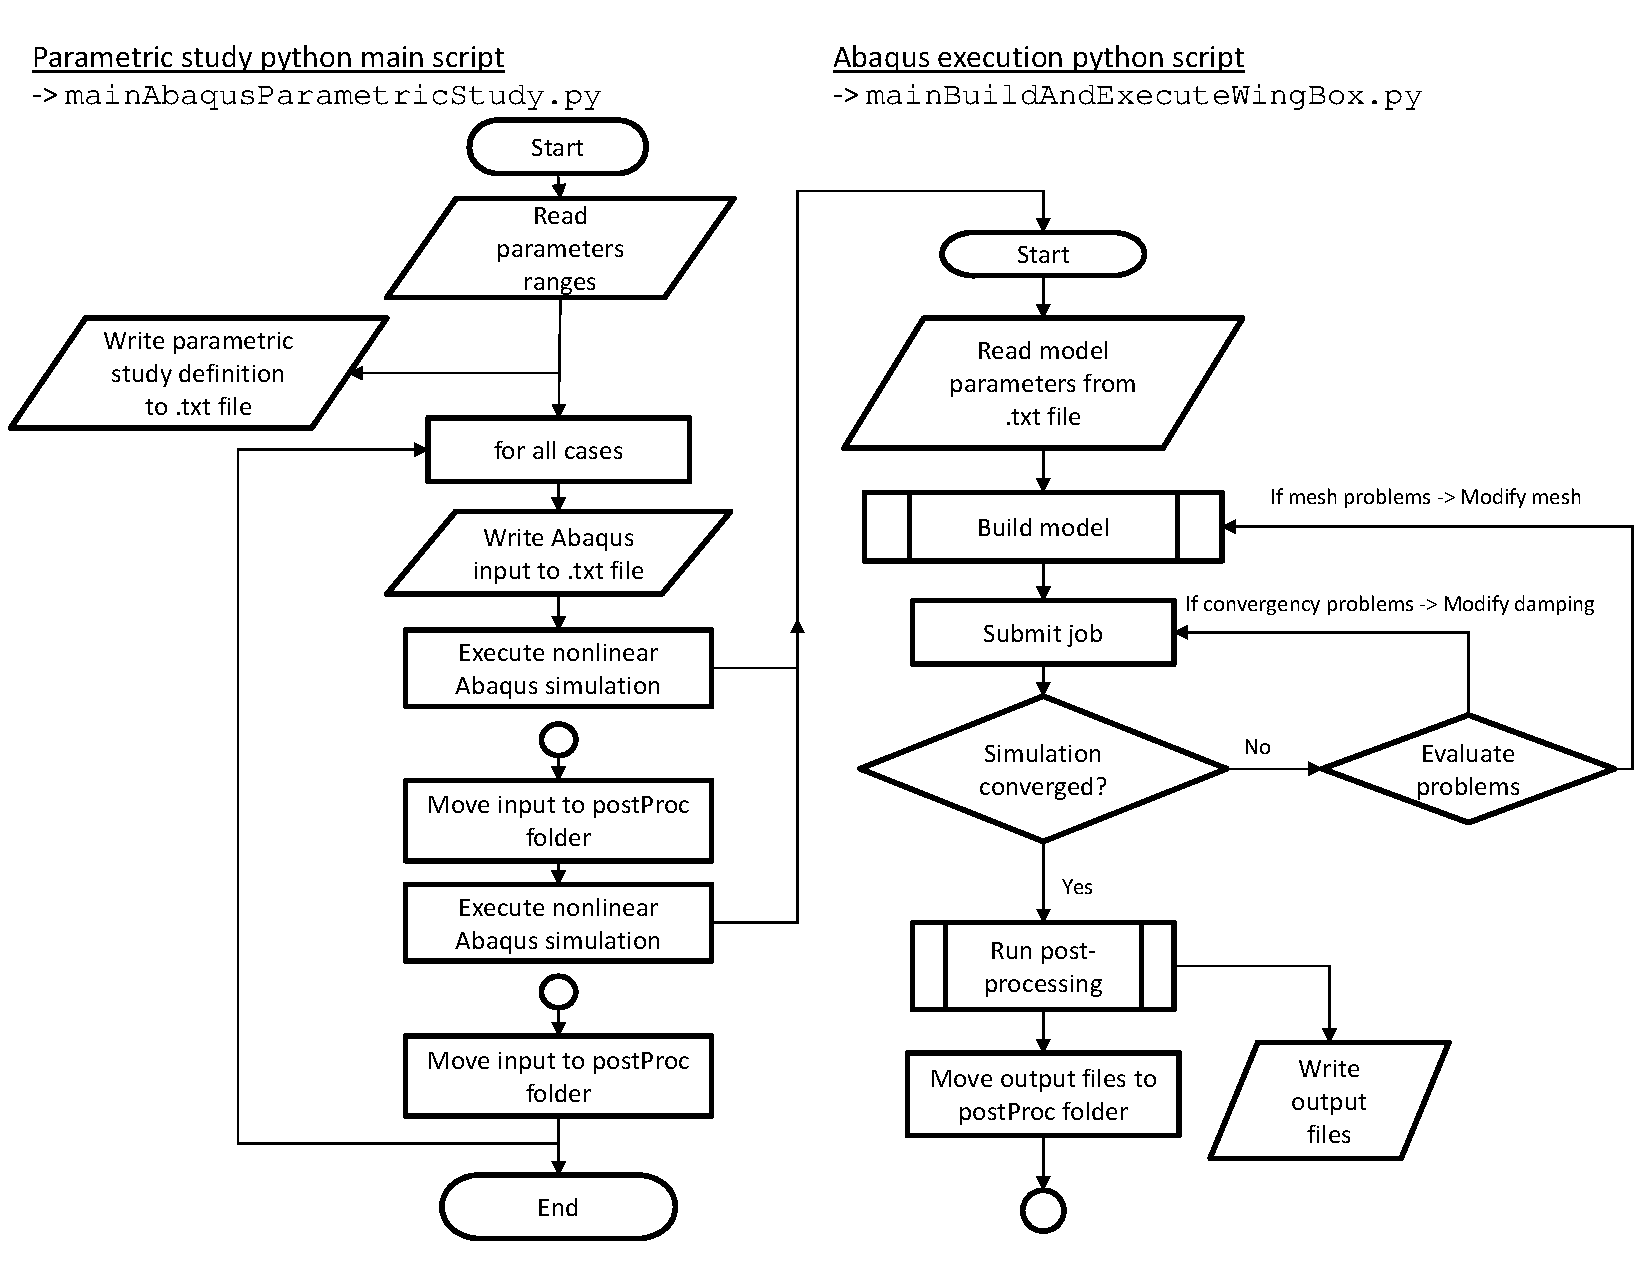
\includegraphics[width=0.8 \textwidth]{model/flowChart}
      \caption[Flow chart showing the execution of the parametric study code]{Flow chart showing the execution of the parametric study code. }\label{fig:flowChart}
    \end{figure}

\ClearDoublePageOrNot{\controlClearPage}
\chapter{Results} \label{chap:Results}

\section{Introduction} \label{sec:intro_Results}

% Introduction to the chapter

\subsection{Parametric study on the analytical model} \label{subsec:parametricStudy_Results} 
In the present subsection, the variation of the beam properties for different parameter values will be shown. The beam geometry will be characterized through the cross-sectional aspect ratio $B/H$, the thickness ratio $t_2/t_1$ and the slenderness ratio $L/B$. The effect of these parameters on the sectional properties, twist and bending stiffness, and flexural and twisting compliance will be shown. Additionally, the variance of the stiffness ratio $E_1/E_2$ will also be included in the analysis.

\subsubsection{Results} \label{subsubsec:results_parametricStudy}

The influence of the cross-sectional aspect ratio $B/H$ on the torsional stiffness $G I_t$, the shear centre position $y_{\mathrm{SC}}$ and the flexural stiffness $E I_y$ is shown in Figures \ref{fig:GIt-E1overE2-BoverH}, \ref{fig:SC-E1overE2-BoverH} and \ref{fig:EIy-E1overE2-BoverH}, respectively. On its side, the effect of thickness ratio $t_2/t_1$ on the same three beam parameters is shown in Figures \ref{fig:GIt-E1overE2-t2overt1}, \ref{fig:SC-E1overE2-t2overt1} and \ref{fig:EIy-E1overE2-t2overt1}.

Additionally, the effect of the cross-sectional aspect ratio $B/H$ on the deflection and torsional compliance is shown on Figures \ref{fig:woverQ-E1overE2-BoverH} and \ref{fig:phioverQ-E1overE2-BoverH}, respectively. The corresponding plots when analysing the effect of the thickness ratio $t_2/t_1$ on the deflection and torsional compliance are shown on Figures \ref{fig:woverQ-E1overE2-t2overt1} and \ref{fig:phioverQ-E1overE2-t2overt1}, respectively. The beam's torsional compliance will be expressed as fraction of the twist at the tip divided by the vertical force applied, that is $|\phi_{\mathrm{tip}}| / Q$, while the beam deflection compliance will be expressed as fraction of the maximum vertical displacement at the tip divided by the vertical force applied, that is $w_{\mathrm{0,tip}} / Q$.

The effect of the slenderness ratio $L/B$ on the deflection and torsional compliances is shown in Figures \ref{fig:woverQ-E1overE2-LoverB} and \ref{fig:phioverQ-E1overE2-LoverB}, respectively.

%Figures variation of B/H
\begin{figure}[!htpb] %G I_t versus B/H
  \centering
  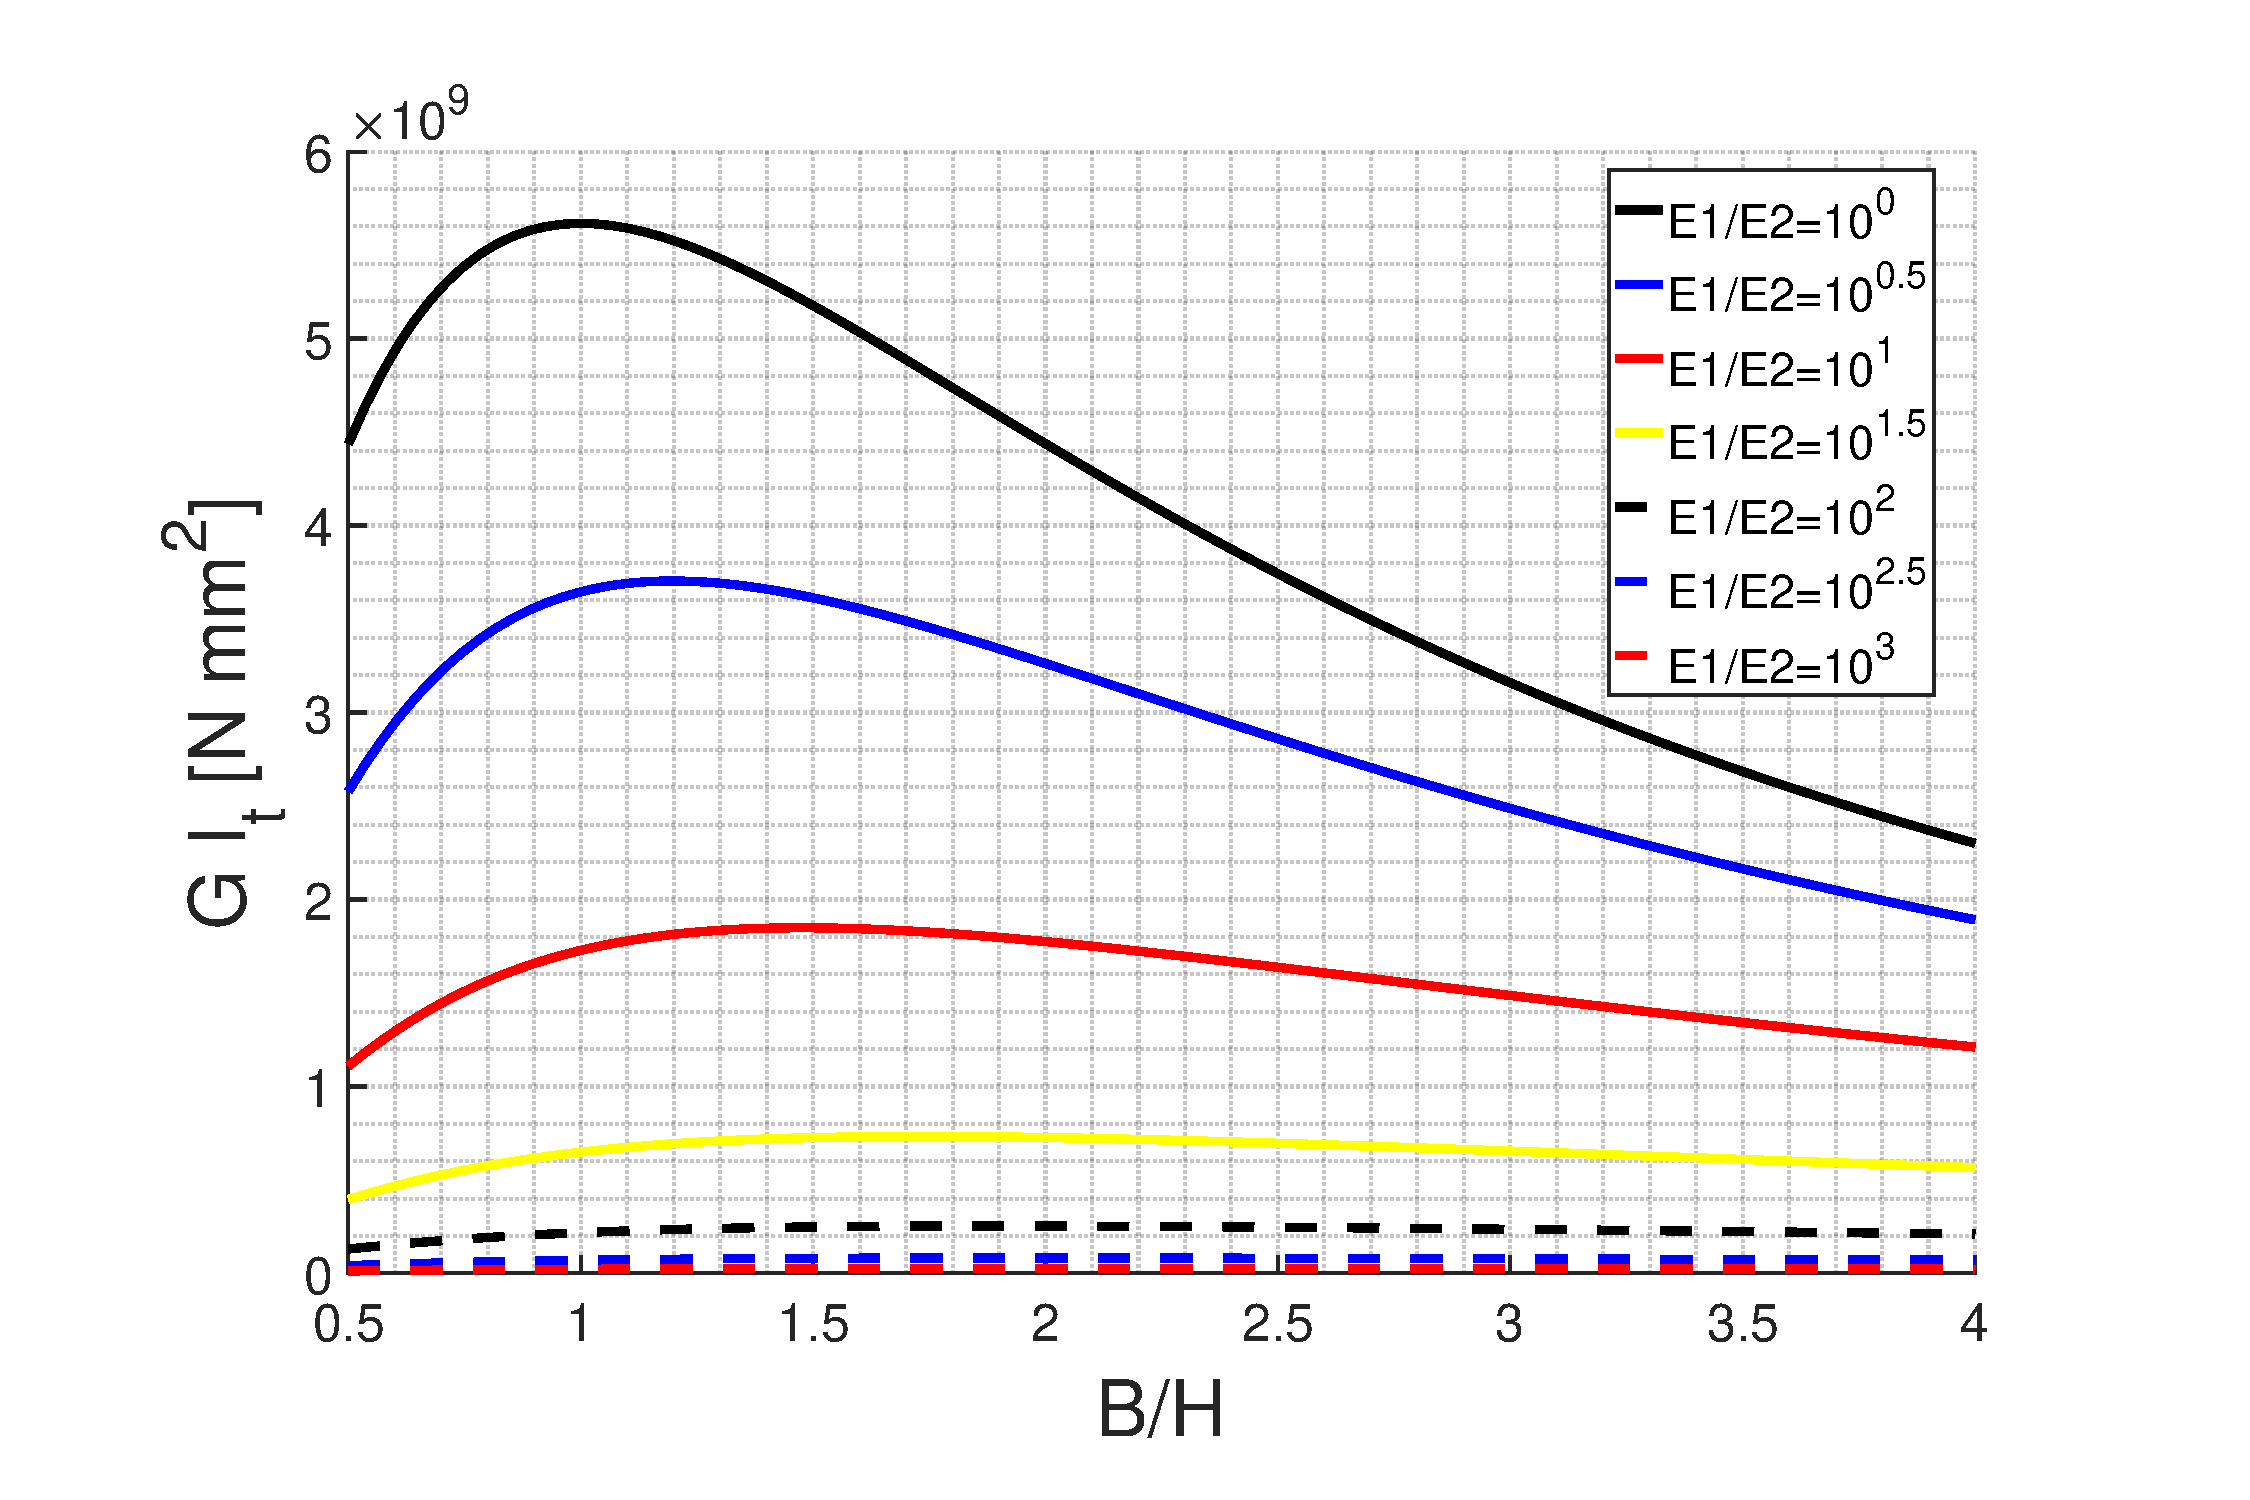
\includegraphics[width=0.8 \textwidth]{../../analytical/figures/GIt-E1overE2-BoverH}
  \caption[Influence of the cross-sectional aspect ratio $B/H$ on the torsional stiffness $GI_t$]{Influence of the cross-sectional aspect ratio $B/H$ on the torsional stiffness $GI_t$ is shown for various values of the stiffness ratio $E_1/E_2$ ranging from $10^0$ to $10^3$. }\label{fig:GIt-E1overE2-BoverH}
\end{figure}

\begin{figure}[!htpb] %Shear centre versus B/H
  \centering
  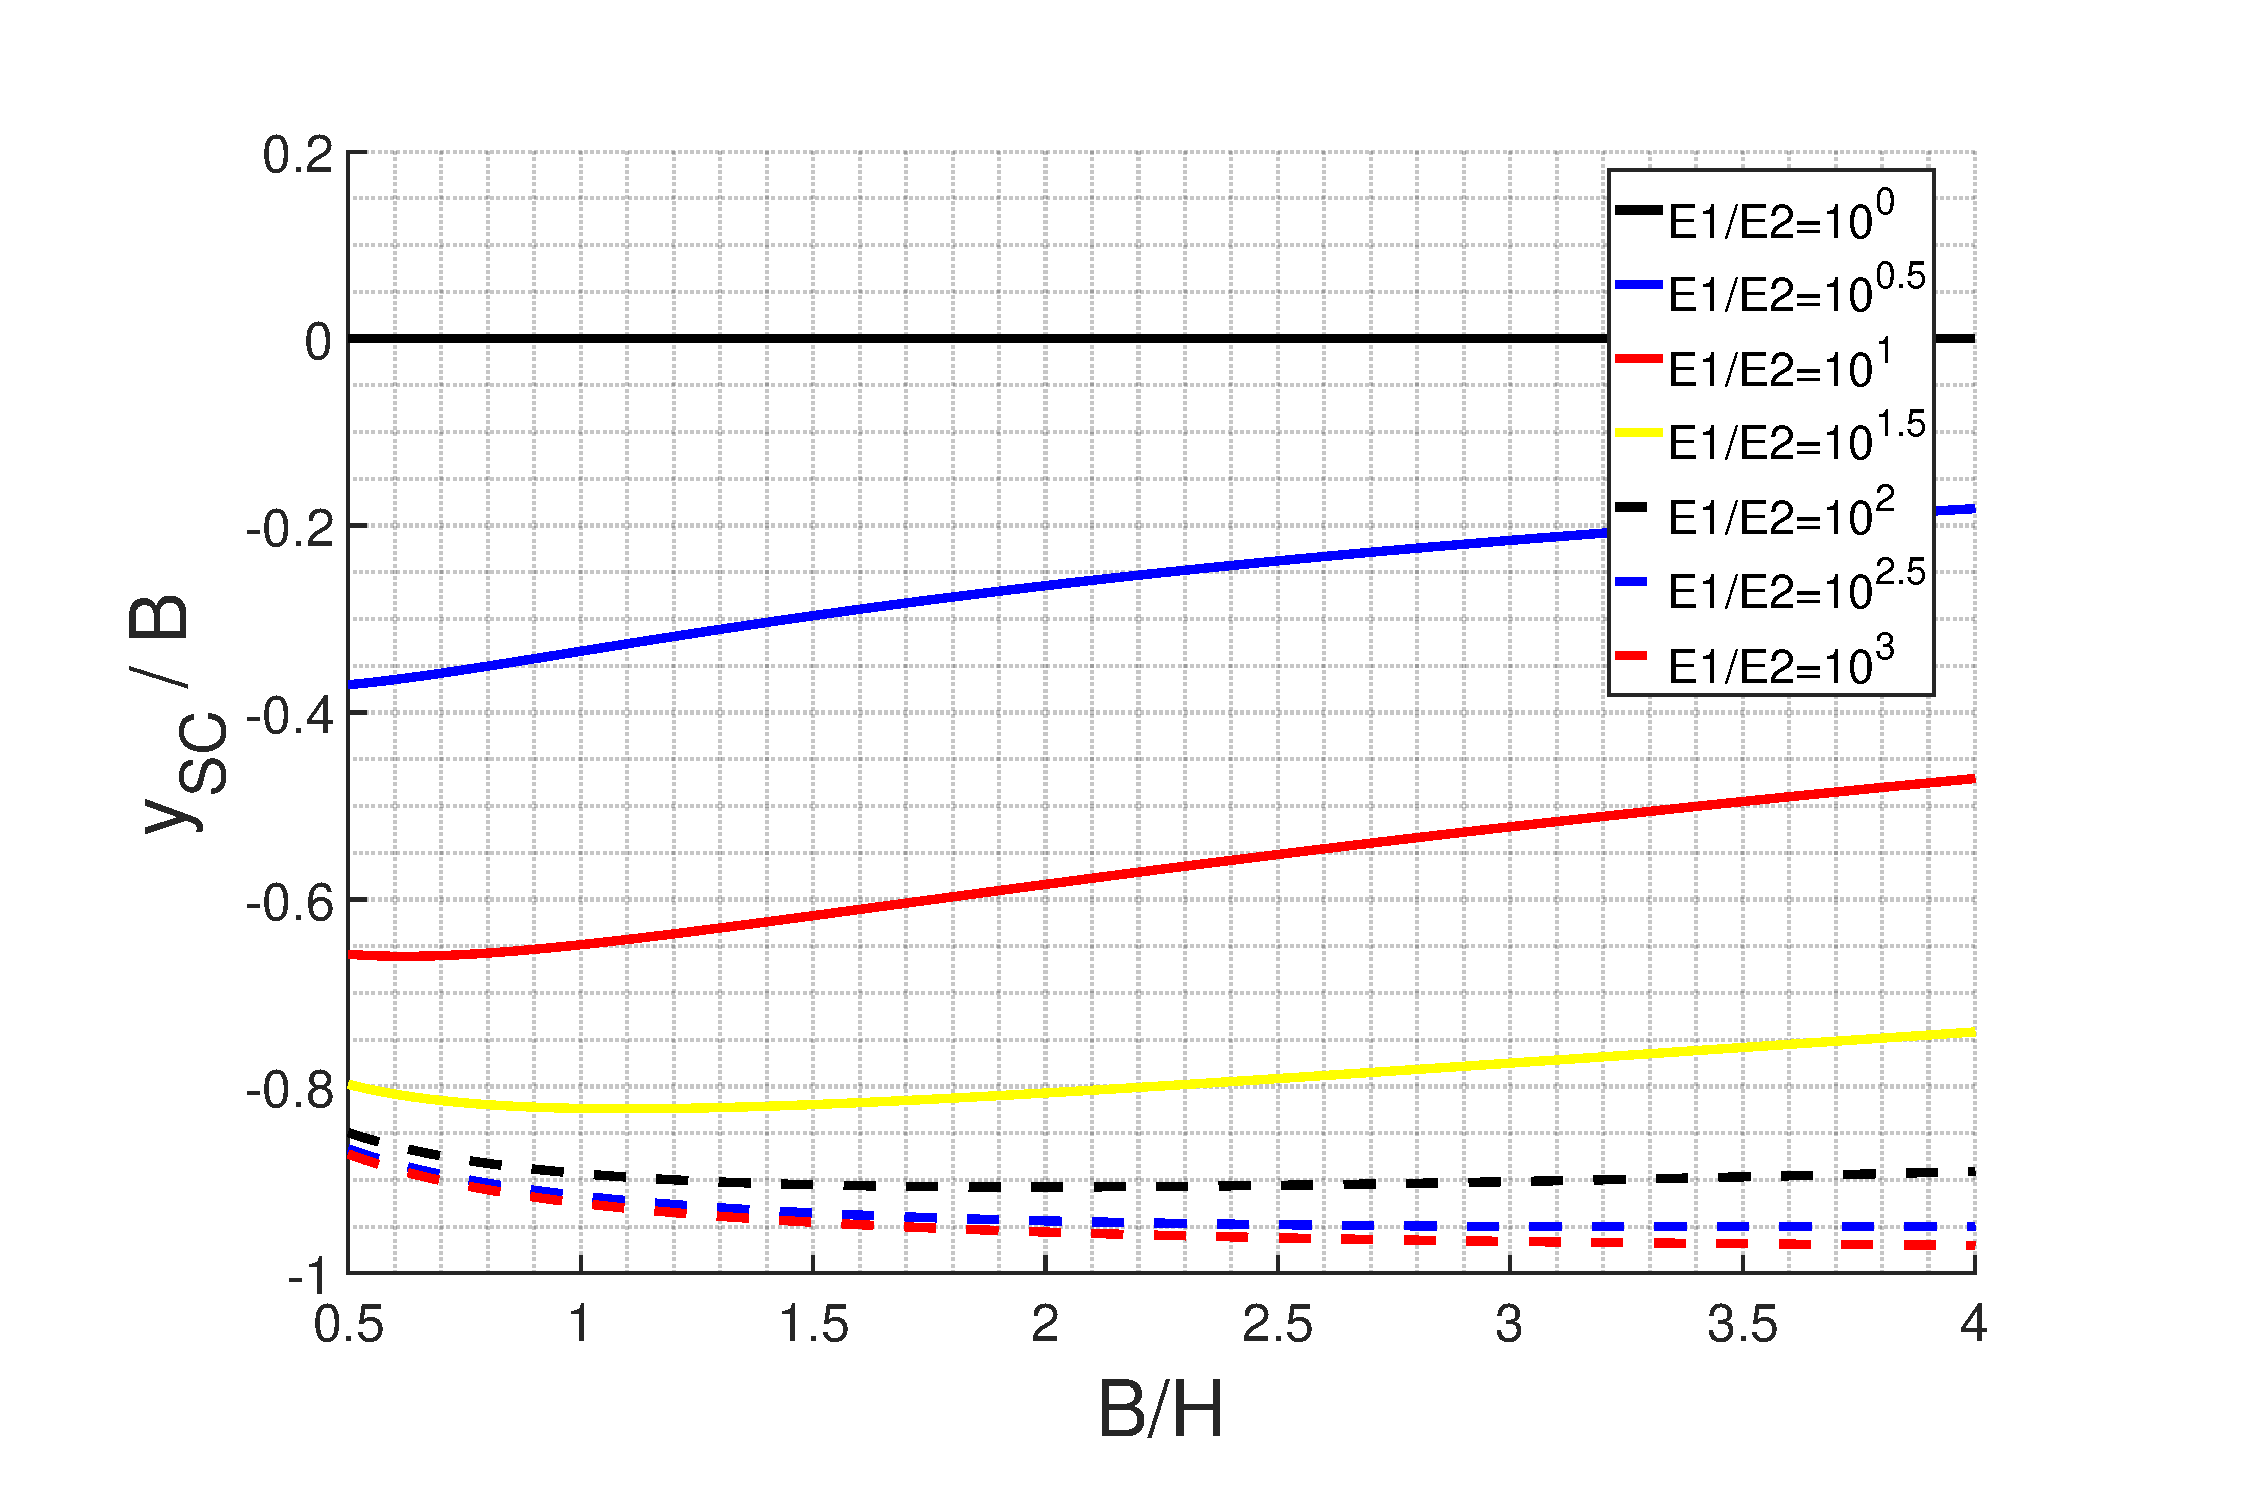
\includegraphics[width=0.8 \textwidth]{../../analytical/figures/SC-E1overE2-BoverH}
  \caption[Influence of the cross-sectional aspect ratio $B/H$ on the dimensionless shear centre position $y_{\mathrm{SC}}/B$]{Influence of the cross-sectional aspect ratio $B/H$ on the dimensionless shear centre position $y_{\mathrm{SC}}/B$ is shown for various values of the stiffness ratio $E_1/E_2$ ranging from $10^0$ to $10^3$. }\label{fig:SC-E1overE2-BoverH}
\end{figure}

\begin{figure}[!htpb] %E I_y = \Phi_y versus B/H
  \centering
  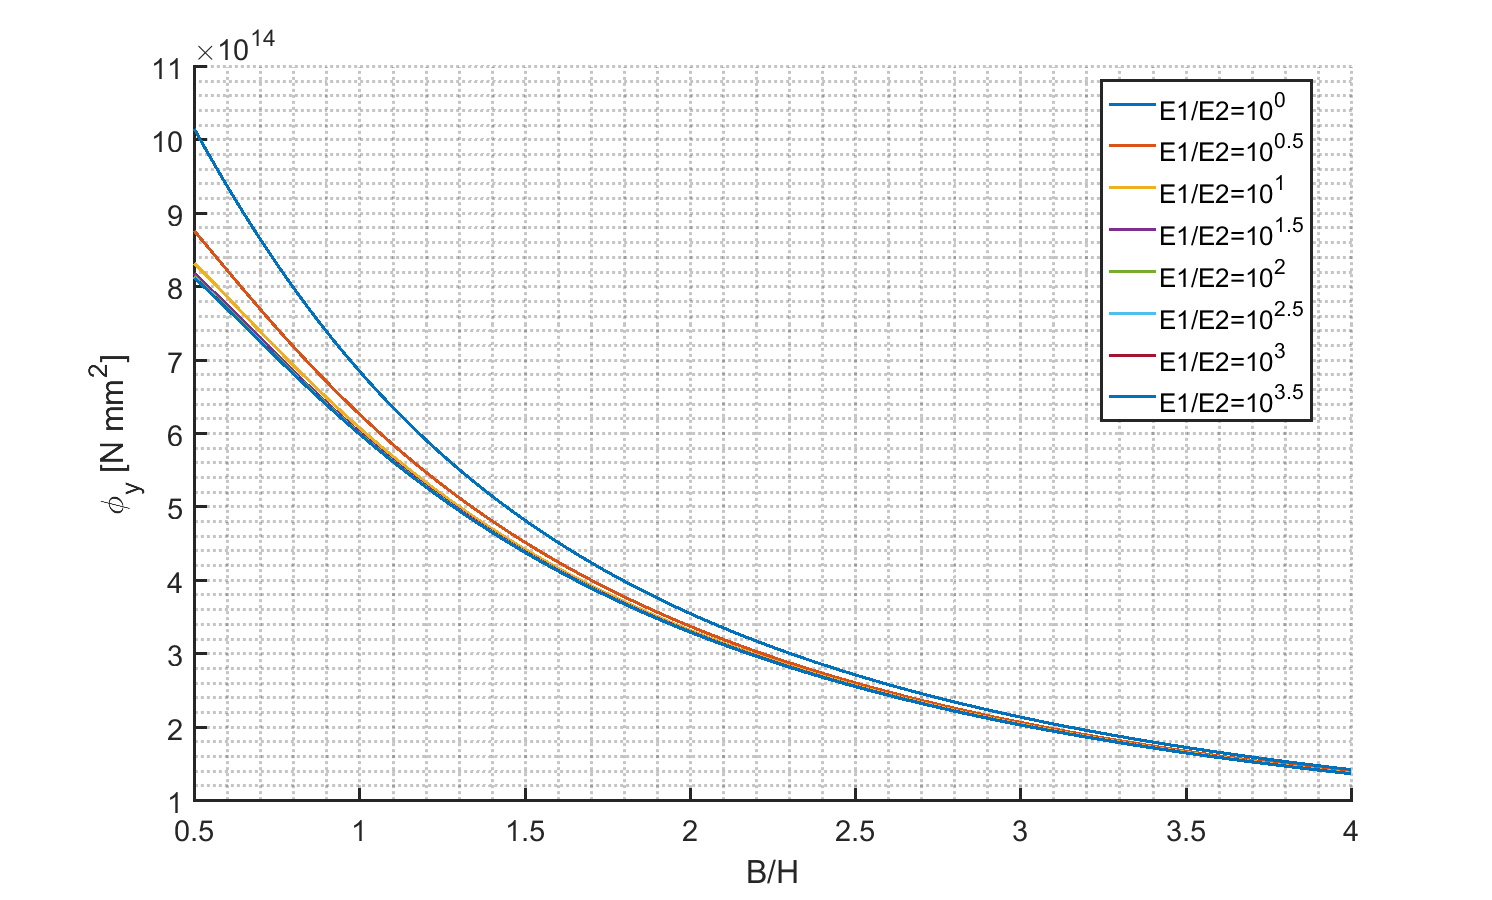
\includegraphics[width=0.8 \textwidth]{../../analytical/figures/EIy-E1overE2-BoverH}
  \caption[Influence of the cross-sectional aspect ratio $B/H$ on the flexural stiffness $EI_y$]{Influence of the cross-sectional aspect ratio $B/H$ on the flexural stiffness $EI_y = \Phi_y$ is shown for various values of the stiffness ratio $E_1/E_2$ ranging from $10^0$ to $10^3$. }\label{fig:EIy-E1overE2-BoverH}
\end{figure}

\begin{figure}[!htpb] %w_0,tip / Q versus B/H, deflection compliance
  \centering
  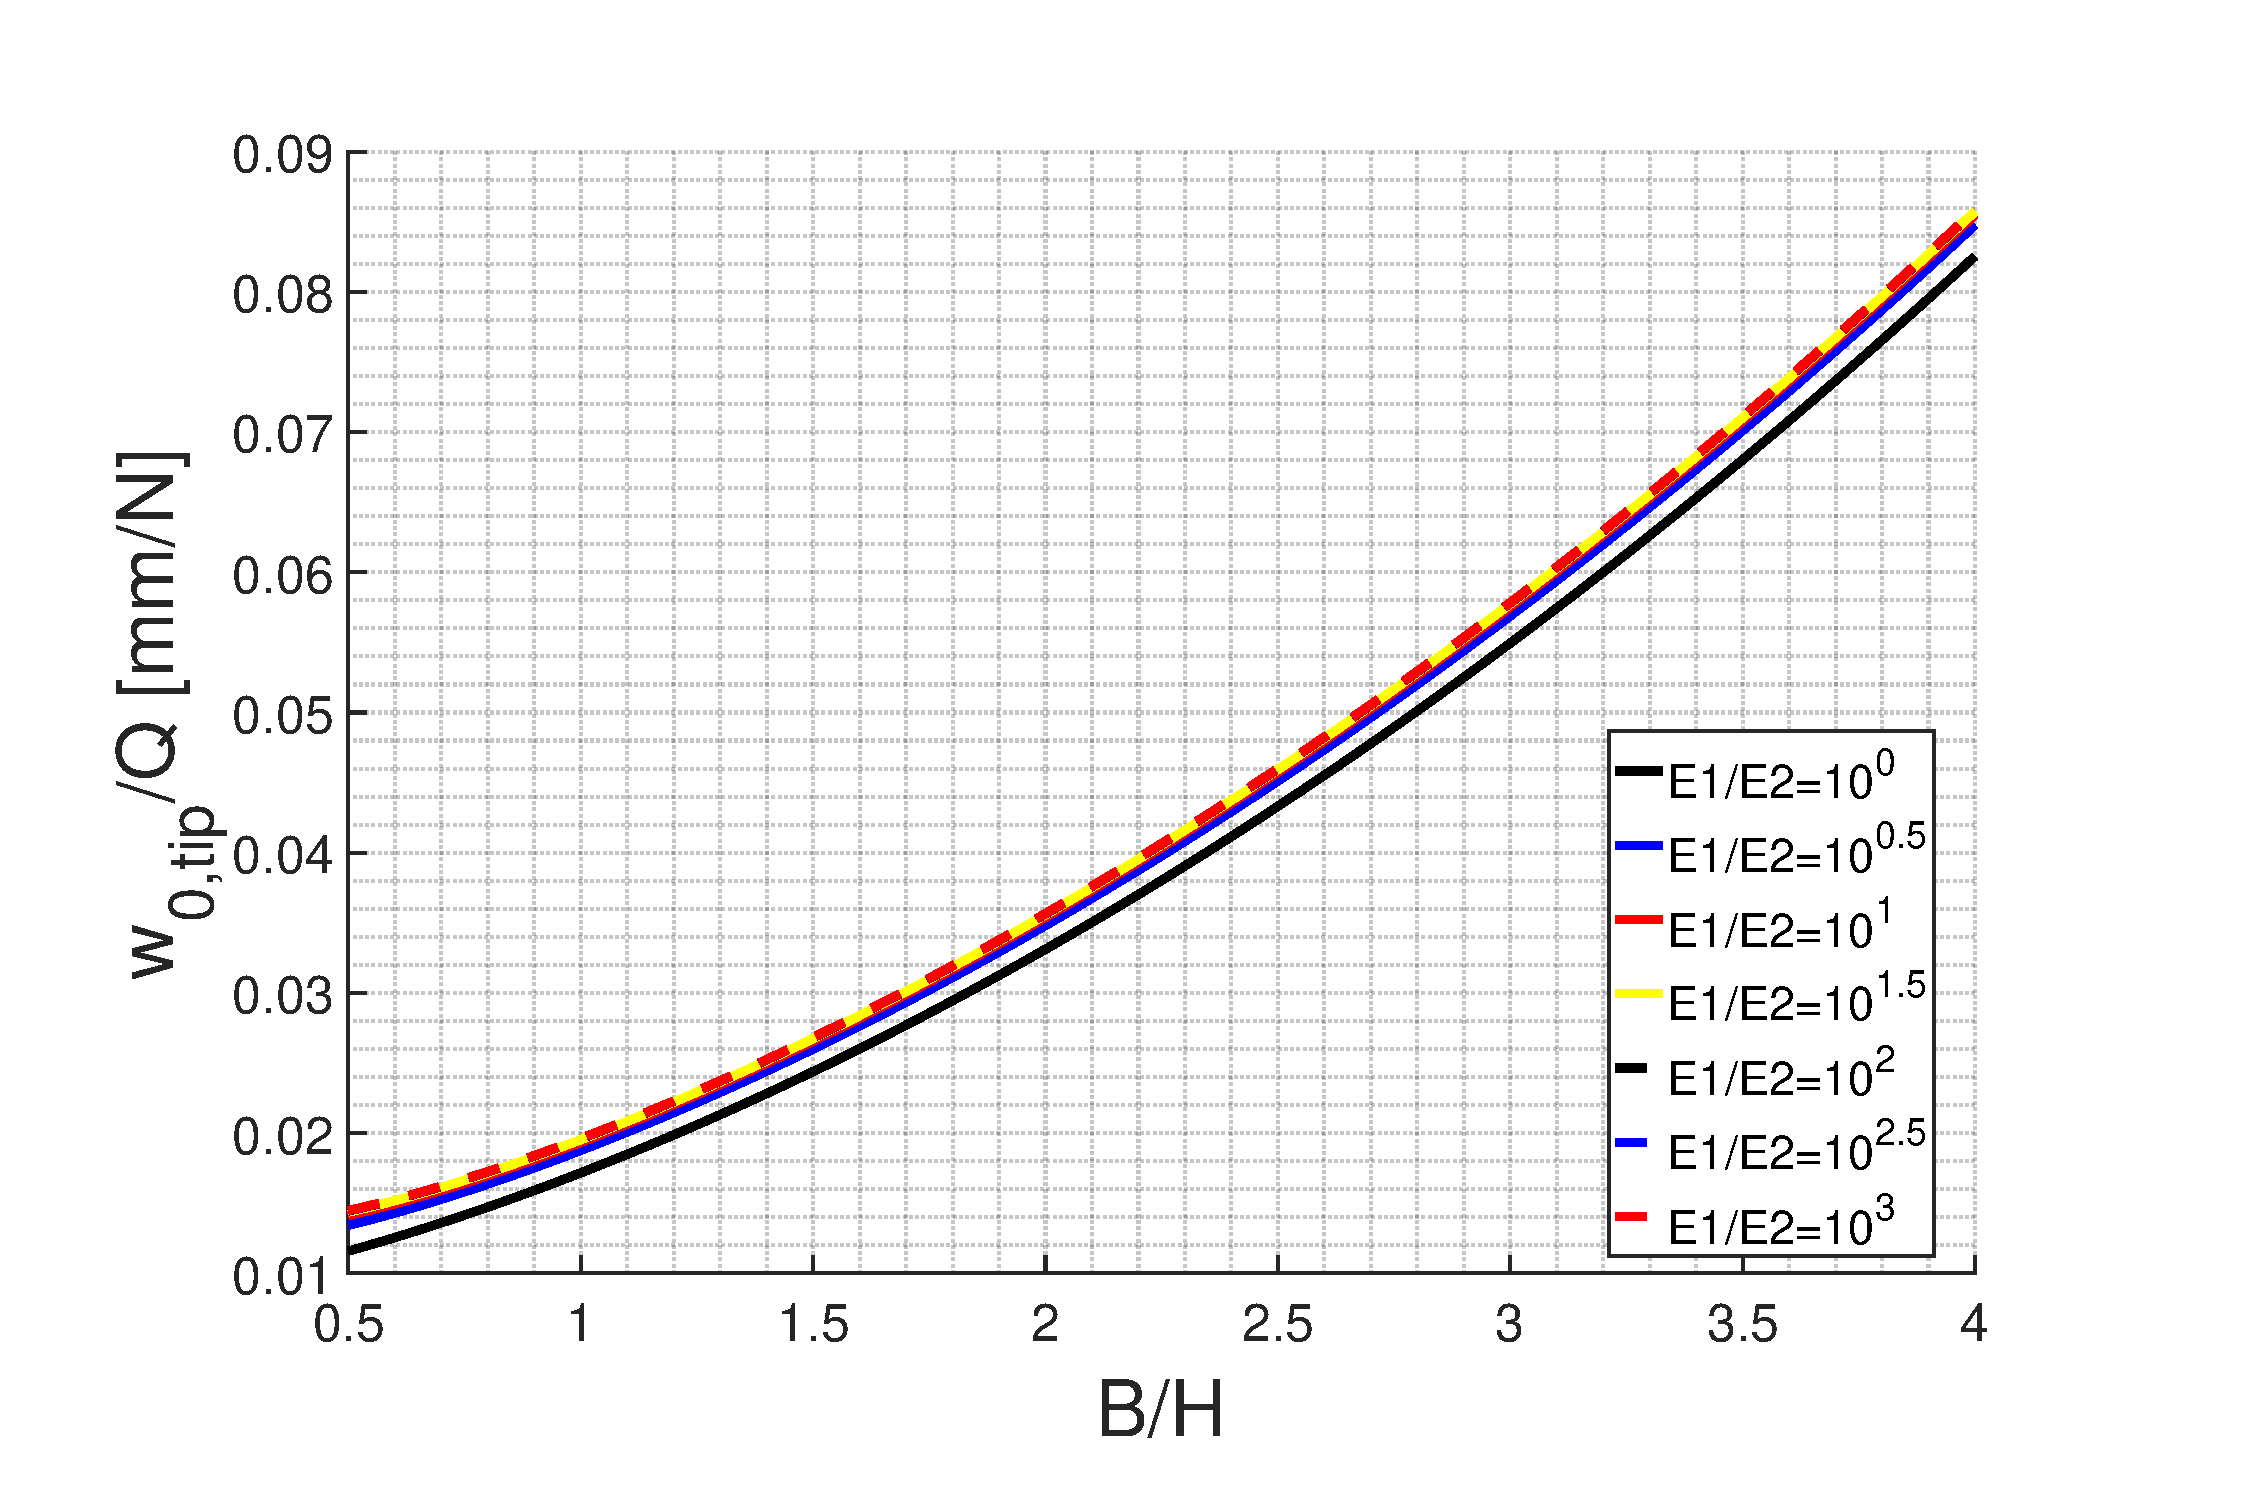
\includegraphics[width=0.8 \textwidth]{../../analytical/figures/woverQ-E1overE2-BoverH}
  \caption[Influence of the cross-sectional aspect ratio $B/H$ on the deflection compliance]{Influence of the cross-sectional aspect ratio $B/H$ on the deflection compliance $w_{\mathrm{0,tip}} / Q$ is shown for various values of the stiffness ratio $E_1/E_2$ ranging from $10^0$ to $10^3$. }\label{fig:woverQ-E1overE2-BoverH}
\end{figure}

\begin{figure}[!htpb] %\phi_tip / Q versus B/H, torsional compliance
  \centering
  \includegraphics[width=0.8 \textwidth]{../../analytical/figures/phioverQ-E1overE2-BoverH}
  \caption[Influence of the cross-sectional aspect ratio $B/H$ on the torsional compliance]{Influence of the cross-sectional aspect ratio $B/H$ on the torsional compliance $|\phi_{\mathrm{tip}}| / Q$ is shown for various values of the stiffness ratio $E_1/E_2$ ranging from $10^0$ to $10^3$. }\label{fig:phioverQ-E1overE2-BoverH}
\end{figure}

%%%% Figures variation of t2/t1
\begin{figure}[!htpb] %G I_t versus t2/t1
  \centering
  \includegraphics[width=0.8 \textwidth]{../../analytical/figures/GIt-E1overE2-t2overt1}
  \caption[Influence of the wall thickness ratio $t_2/t_1$ on the torsional stiffness $GI_t$]{Influence of the wall thickness ratio $t_2/t_1$ on the torsional stiffness $GI_t$ shown for various values of the stiffness ratio $E_1/E_2$ ranging from $10^0$ to $10^3$. }\label{fig:GIt-E1overE2-t2overt1}
\end{figure}

\begin{figure}[!htpb] %Shear centre versus t2/t1
  \centering
  \includegraphics[width=0.8 \textwidth]{../../analytical/figures/SC-E1overE2-t2overt1}
  \caption[Influence of the wall thickness ratio $t_2/t_1$ on the dimensionless shear centre position $y_{\mathrm{SC}}/B$]{Influence of the wall thickness ratio $t_2/t_1$ on the dimensionless shear centre position $y_{\mathrm{SC}}/B$ shown for various values of the stiffness ratio $E_1/E_2$ ranging from $10^0$ to $10^3$. }\label{fig:SC-E1overE2-t2overt1}
\end{figure}

\begin{figure}[!htpb] %E I_y = \Phi_y versus t2/t1
  \centering
  \includegraphics[width=0.8 \textwidth]{../../analytical/figures/EIy-E1overE2-t2overt1}
  \caption[Influence of the wall thickness ratio $t_2/t_1$ on the flexural stiffness $EI_y$]{Influence of the wall thickness ratio $t_2/t_1$ on the flexural stiffness $EI_y = \Phi_y$ shown for various values of the stiffness ratio $E_1/E_2$ ranging from $10^0$ to $10^3$. }\label{fig:EIy-E1overE2-t2overt1}
\end{figure}

\begin{figure}[!htpb] %w_0,tip / Q versus t2/t1, deflection compliance
  \centering
  \includegraphics[width=0.8 \textwidth]{../../analytical/figures/woverQ-E1overE2-t2overt1}
  \caption[Influence of the thickness ratio $t2/t1$ on the deflection compliance]{Influence of the thickness ratio $t2/t1$ on the deflection compliance $w_{\mathrm{0,tip}} / Q$ is shown for various values of the stiffness ratio $E_1/E_2$ ranging from $10^0$ to $10^3$. }\label{fig:woverQ-E1overE2-t2overt1}
\end{figure}

\begin{figure}[!htpb] %\phi_tip / Q versus t2/t1, torsional compliance
  \centering
  \includegraphics[width=0.8 \textwidth]{../../analytical/figures/phioverQ-E1overE2-t2overt1}
  \caption[Influence of the thickness ratio $t2/t1$ on the torsional compliance]{Influence of the thickness ratio $t2/t1$ on the torsional compliance $|\phi_{\mathrm{tip}}| / Q$ is shown for various values of the stiffness ratio $E_1/E_2$ ranging from $10^0$ to $10^3$. }\label{fig:phioverQ-E1overE2-t2overt1}
\end{figure}

%%%% Figures variation of L / B
\begin{figure}[!htpb] %w_0,tip / Q versus L/B, deflection compliance
  \centering
  \includegraphics[width=0.8 \textwidth]{../../analytical/figures/woverQ-E1overE2-LoverB}
  \caption[Influence of the slenderness ratio $L/B$ on the deflection compliance]{Influence of the slenderness ratio $L/B$ on the deflection compliance $w_{\mathrm{0,tip}} / Q$ is shown for various values of the stiffness ratio $E_1/E_2$ ranging from $10^0$ to $10^3$. }\label{fig:woverQ-E1overE2-LoverB}
\end{figure}

\begin{figure}[!htpb] %\phi_tip / Q versus L/B, torsional compliance
  \centering
  \includegraphics[width=0.8 \textwidth]{../../analytical/figures/phioverQ-E1overE2-LoverB}
  \caption[Influence of the slenderness ratio $L/B$ on the torsional compliance]{Influence of the slenderness ratio $L/B$ on the torsional compliance $|\phi_{\mathrm{tip}}| / Q$ is shown for various values of the stiffness ratio $E_1/E_2$ ranging from $10^0$ to $10^3$. }\label{fig:phioverQ-E1overE2-LoverB}
\end{figure}

\clearpage
\subsubsection{Discussion of the results} \label{subsubsec:disc_results_parametricStudy}

The maximum torsional stiffness $G I_t$ as a function on the cross-sectional aspect ratio $B/H$ can be visualized in Figure \ref{fig:GIt-E1overE2-BoverH}. It can be seen that it appears for $B/H = 1$ when $E_1/E_2 = 1$. Therefore, as it is also shown in \cite{Raither2013a}, the closer the torsional stiffness to the doubly symmetric case, the higher its torsional stiffness. However, when $E_1/E_2 > 10$, the maximum torsional stiffness is shown to appear for $B/H > 1$. A similar conclusion can be extract when analysing the Figure \ref{fig:GIt-E1overE2-t2overt1}, that shows the influence of the thickness ratio $t_2/t_1$ on the torsional stiffness $G I_t$.

In Figure \ref{fig:SC-E1overE2-BoverH} it can be seen that for values $E_2 \ll E_1$, the shear centre position $y_{\mathrm{SC}}$ is approximately constant for $B/H$ variations. In this context, the beam approximates its behavior as if it has an open profile section. However, as the value of $E_1/E_2$ decreases, the influence of the ratio $B/H$ increases showing a bigger influence of the web where the Young's modulus $E_2$ applies. On the other hand, Figure \ref{fig:SC-E1overE2-t2overt1} shows that the bigger the thickness ratio $t_2/t_1$ is, the closer that the shear centre $y_{\mathrm{SC}}$ will be to the vertical axis of simmetry. However, for $E_2 \ll E_1$ the influence of the thickness ratio $t_2/t_1$ is reduced.

The influence of the cross-sectional aspect ratio $B/H$ and the tickness ratio $t_2/t_1$ on the flexural stiffness $E I_y$ is shown to be bigger that that of the Young's modulus ratio $E_1/E_2$, as shown on Figures \ref{fig:EIy-E1overE2-BoverH} and \ref{fig:EIy-E1overE2-t2overt1}, respectively.

% The beam torsional compliance is highly dependant on that torsional moment applied on the beam, that depends on the shear centre $y_{\mathrm{SC}} position. Therefore, as shown on Figure \ref{fig:phioverQ-E1overE2-t2overt1}, the beam's torsional compliance is approximately constant for values of thickness ratio $t_2/t_1 > 1$.


%Comparison of the torsional compliance at the tip against stiffness ratio
\chapter{Conclusion and Outlook} \label{chap:summary}
%
%Outlook:
% - To improve the mesh characteristics (to avoid distorted elements)
%
%Summary:

This thesis presents a novel passive mechanism for achieving wing twist morphing by means of modifying the bending-twist coupling of wing structures. The system incorporates a variable-stiffness spar in the wing-box that comprises a lattice of chiral elements. In the ligaments of these elements, elastic instabilities are intentionally induced and thus the effective shear modulus of the adaptive spar is modified. This phenomena provokes the wing-box section shear centre shifting and the consequent modification in wing-box torsional stiffness. This induces a wing-box twist adaptation that has been passively activated exploiting local elastic instabilities.

An analytical model of the wing-box is developed using an ideal beam configuration with variable shear modulus in one of the webs. The effect of variations of this magnitude on the torsional stiffness, the flexural stiffness, the shear centre position and the bending and twisting deformations of the wing-box are studied. Also, the effect of variations of the geometry in these magnitudes is analysed. Results show that, once the buckling-induced reduction in shear modulus in the spar is activated, the reduction in flexural stiffness for the wing-box is negligible compared with the reduction in torsional stiffness. 

A computational model of the simplified wing-box is built next. It is designed in a fully parameterized format using Python scripting. This model is constituted of a wing-box in C-profile, a lattice of chiral elements and a number of ribs that provide additional transversal stiffness and avoid local deformations in the wing-box skin. Different design options are considered, such as variations in the geometry, the load, the mesh and the number of ribs. An analysis of this model is performed in order to obtain a baseline configuration to posteriorly execute parametric studies. One of the aspects considered is the modeling of the lattice nodes rigid body behavior. Results shows that the most suitable modeling approach is to add an additional rigid part to provide supplementary stiffness. The addition of ribs in the middle of wing-box length is necessary to provide additional stiffness in the transversal direction and prevent undesired local deformations in the wing-box skin. Another consideration is the appearance of sources of instabilities such as buckling that require the inclusion of artificial damping factor into the simulation. 

Nonlinear simulations are carried out using this model and incorporating artificial energy dissipation through constant damping factor. The onset of the buckling phenomena and its evolution in the chiral lattice is characterized next. Results show that the collapse of the structure occurs when severe buckling appears on the ligaments of the chiral elements located at the root of the wing-box. This event produces a sudden reduction on the torsional stiffness of the structure and an increase in the wing-box twist adaptation observed at the tip. A second and more generalized buckling in the chiral lattice is observed to origin a second modification of the torsional stiffness for certain cases. In the baseline configuration, the length of the wing-box is 0.743 m, the width is 0.3 m and the height is 0.383 m. The load condition is a single point load applied on the upper flange of the tip rib and in the middle point of the width. For this case, the twist morphing of the wing-box is obtained to be equal to -1.25 degrees for the nonlinear simulation while the predicted twist for the linear simulation is -0.19 degrees.

Furthermore, a parametric study is performed on the computational model of the wing-box. Results show that considerable tailorability can be achieved through modifications of selected parameters. The parameter that displays a bigger influence in the onset and evolution of the elastic instabilities is the wing-box thickness. Increasing the wing-box thickness by 0.1 mm, provokes that the required force to induce the appearance of buckling at the root increases by 100 N. 

A wing model featuring a compliant spar design with the lattice of chiral elements is introduced to test the feasibility of the proposed concept under realistic aerodynamic loads. A weakly coupled aeroelastic analysis is performed with this model. The particular simulation case considers a wing with span equal 3 m, chord length equal to 0.5 m and air velocity of 30 m/s. The achieved twist deformation for this case was of about 4 degrees at the wing tip. Results from the simulations show that the wing twist adaptation increases as the air velocity increases. A single case was considered and, for it, the nonlinear and linear simulations displayed similar results. The developed model is fully parameterized and enables multiple parameter variations that would make it possible to achieve a more suitable wing configuration.  

In further studies of this technology, it would be necessary to numerically analyse the wing root bending moment variation after the mechanism activation and also manufacture a demonstrator that could be used to experimentally test the feasibility of the proposed concept. The analysis of the time-bounded response of this mechanism is beyond the scope of this preliminary work, but such a investigation would be a crucial prior implementation of the system on a real lift generating structure.

The proposed morphing has been shown to be capable of inducing global twist morphing of a wing-box exploiting local elastic instabilities. It has shown to be promising to be applied on realistic wing structures for which the torsional response is dominated by the wing-box. Potential applications may include load alleviation purposes on lift-generating structures with high aspect ratio. 

% Bibliography
\newpage
\bibliographystyle{ieeetr}
\bibliography{projectBib}
\addtocontents{toc}{\vspace{.5\baselineskip}}
\addcontentsline{toc}{chapter}{\protect\numberline{}{Bibliography}}
% \renewcommand\refname{Bibliography}


%Appendix if necessary
\newpage
\addtocontents{toc}{\vspace{.5\baselineskip}}
\appendix
\section*{Python code generated} \label{appen:code}

All the code code generated for this project can be downloaded from the following Github repository: \texttt{https://github.com/AlejandroValverde/abaqus.git}.


\end{document}

